%!TEX root = ./RfCPN.tex


\addtocontents{toc}{\protect\cleardoublepage}
%%%%%%%%%%%%%%%%%%%%%%%%%%%%%%%%%%%%%%%%%%%%%%%%%%%%%%%%%
%% Part Requirement Definition %%%%%%%%%%%%%%%%%%%%%%%%%%
%%%%%%%%%%%%%%%%%%%%%%%%%%%%%%%%%%%%%%%%%%%%%%%%%%%%%%%%%
\addtocontents{toc}{\protect\begin{tocBox}{\tmppartnum}}%
\tPart[lof]{加工システムの設計\TBW}{%
\paragraph*{\tpartgoal}
加工システムの作成に向けて、その設計を行う。

\tcbline*
\paragraph*{\tpartmethod}
策定した諸標準や解析的・数値的導出した幾何的情報を用いて、抽出した\index{ようけん@要件}要件を満たすよう設計を行う。

\tcbline*
\paragraph*{\tpartbackground}
(to be written...)
}{%
\paragraph*{\tpartconclusion}
(to be written...)
\tcbline*
\paragraph*{\tpartnextstep}
設計にしたがって、具体的な\index{NCプログラム}NCプログラムの作成を行う。
}

%%%%%%%%%%%%%%%%%%%%%%%%%%%%%%%%%%%%%%%%%%%%%%%%%%%%%%%%%
%% chapters %%%%%%%%%%%%%%%%%%%%%%%%%%%%%%%%%%%%%%%%%%%%%
%%%%%%%%%%%%%%%%%%%%%%%%%%%%%%%%%%%%%%%%%%%%%%%%%%%%%%%%%
%!TEX root = ../RfCPN.tex


\modHeadchapter[lof]{加工システムの全体の流れ}



%%%%%%%%%%%%%%%%%%%%%%%%%%%%%%%%%%%%%%%%%%%%%%%%%%%%%%%%%%
%% section 06.01 %%%%%%%%%%%%%%%%%%%%%%%%%%%%%%%%%%%%%%%%%
%%%%%%%%%%%%%%%%%%%%%%%%%%%%%%%%%%%%%%%%%%%%%%%%%%%%%%%%%%
\modHeadsection{加工全体の流れ}
加工全体の流れは\pageautoref{sec:MillingSystemFlow}に基づく。


%%%%%%%%%%%%%%%%%%%%%%%%%%%%%%%%%%%%%%%%%%%%%%%%%%%%%%%%%%
%% subsection 06.02.01 %%%%%%%%%%%%%%%%%%%%%%%%%%%%%%%%%%%
%%%%%%%%%%%%%%%%%%%%%%%%%%%%%%%%%%%%%%%%%%%%%%%%%%%%%%%%%%
\subsection{工程:加工前の段取}
\begin{enumerate}[label*=\sarrow]
\item ワークを\Table 上の\Jig に取り付ける
\item \Palette を交換し、ワークを機内に搬入する
\end{enumerate}


%%%%%%%%%%%%%%%%%%%%%%%%%%%%%%%%%%%%%%%%%%%%%%%%%%%%%%%%%%
%% subsection 06.02.02 %%%%%%%%%%%%%%%%%%%%%%%%%%%%%%%%%%%
%%%%%%%%%%%%%%%%%%%%%%%%%%%%%%%%%%%%%%%%%%%%%%%%%%%%%%%%%%
\subsection{工程:加工前の測定}

%%%%%%%%%%%%%%%%%%%%%%%%%%%%%%%%%%%%%%%%%%%%%%%%%%%%%%%%%%
%% subsubsection 06.02.02.1 %%%%%%%%%%%%%%%%%%%%%%%%%%%%%%
%%%%%%%%%%%%%%%%%%%%%%%%%%%%%%%%%%%%%%%%%%%%%%%%%%%%%%%%%%
\subsubsection{ワーク座標系原点設定}
\begin{enumerate}[label*=\sarrow]
\item ボトム側が工具側になるよう回転する
\item \BottomEndFace 部の外側中心を測定する
\item \BottomEndFace 部の内側中心を測定する
\item トップ側が工具側になるよう回転する
\item \TopEndFace 部の外側中心を測定する
\item \TopEndFace 部の内側中心を測定する
\item \KeywayCenter を測定する
\end{enumerate}

%%%%%%%%%%%%%%%%%%%%%%%%%%%%%%%%%%%%%%%%%%%%%%%%%%%%%%%%%%
%% subsubsection 06.02.02.1 %%%%%%%%%%%%%%%%%%%%%%%%%%%%%%
%%%%%%%%%%%%%%%%%%%%%%%%%%%%%%%%%%%%%%%%%%%%%%%%%%%%%%%%%%
\subsubsection{\DimpleMeasurement}
\begin{enumerate}[label*=\sarrow]
\item すべての\Dimple の表面位置を測定する
\end{enumerate}


%%%%%%%%%%%%%%%%%%%%%%%%%%%%%%%%%%%%%%%%%%%%%%%%%%%%%%%%%%
%% subsection 06.02.03 %%%%%%%%%%%%%%%%%%%%%%%%%%%%%%%%%%%
%%%%%%%%%%%%%%%%%%%%%%%%%%%%%%%%%%%%%%%%%%%%%%%%%%%%%%%%%%
\subsection{工程:トップ側の加工}
\begin{enumerate}[label*=\sarrow]
\item \DimpleMilling を行う
\item \TopEndFacecutMilling を行う
\item (存在する場合)\TopOutcutMilling を行う
\item (存在する場合)\TopCurvedOutcutMilling を行う
\item (存在する場合)\EndFaceBoringMilling を行う
\item (存在する場合)\IncutBoringMilling を行う
\item \TopEndFaceOutCChamferMilling を行う
\item \TopEndFaceInCChamferMilling を行う
\end{enumerate}


\clearpage
%%%%%%%%%%%%%%%%%%%%%%%%%%%%%%%%%%%%%%%%%%%%%%%%%%%%%%%%%%
%% subsection 06.02.04 %%%%%%%%%%%%%%%%%%%%%%%%%%%%%%%%%%%
%%%%%%%%%%%%%%%%%%%%%%%%%%%%%%%%%%%%%%%%%%%%%%%%%%%%%%%%%%
\subsection{工程:ボトム側の加工}
\begin{enumerate}[label*=\sarrow]
\item ボトム側が工具側になるよう回転する
\item \BottomEndFacecutMilling を行う
\item (存在する場合)\BottomOutcutMilling を行う
\item (存在する場合)\BottomCurvedOutcutMilling を行う
\item \BottomEndFaceOutCChamferMilling を行う
\item \BottomEndFaceInCChamferMilling を行う
\end{enumerate}


%%%%%%%%%%%%%%%%%%%%%%%%%%%%%%%%%%%%%%%%%%%%%%%%%%%%%%%%%%
%% subsection 06.02.05 %%%%%%%%%%%%%%%%%%%%%%%%%%%%%%%%%%%
%%%%%%%%%%%%%%%%%%%%%%%%%%%%%%%%%%%%%%%%%%%%%%%%%%%%%%%%%%
\subsection{工程:加工後の測定}
\begin{enumerate}[label*=\sarrow]
\item \TopOutcut と\BottomOutcut の両方が存在する場合、\CenterlineEndFaceDifMeasurement を行う
\end{enumerate}


%%%%%%%%%%%%%%%%%%%%%%%%%%%%%%%%%%%%%%%%%%%%%%%%%%%%%%%%%%
%% subsection 41.01.06 %%%%%%%%%%%%%%%%%%%%%%%%%%%%%%%%%%%
%%%%%%%%%%%%%%%%%%%%%%%%%%%%%%%%%%%%%%%%%%%%%%%%%%%%%%%%%%
\subsection{工程:加工後の段取}
\begin{enumerate}[label*=\sarrow]
\item \Palette を交換し、ワークを機外に搬出する
\item ワークを\Table 上の\Jig から取り外す
\end{enumerate}


%%%%%%%%%%%%%%%%%%%%%%%%%%%%%%%%%%%%%%%%%%%%%%%%%%%%%%%%%%
%% figure %%%%%%%%%%%%%%%%%%%%%%%%%%%%%%%%%%%%%%%%%%%%%%%%
%%%%%%%%%%%%%%%%%%%%%%%%%%%%%%%%%%%%%%%%%%%%%%%%%%%%%%%%%%
\begin{figure}[p]%
\begin{Figlandscape}
\begin{adjustbox}{%
  addcode={\begin{minipage}{\textheight}\centering}{%
    \captionof{figure}{加工全体のフロー(概要):加工前段取~測定\label{fig:flowchartFirst}}%
    \end{minipage}%
  },
  rotate=90,
  center,
%  max width=\textheight,
%  max height=\linewidth,
  keepaspectratio}
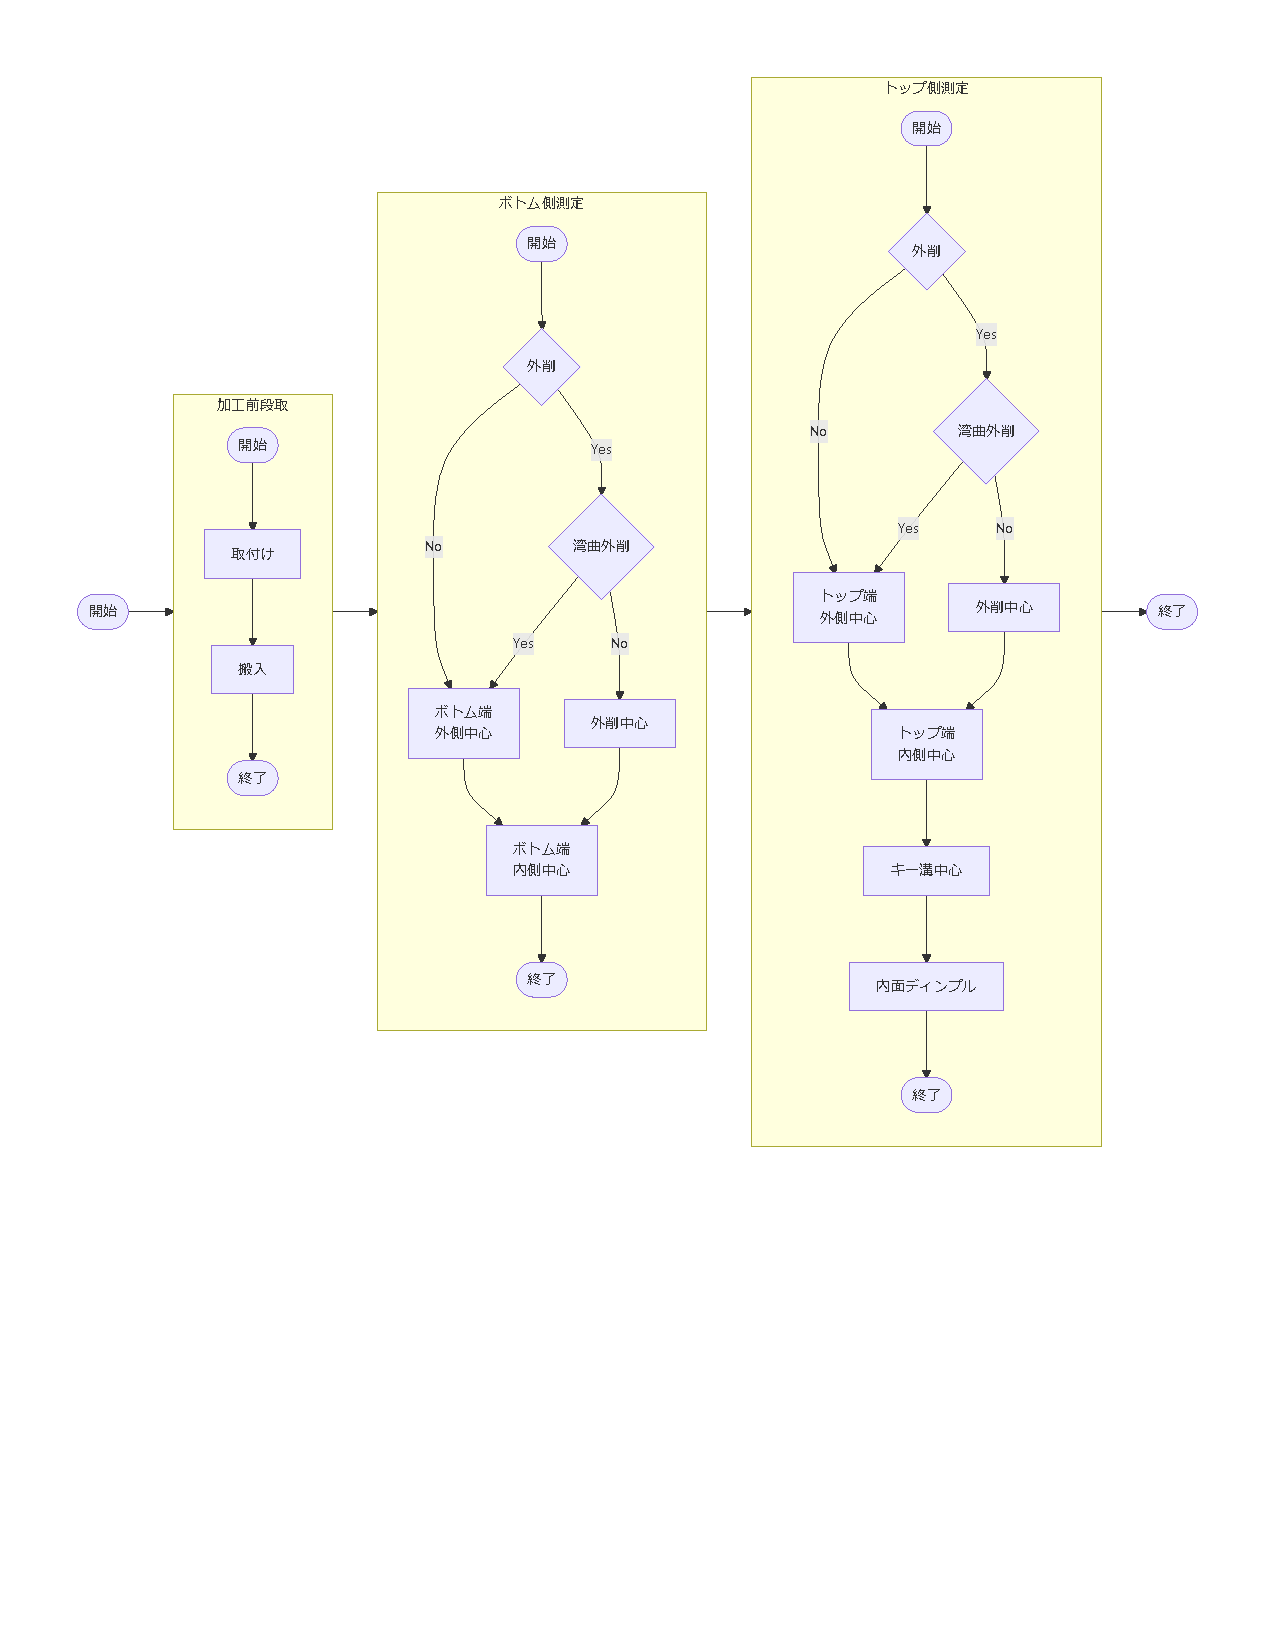
\includegraphics[height=\linewidth-10pt, trim=0 235 0 20, clip]{RfCPN_p03_pictures/Measurement_flow_chart.pdf}%
\end{adjustbox}
\end{Figlandscape}%
\end{figure}%
%%%%%%%%%%%%%%%%%%%%%%%%%%%%%%%%%%%%%%%%%%%%%%%%%%%%%%%%%%
%%%%%%%%%%%%%%%%%%%%%%%%%%%%%%%%%%%%%%%%%%%%%%%%%%%%%%%%%%
%%%%%%%%%%%%%%%%%%%%%%%%%%%%%%%%%%%%%%%%%%%%%%%%%%%%%%%%%%


%%%%%%%%%%%%%%%%%%%%%%%%%%%%%%%%%%%%%%%%%%%%%%%%%%%%%%%%%%
%% figure %%%%%%%%%%%%%%%%%%%%%%%%%%%%%%%%%%%%%%%%%%%%%%%%
%%%%%%%%%%%%%%%%%%%%%%%%%%%%%%%%%%%%%%%%%%%%%%%%%%%%%%%%%%
\begin{figure}[p]%
\begin{Figlandscape}
\begin{adjustbox}{%
  addcode={\begin{minipage}{\textheight}\centering}{%
    \captionof{figure}{加工全体のフロー(概要):加工~加工後段取\label{fig:flowchartSecond}}%
    \end{minipage}%
  },
  rotate=90,
  center,
%  max width=\textheight,
%  max height=\linewidth,
  keepaspectratio}
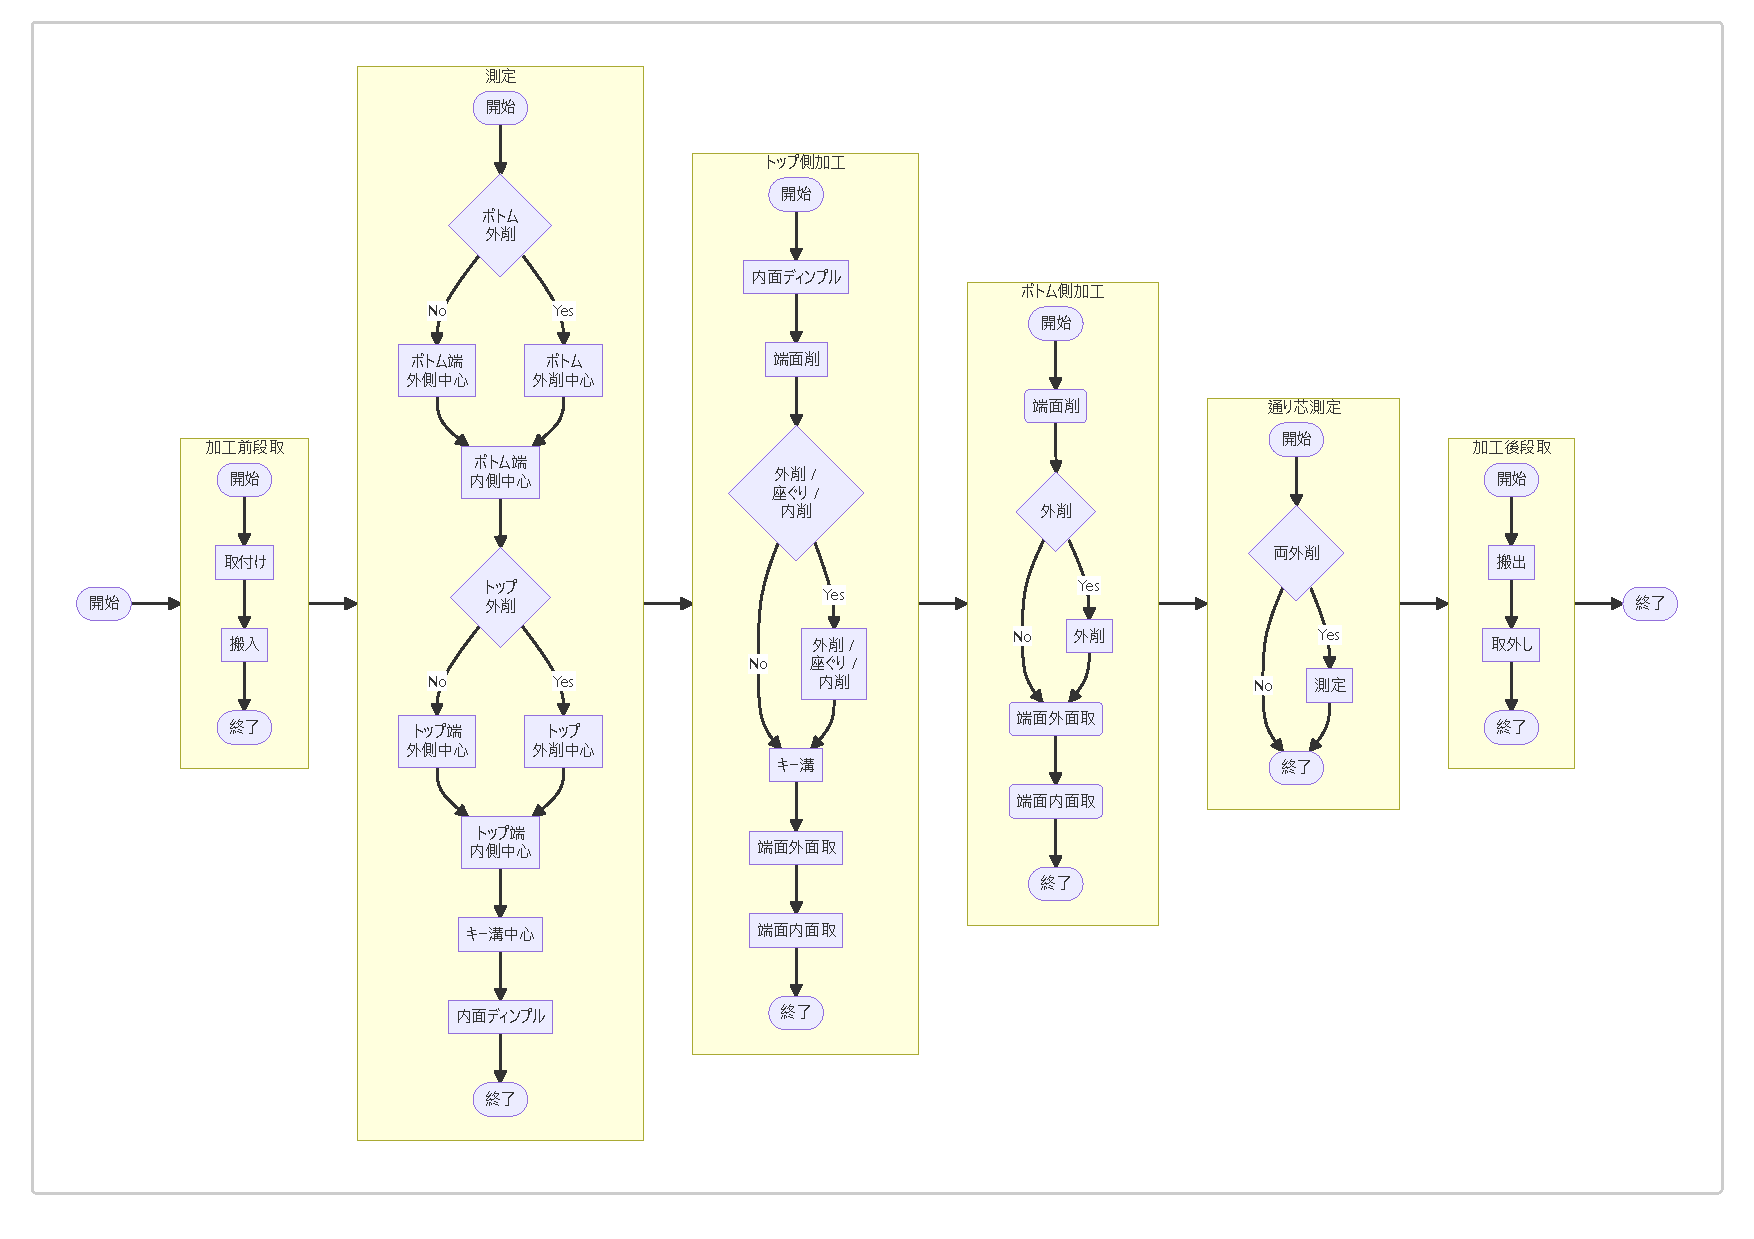
\includegraphics[height=\linewidth-10pt, trim=0 205 0 20, clip]{RfCPN_p03_pictures/Milling_flow_chart.pdf}%
\end{adjustbox}
\end{Figlandscape}%
\end{figure}%
%%%%%%%%%%%%%%%%%%%%%%%%%%%%%%%%%%%%%%%%%%%%%%%%%%%%%%%%%%
%%%%%%%%%%%%%%%%%%%%%%%%%%%%%%%%%%%%%%%%%%%%%%%%%%%%%%%%%%
%%%%%%%%%%%%%%%%%%%%%%%%%%%%%%%%%%%%%%%%%%%%%%%%%%%%%%%%%%



%!TEX root = ../RfCPN.tex


\modHeadchapter{ワーク座標系原点および加工基準点}
\DMC では、\index{ワークざひょうけいげんてん@ワーク座標系原点}ワーク座標系を明細に依存しないよう設定を行うものとする。
また、どのワーク座標系の原点を基準として各工程の加工を行うかを定める。


%%%%%%%%%%%%%%%%%%%%%%%%%%%%%%%%%%%%%%%%%%%%%%%%%%%%%%%%%%
%% section 38.01 %%%%%%%%%%%%%%%%%%%%%%%%%%%%%%%%%%%%%%%%%
%%%%%%%%%%%%%%%%%%%%%%%%%%%%%%%%%%%%%%%%%%%%%%%%%%%%%%%%%%
\modHeadsection{ワーク座標系の種類}
\DMC で用いられているワーク座標系には以下のものがある。
\begin{enumerate}[label*=\sarrow]
\item {\ttfamily G53}
\item {\ttfamily G54} - {\ttfamily G59}
\item {\ttfamily G54.1\;P01} - {\ttfamily G54.1\;P96}
\end{enumerate}
ただし、{\ttfamily G53}は\index{きかいざひょうけい@機械座標系}機械座標系である。



%%%%%%%%%%%%%%%%%%%%%%%%%%%%%%%%%%%%%%%%%%%%%%%%%%%%%%%%%%
%% section 38.02 %%%%%%%%%%%%%%%%%%%%%%%%%%%%%%%%%%%%%%%%%
%%%%%%%%%%%%%%%%%%%%%%%%%%%%%%%%%%%%%%%%%%%%%%%%%%%%%%%%%%
\modHeadsection{ワーク座標系{\ttfamily G54}}
ワーク座標系{\ttfamily G54}は、主にボトム側の外側中心を示すものとする。


%%%%%%%%%%%%%%%%%%%%%%%%%%%%%%%%%%%%%%%%%%%%%%%%%%%%%%%%%%
%% subsection 38.02.01 %%%%%%%%%%%%%%%%%%%%%%%%%%%%%%%%%%%
%%%%%%%%%%%%%%%%%%%%%%%%%%%%%%%%%%%%%%%%%%%%%%%%%%%%%%%%%%
\subsection{ワーク座標系{\ttfamily G54X}の原点}
\begin{enumerate}[label*=\sarrow]
\item \BottomOutcut(\BottomCurvedOutcut を除く)がない場合は、\BottomEndFace 部AC方向外側中心の測定値
\item \BottomOutcut(\BottomCurvedOutcut を除く)があり、かつ\OutcutCenter の基準が\BottomOutcut にある場合、ボトム側のAC方向\OutcutCenter の測定値
\item \BottomOutcut(\BottomCurvedOutcut を除く)があり、かつ\OutcutCenter の基準が\TopOutcut にある場合、{\ttfamily G56X}から\CenterlineEndFaceDif 寸法を加味した計算値
\end{enumerate}


%%%%%%%%%%%%%%%%%%%%%%%%%%%%%%%%%%%%%%%%%%%%%%%%%%%%%%%%%%
%% subsection 38.02.02 %%%%%%%%%%%%%%%%%%%%%%%%%%%%%%%%%%%
%%%%%%%%%%%%%%%%%%%%%%%%%%%%%%%%%%%%%%%%%%%%%%%%%%%%%%%%%%
\subsection{ワーク座標系{\ttfamily G54Y}の原点}
\begin{enumerate}[label*=\sarrow]
\item \BottomOutcut(\BottomCurvedOutcut を含む)がない場合は、\BottomEndFace 部BD方向外側中心の測定値
\item \BottomOutcut(\BottomCurvedOutcut を含む)がある場合は、{\ttfamily G55Y}の値
\end{enumerate}


%%%%%%%%%%%%%%%%%%%%%%%%%%%%%%%%%%%%%%%%%%%%%%%%%%%%%%%%%%
%% subsection 38.02.03 %%%%%%%%%%%%%%%%%%%%%%%%%%%%%%%%%%%
%%%%%%%%%%%%%%%%%%%%%%%%%%%%%%%%%%%%%%%%%%%%%%%%%%%%%%%%%%
\subsection{ワーク座標系{\ttfamily G54Z}の原点\TBW}


%%%%%%%%%%%%%%%%%%%%%%%%%%%%%%%%%%%%%%%%%%%%%%%%%%%%%%%%%%
%% subsection 38.02.04 %%%%%%%%%%%%%%%%%%%%%%%%%%%%%%%%%%%
%%%%%%%%%%%%%%%%%%%%%%%%%%%%%%%%%%%%%%%%%%%%%%%%%%%%%%%%%%
\subsection{ワーク座標系{\ttfamily G54B}の原点}
\Jig の工具側面が$XY$平面と平行となる角度において絶対値が最小のもの


%%%%%%%%%%%%%%%%%%%%%%%%%%%%%%%%%%%%%%%%%%%%%%%%%%%%%%%%%%
%% subsection 38.02.05 %%%%%%%%%%%%%%%%%%%%%%%%%%%%%%%%%%%
%%%%%%%%%%%%%%%%%%%%%%%%%%%%%%%%%%%%%%%%%%%%%%%%%%%%%%%%%%
\subsection{ワーク座標系{\ttfamily G54C}の原点}
ワーク座標系{\ttfamily G54C}は、使用しない。



\clearpage
%%%%%%%%%%%%%%%%%%%%%%%%%%%%%%%%%%%%%%%%%%%%%%%%%%%%%%%%%%
%% section 38.03 %%%%%%%%%%%%%%%%%%%%%%%%%%%%%%%%%%%%%%%%%
%%%%%%%%%%%%%%%%%%%%%%%%%%%%%%%%%%%%%%%%%%%%%%%%%%%%%%%%%%
\modHeadsection{ワーク座標系{\ttfamily G55}}
ワーク座標系{\ttfamily G55}は、主にボトム側の内側中心を示すものとする。


%%%%%%%%%%%%%%%%%%%%%%%%%%%%%%%%%%%%%%%%%%%%%%%%%%%%%%%%%%
%% subsection 38.03.01 %%%%%%%%%%%%%%%%%%%%%%%%%%%%%%%%%%%
%%%%%%%%%%%%%%%%%%%%%%%%%%%%%%%%%%%%%%%%%%%%%%%%%%%%%%%%%%
\subsection{ワーク座標系{\ttfamily G55X}の原点}
\begin{enumerate}[label*=\sarrow]
\item \BottomEndFace 部AC方向内側中心の測定値
\end{enumerate}


%%%%%%%%%%%%%%%%%%%%%%%%%%%%%%%%%%%%%%%%%%%%%%%%%%%%%%%%%%
%% subsection 38.03.02 %%%%%%%%%%%%%%%%%%%%%%%%%%%%%%%%%%%
%%%%%%%%%%%%%%%%%%%%%%%%%%%%%%%%%%%%%%%%%%%%%%%%%%%%%%%%%%
\subsection{ワーク座標系{\ttfamily G55Y}の原点}
\begin{enumerate}[label*=\sarrow]
\item \BottomEndFace 部BD方向内側中心の測定値
\end{enumerate}


%%%%%%%%%%%%%%%%%%%%%%%%%%%%%%%%%%%%%%%%%%%%%%%%%%%%%%%%%%
%% subsection 38.03.03 %%%%%%%%%%%%%%%%%%%%%%%%%%%%%%%%%%%
%%%%%%%%%%%%%%%%%%%%%%%%%%%%%%%%%%%%%%%%%%%%%%%%%%%%%%%%%%
\subsection{ワーク座標系{\ttfamily G55Z}の原点\TBW}


%%%%%%%%%%%%%%%%%%%%%%%%%%%%%%%%%%%%%%%%%%%%%%%%%%%%%%%%%%
%% subsection 38.03.04 %%%%%%%%%%%%%%%%%%%%%%%%%%%%%%%%%%%
%%%%%%%%%%%%%%%%%%%%%%%%%%%%%%%%%%%%%%%%%%%%%%%%%%%%%%%%%%
\subsection{ワーク座標系{\ttfamily G55B}の原点}
\Jig の工具側面が$XY$平面と平行となる角度において絶対値が最小のもの


%%%%%%%%%%%%%%%%%%%%%%%%%%%%%%%%%%%%%%%%%%%%%%%%%%%%%%%%%%
%% subsection 38.03.05 %%%%%%%%%%%%%%%%%%%%%%%%%%%%%%%%%%%
%%%%%%%%%%%%%%%%%%%%%%%%%%%%%%%%%%%%%%%%%%%%%%%%%%%%%%%%%%
\subsection{ワーク座標系{\ttfamily G55C}の原点}
ワーク座標系{\ttfamily G55C}は、使用しない。



\clearpage
%%%%%%%%%%%%%%%%%%%%%%%%%%%%%%%%%%%%%%%%%%%%%%%%%%%%%%%%%%
%% section 34.04 %%%%%%%%%%%%%%%%%%%%%%%%%%%%%%%%%%%%%%%%%
%%%%%%%%%%%%%%%%%%%%%%%%%%%%%%%%%%%%%%%%%%%%%%%%%%%%%%%%%%
\modHeadsection{ワーク座標系{\ttfamily G56}}
ワーク座標系{\ttfamily G56}は、主にトップ側の外側中心を示すものとする。


%%%%%%%%%%%%%%%%%%%%%%%%%%%%%%%%%%%%%%%%%%%%%%%%%%%%%%%%%%
%% subsection 34.04.01 %%%%%%%%%%%%%%%%%%%%%%%%%%%%%%%%%%%
%%%%%%%%%%%%%%%%%%%%%%%%%%%%%%%%%%%%%%%%%%%%%%%%%%%%%%%%%%
\subsection{ワーク座標系{\ttfamily G56X}の原点}
\begin{enumerate}[label*=\sarrow]
\item \TopOutcut(\TopCurvedOutcut を除く)がない場合は、\TopEndFace 部AC方向外側中心の測定値
\item \TopOutcut(\TopCurvedOutcut を除く)があり、かつ\OutcutCenter の基準が\TopOutcut にある場合、トップ側のAC方向\OutcutCenter の測定値
\item \TopOutcut(\TopCurvedOutcut を除く)があり、かつ\OutcutCenter の基準が\BottomOutcut にある場合、{\ttfamily G54X}から\CenterlineEndFaceDif 寸法を加味した計算値
\end{enumerate}


%%%%%%%%%%%%%%%%%%%%%%%%%%%%%%%%%%%%%%%%%%%%%%%%%%%%%%%%%%
%% subsection 38.04.02 %%%%%%%%%%%%%%%%%%%%%%%%%%%%%%%%%%%
%%%%%%%%%%%%%%%%%%%%%%%%%%%%%%%%%%%%%%%%%%%%%%%%%%%%%%%%%%
\subsection{ワーク座標系{\ttfamily G56Y}の原点}
\begin{enumerate}[label*=\sarrow]
\item \TopOutcut(\TopCurvedOutcut を含む)がない場合は、\TopEndFace 部BD方向外側中心の測定値
\item \TopOutcut(\TopCurvedOutcut を含む)がある場合は、{\ttfamily G57Y}の値
\end{enumerate}


%%%%%%%%%%%%%%%%%%%%%%%%%%%%%%%%%%%%%%%%%%%%%%%%%%%%%%%%%%
%% subsection 38.04.03 %%%%%%%%%%%%%%%%%%%%%%%%%%%%%%%%%%%
%%%%%%%%%%%%%%%%%%%%%%%%%%%%%%%%%%%%%%%%%%%%%%%%%%%%%%%%%%
\subsection{ワーク座標系{\ttfamily G56Z}の原点\TBW}


%%%%%%%%%%%%%%%%%%%%%%%%%%%%%%%%%%%%%%%%%%%%%%%%%%%%%%%%%%
%% subsection 38.04.04 %%%%%%%%%%%%%%%%%%%%%%%%%%%%%%%%%%%
%%%%%%%%%%%%%%%%%%%%%%%%%%%%%%%%%%%%%%%%%%%%%%%%%%%%%%%%%%
\subsection{ワーク座標系{\ttfamily G56B}の原点}
\Jig の工具側面が$XY$平面と平行となる角度において絶対値が最小のもの


%%%%%%%%%%%%%%%%%%%%%%%%%%%%%%%%%%%%%%%%%%%%%%%%%%%%%%%%%%
%% subsection 38.04.05 %%%%%%%%%%%%%%%%%%%%%%%%%%%%%%%%%%%
%%%%%%%%%%%%%%%%%%%%%%%%%%%%%%%%%%%%%%%%%%%%%%%%%%%%%%%%%%
\subsection{ワーク座標系{\ttfamily G56C}の原点}
ワーク座標系{\ttfamily G56C}は、使用しない。



\clearpage
%%%%%%%%%%%%%%%%%%%%%%%%%%%%%%%%%%%%%%%%%%%%%%%%%%%%%%%%%%
%% section 38.05 %%%%%%%%%%%%%%%%%%%%%%%%%%%%%%%%%%%%%%%%%
%%%%%%%%%%%%%%%%%%%%%%%%%%%%%%%%%%%%%%%%%%%%%%%%%%%%%%%%%%
\modHeadsection{ワーク座標系{\ttfamily G57}}
ワーク座標系{\ttfamily G57}は、主にトップ側の内側中心を示すものとする。


%%%%%%%%%%%%%%%%%%%%%%%%%%%%%%%%%%%%%%%%%%%%%%%%%%%%%%%%%%
%% subsection 38.05.01 %%%%%%%%%%%%%%%%%%%%%%%%%%%%%%%%%%%
%%%%%%%%%%%%%%%%%%%%%%%%%%%%%%%%%%%%%%%%%%%%%%%%%%%%%%%%%%
\subsection{ワーク座標系{\ttfamily G57X}の原点}
\begin{enumerate}[label*=\sarrow]
\item \TopEndFace 部AC方向内側中心の測定値
\end{enumerate}


%%%%%%%%%%%%%%%%%%%%%%%%%%%%%%%%%%%%%%%%%%%%%%%%%%%%%%%%%%
%% subsection 38.05.02 %%%%%%%%%%%%%%%%%%%%%%%%%%%%%%%%%%%
%%%%%%%%%%%%%%%%%%%%%%%%%%%%%%%%%%%%%%%%%%%%%%%%%%%%%%%%%%
\subsection{ワーク座標系{\ttfamily G57Y}の原点}
\begin{enumerate}[label*=\sarrow]
\item \TopEndFace 部BD方向内側中心の測定値
\end{enumerate}


%%%%%%%%%%%%%%%%%%%%%%%%%%%%%%%%%%%%%%%%%%%%%%%%%%%%%%%%%%
%% subsection 38.05.03 %%%%%%%%%%%%%%%%%%%%%%%%%%%%%%%%%%%
%%%%%%%%%%%%%%%%%%%%%%%%%%%%%%%%%%%%%%%%%%%%%%%%%%%%%%%%%%
\subsection{ワーク座標系{\ttfamily G57Z}の原点\TBW}


%%%%%%%%%%%%%%%%%%%%%%%%%%%%%%%%%%%%%%%%%%%%%%%%%%%%%%%%%%
%% subsection 38.05.04 %%%%%%%%%%%%%%%%%%%%%%%%%%%%%%%%%%%
%%%%%%%%%%%%%%%%%%%%%%%%%%%%%%%%%%%%%%%%%%%%%%%%%%%%%%%%%%
\subsection{ワーク座標系{\ttfamily G57B}の原点}
\Jig の工具側面が$XY$平面と平行となる角度において絶対値が最小のもの


%%%%%%%%%%%%%%%%%%%%%%%%%%%%%%%%%%%%%%%%%%%%%%%%%%%%%%%%%%
%% subsection 38.05.05 %%%%%%%%%%%%%%%%%%%%%%%%%%%%%%%%%%%
%%%%%%%%%%%%%%%%%%%%%%%%%%%%%%%%%%%%%%%%%%%%%%%%%%%%%%%%%%
\subsection{ワーク座標系{\ttfamily G57C}の原点}
ワーク座標系{\ttfamily G57C}は、使用しない。



\clearpage
%%%%%%%%%%%%%%%%%%%%%%%%%%%%%%%%%%%%%%%%%%%%%%%%%%%%%%%%%%
%% section 34.06 %%%%%%%%%%%%%%%%%%%%%%%%%%%%%%%%%%%%%%%%%
%%%%%%%%%%%%%%%%%%%%%%%%%%%%%%%%%%%%%%%%%%%%%%%%%%%%%%%%%%
\modHeadsection{ワーク座標系{\ttfamily G58}}
ワーク座標系{\ttfamily G58}は、主に\KeywayCenter を示すものとする。


%%%%%%%%%%%%%%%%%%%%%%%%%%%%%%%%%%%%%%%%%%%%%%%%%%%%%%%%%%
%% subsection 34.06.01 %%%%%%%%%%%%%%%%%%%%%%%%%%%%%%%%%%%
%%%%%%%%%%%%%%%%%%%%%%%%%%%%%%%%%%%%%%%%%%%%%%%%%%%%%%%%%%
\subsection{ワーク座標系{\ttfamily G58X}の原点}
\begin{enumerate}[label*=\sarrow]
\item \TopOutcut(\TopCurvedOutcut を除く)がなく、かつ\AsideKeywayDepth に公差がない場合、{\ttfamily G56X}に補正値を加味した計算値
\item \TopOutcut(\TopCurvedOutcut を除く)がなく、かつ\AsideKeywayDepth に公差がある場合、AC方向\KeywayCenter の測定値
\item \TopOutcut(\TopCurvedOutcut を除く)がある場合、{\ttfamily G56X}の値
%% footnote %%%%%%%%%%%%%%%%%%%%%
\footnote{\TopOutcut(\TopCurvedOutcut を除く)があり、かつ\AsideKeywayDepth に公差がある場合は想定していないことに注意。}
%%%%%%%%%%%%%%%%%%%%%%%%%%%%%%%%%
\end{enumerate}


%%%%%%%%%%%%%%%%%%%%%%%%%%%%%%%%%%%%%%%%%%%%%%%%%%%%%%%%%%
%% subsection 38.06.02 %%%%%%%%%%%%%%%%%%%%%%%%%%%%%%%%%%%
%%%%%%%%%%%%%%%%%%%%%%%%%%%%%%%%%%%%%%%%%%%%%%%%%%%%%%%%%%
\subsection{ワーク座標系{\ttfamily G58Y}の原点}
\begin{enumerate}[label*=\sarrow]
\item \TopOutcut(\TopCurvedOutcut を含む)がない場合は、BD方向\KeywayCenter の測定値
\item \TopOutcut(\TopCurvedOutcut を含む)がある場合は、{\ttfamily G56Y}の値
\end{enumerate}


%%%%%%%%%%%%%%%%%%%%%%%%%%%%%%%%%%%%%%%%%%%%%%%%%%%%%%%%%%
%% subsection 38.06.03 %%%%%%%%%%%%%%%%%%%%%%%%%%%%%%%%%%%
%%%%%%%%%%%%%%%%%%%%%%%%%%%%%%%%%%%%%%%%%%%%%%%%%%%%%%%%%%
\subsection{ワーク座標系{\ttfamily G58Z}の原点\TBW}


%%%%%%%%%%%%%%%%%%%%%%%%%%%%%%%%%%%%%%%%%%%%%%%%%%%%%%%%%%
%% subsection 38.06.04 %%%%%%%%%%%%%%%%%%%%%%%%%%%%%%%%%%%
%%%%%%%%%%%%%%%%%%%%%%%%%%%%%%%%%%%%%%%%%%%%%%%%%%%%%%%%%%
\subsection{ワーク座標系{\ttfamily G58B}の原点}
\Jig の工具側面が$XY$平面と平行となる角度において絶対値が最小のもの


%%%%%%%%%%%%%%%%%%%%%%%%%%%%%%%%%%%%%%%%%%%%%%%%%%%%%%%%%%
%% subsection 38.06.05 %%%%%%%%%%%%%%%%%%%%%%%%%%%%%%%%%%%
%%%%%%%%%%%%%%%%%%%%%%%%%%%%%%%%%%%%%%%%%%%%%%%%%%%%%%%%%%
\subsection{ワーク座標系{\ttfamily G58C}の原点}
ワーク座標系{\ttfamily G58C}は、使用しない。



%\clearpage
%%%%%%%%%%%%%%%%%%%%%%%%%%%%%%%%%%%%%%%%%%%%%%%%%%%%%%%%%%
%% section 38.07 %%%%%%%%%%%%%%%%%%%%%%%%%%%%%%%%%%%%%%%%%
%%%%%%%%%%%%%%%%%%%%%%%%%%%%%%%%%%%%%%%%%%%%%%%%%%%%%%%%%%
\modHeadsection{ワーク座標系{\ttfamily G59}}
ワーク座標系{\ttfamily G59}は、原則として使用しない。



%\clearpage
%%%%%%%%%%%%%%%%%%%%%%%%%%%%%%%%%%%%%%%%%%%%%%%%%%%%%%%%%%
%% section 38.08 %%%%%%%%%%%%%%%%%%%%%%%%%%%%%%%%%%%%%%%%%
%%%%%%%%%%%%%%%%%%%%%%%%%%%%%%%%%%%%%%%%%%%%%%%%%%%%%%%%%%
\modHeadsection{ワーク座標系{\ttfamily G54.1\;P01} - {\ttfamily G54.1\;P96}}
ワーク座標系{\ttfamily G54.1\;P01} - {\ttfamily G54.1\;P96}は、原則として使用しない。



%!TEX root = ../RfCPN.tex


\modHeadchapter{\index{NCプログラム}NCプログラムの番号付け\label{chap:NCprgNumber}}
ここでは\DMC で使用する\index{プログラムばんごう@プログラム番号}プログラム番号(\index{Oコード}Oコード)についての規則を与える
%% footnote %%%%%%%%%%%%%%%%%%%%%
\footnote{機械設置時に付属の\BundledNCPrg についてはこの限りではない。}。
%%%%%%%%%%%%%%%%%%%%%%%%%%%%%%%%%



%%%%%%%%%%%%%%%%%%%%%%%%%%%%%%%%%%%%%%%%%%%%%%%%%%%%%%%%%%
%% section 24.01 %%%%%%%%%%%%%%%%%%%%%%%%%%%%%%%%%%%%%%%%%
%%%%%%%%%%%%%%%%%%%%%%%%%%%%%%%%%%%%%%%%%%%%%%%%%%%%%%%%%%
\modHeadsection{\index{プログラムばんごう@プログラム番号}プログラム番号の基本事項}
\begin{enumerate}[label=\Roman*., ref=\Roman*]
\item \index{プログラムばんごう@プログラム番号}プログラム番号は8桁の半角英数字で表される({\ttfamily(a-zA-Z|\textbackslash d){8}})
\item 原則として、\index{プログラムばんごう@プログラム番号}プログラム番号には半角数字のみを用いる({\ttfamily\textbackslash d{8}})
\item \index{プログラムばんごう@プログラム番号}プログラム番号には右から順に1桁目, 2桁目, ..., 8桁目と数えるものとする
\item\label{item:PNbasicGE4}\index{プログラムばんごう@プログラム番号}プログラム番号は4桁までは左側0埋めを行い、5桁目以上の左側0埋めの有無は問わない
\end{enumerate}
%%%%%%%%%%%%%%%%%%%%%%%%%%%%%%%%%%%%%%%%%%%%%%%%%%%%%%%%%%
%% hosoku %%%%%%%%%%%%%%%%%%%%%%%%%%%%%%%%%%%%%%%%%%%%%%%%
%%%%%%%%%%%%%%%%%%%%%%%%%%%%%%%%%%%%%%%%%%%%%%%%%%%%%%%%%%
\begin{hosoku}
なおこの規則だと、\BundledNCPrg(\Gprgbox{O7xxx}, \Gprgbox{O8xxx}, \Gprgbox{O9xxx})と重複する恐れがある。
これについては、実際にそうした問題に直面したときにその都度に対応を行うものとする。
基本的には、\BundledNCPrg を(可能であれば)変更する方針とする。
\end{hosoku}
%%%%%%%%%%%%%%%%%%%%%%%%%%%%%%%%%%%%%%%%%%%%%%%%%%%%%%%%%%
%%%%%%%%%%%%%%%%%%%%%%%%%%%%%%%%%%%%%%%%%%%%%%%%%%%%%%%%%%
%%%%%%%%%%%%%%%%%%%%%%%%%%%%%%%%%%%%%%%%%%%%%%%%%%%%%%%%%%


%%%%%%%%%%%%%%%%%%%%%%%%%%%%%%%%%%%%%%%%%%%%%%%%%%%%%%%%%%
%% section 24.02 %%%%%%%%%%%%%%%%%%%%%%%%%%%%%%%%%%%%%%%%%
%%%%%%%%%%%%%%%%%%%%%%%%%%%%%%%%%%%%%%%%%%%%%%%%%%%%%%%%%%
\modHeadsection{番号付け:\index{8けため(プログラムばんごう)@8桁目(プログラム番号)}\index{7けため(プログラムばんごう)@7桁目(プログラム番号)}8, 7桁目}
\index{7けため(プログラムばんごう)@7桁目(プログラム番号)}7桁目および\index{8けため(プログラムばんごう)@8桁目(プログラム番号)}8桁目はともに0とする。

これに伴い、\ref{item:PNbasicGE4}に基づき、以下では0埋めを省略してすべての\index{プログラムばんごう@プログラム番号}プログラム番号を6桁の数字 ({\ttfamily\textbackslash d{6}})で表す。


\clearpage
%%%%%%%%%%%%%%%%%%%%%%%%%%%%%%%%%%%%%%%%%%%%%%%%%%%%%%%%%%
%% section 24.03 %%%%%%%%%%%%%%%%%%%%%%%%%%%%%%%%%%%%%%%%%
%%%%%%%%%%%%%%%%%%%%%%%%%%%%%%%%%%%%%%%%%%%%%%%%%%%%%%%%%%
\modHeadsection{番号付け:\index{6けため(プログラムばんごう)@6桁目(プログラム番号)}6桁目}
\index{6けため(プログラムばんごう)@6桁目(プログラム番号)}6桁目は主に\index{NCプログラム}NCプログラムの種類を表すものとし、以下のように分類する。

%%%%%%%%%%%%%%%%%%%%%%%%%%%%%%%%%%%%%%%%%%%%%%%%%%%%%%%%%%
%% subsection 24.03.01 %%%%%%%%%%%%%%%%%%%%%%%%%%%%%%%%%%%
%%%%%%%%%%%%%%%%%%%%%%%%%%%%%%%%%%%%%%%%%%%%%%%%%%%%%%%%%%
\subsection{6桁目:0}
6桁目が0のものは、原則として\index{メインプログラム}メインプログラムとする。
このとき、下5桁は製品の\DrawingNumber(番号部分・右詰め, {\ttfamily\textbackslash d{5}})とする
%% footnote %%%%%%%%%%%%%%%%%%%%%
\footnote{稀に、\DrawingNumber にアルファベットが含まれるものが存在する。
その場合は、その都度に別途対応する。}。
%%%%%%%%%%%%%%%%%%%%%%%%%%%%%%%%%

%%%%%%%%%%%%%%%%%%%%%%%%%%%%%%%%%%%%%%%%%%%%%%%%%%%%%%%%%%
%% subsection 24.03.02 %%%%%%%%%%%%%%%%%%%%%%%%%%%%%%%%%%%
%%%%%%%%%%%%%%%%%%%%%%%%%%%%%%%%%%%%%%%%%%%%%%%%%%%%%%%%%%
\subsection{6桁目:0, 9以外}
6桁目が0, 9以外の場合は、以下のように分類する。
\begin{enumerate}[label=\arabic*., ref=\arabic*, start=1]
\item\label{item:6Mmain} 測定(\Dimple 以外)を行うNCプログラム({\ttfamily1\textbackslash d{5}})
\item\label{item:6MD} 測定(\Dimple)を行うNCプログラム({\ttfamily2\textbackslash d{5}})
%\item\label{item:6MN} 測定(\ReliefGroove)を行うNCプログラム
\setcounter{enumi}{3}
\item\label{item:6Kmain} 加工(\Dimple 以外)を行うNCプログラム({\ttfamily4\textbackslash d{5}})
\item\label{item:6KD} 加工(\Dimple)を行うNCプログラム({\ttfamily5\textbackslash d{5}})
%\item\label{item:6KN} 加工(\ReliefGroove)を行うNCプログラム
\end{enumerate}
複数の用途での使用が想定されるものに対しては、番号の若いほうに合わせる。


%%%%%%%%%%%%%%%%%%%%%%%%%%%%%%%%%%%%%%%%%%%%%%%%%%%%%%%%%%
%% subsection 24.03.03 %%%%%%%%%%%%%%%%%%%%%%%%%%%%%%%%%%%
%%%%%%%%%%%%%%%%%%%%%%%%%%%%%%%%%%%%%%%%%%%%%%%%%%%%%%%%%%
\subsection{6桁目:9}
6桁目が9のものは、製品の測定・加工に直接関係しない\index{NCプログラム}NCプログラムとする。
このとき、下5桁はその都度に別途考慮し番号付けを行う。({\ttfamily9\textbackslash d{5}})
%%%%%%%%%%%%%%%%%%%%%%%%%%%%%%%%%%%%%%%%%%%%%%%%%%%%%%%%%%
%% hosoku %%%%%%%%%%%%%%%%%%%%%%%%%%%%%%%%%%%%%%%%%%%%%%%%
%%%%%%%%%%%%%%%%%%%%%%%%%%%%%%%%%%%%%%%%%%%%%%%%%%%%%%%%%%
\begin{hosoku}
たとえば、\index{タッチセンサーでんげん@タッチセンサー電源}タッチセンサー電源のON・OFF, \index{だんきうんてん@暖機運転}暖機運転, \index{こうぐそくてい@工具測定}工具測定などのNCプログラムはこれに属するものとする。
\end{hosoku}
%%%%%%%%%%%%%%%%%%%%%%%%%%%%%%%%%%%%%%%%%%%%%%%%%%%%%%%%%%
%%%%%%%%%%%%%%%%%%%%%%%%%%%%%%%%%%%%%%%%%%%%%%%%%%%%%%%%%%
%%%%%%%%%%%%%%%%%%%%%%%%%%%%%%%%%%%%%%%%%%%%%%%%%%%%%%%%%%


\clearpage
%%%%%%%%%%%%%%%%%%%%%%%%%%%%%%%%%%%%%%%%%%%%%%%%%%%%%%%%%%
%% section 24.04 %%%%%%%%%%%%%%%%%%%%%%%%%%%%%%%%%%%%%%%%%
%%%%%%%%%%%%%%%%%%%%%%%%%%%%%%%%%%%%%%%%%%%%%%%%%%%%%%%%%%
\modHeadsection{番号付け:\index{5けため(プログラムばんごう)@5桁目(プログラム番号)}5桁目}
\index{5けため(プログラムばんごう)@5桁目(プログラム番号)}5桁目は、以下のように分類する。
なお、以降では6桁目が\ref{item:6Mmain}, \ref{item:6MD}, \ref{item:6Kmain}, \ref{item:6KD}の場合のみについて記述する
\begin{enumerate}[label=\alph*)]
\item 6桁目が\ref{item:6Mmain}(\Dimple 以外の測定)の場合、5桁目を以下にように分類する
  \begin{enumerate}[label=\arabic*., ref=\arabic*, start=1]
  \item%\label{item:5MCOBsZ}
    芯出しにおいて、$Z$一定で($X$または$Y$の)外側両面を測定する\index{NCプログラム(そとがわりょうめんそくてい)@NCプログラム(外側両面測定)}NCプログラムNCプログラム({\ttfamily 11\textbackslash d{4}})
  \item%\label{item:5MCOO}
    \index{しんだし@芯出し}芯出しにおいて、($XY$)外側片面を測定する\index{NCプログラム(そとがわかためんそくてい)@NCプログラム(外側片面測定)}NCプログラム({\ttfamily 12\textbackslash d{4}})
  \item%\label{item:5MCIB}
    芯出しにおいて、$Z$一定で($X$または$Y$の)内側両面を測定する\index{NCプログラム(うちがわりょうめんそくてい)@NCプログラム(内側両面測定)}NCプログラム({\ttfamily 13\textbackslash d{4}})
  \item%\label{item:5MCIO}
    芯出しにおいて、($XY$)内側片面を測定する\index{NCプログラム(うちがわかためんそくてい)@NCプログラム(内側片面測定)}NCプログラム({\ttfamily 14\textbackslash d{4}})
  \item%\label{item:5MCL}
    \CenterlineEndFaceDifMeasurement を行う\expandafterindex{NCプログラム(\yomiCenterlineEndFaceDif)@NCプログラム(\nameCenterlineEndFaceDif)}NCプログラム({\ttfamily 15\textbackslash d{4}})
  \item
    \EndFace の傾きの測定を行う\index{NCプログラム}NCプログラム({\ttfamily 16\textbackslash d{4}})
  \end{enumerate}
\item 6桁目が\ref{item:6MD}, \ref{item:6KD}(\Dimple の測定, 加工)の場合、5桁目を以下のように分類する
  \begin{enumerate}[label=\arabic*., ref=\arabic*]
  \item \Dimple の行と\CenterCurvatureLine 上の交点への移動を繰返す\expandafterindex{NCプログラム(\yomiDimple)@NCプログラム(\nameDimple)}NCプログラム({\ttfamily 21\textbackslash d{4}})
%  \item \Dimple において、各内面方向への($X$または$Y$方向)の移動を繰返す\expandafterindex{NCプログラム(\yomiDimple)@NCプログラム(\nameDimple)}NCプログラム({\ttfamily 22\textbackslash d{4}})
  \item \Dimple の個々の行方向の移動を繰返す\expandafterindex{NCプログラム(\yomiDimple)@NCプログラム(\nameDimple)}NCプログラム({\ttfamily 22\textbackslash d{4}})
  \item \Dimple の個々の深さ方向に測定または加工する\expandafterindex{NCプログラム(\yomiDimple)@NCプログラム(\nameDimple)}NCプログラム({\ttfamily [25]3\textbackslash d{4}})
%  \item 主にレベル4の階層で用いるNCプログラム(c)
  \end{enumerate}
%  複数の用途での使用が想定されるものに対しては、番号の若いほうに合わせる。
\item 6桁目が\ref{item:6Kmain}(\Dimple 以外の加工)の場合、5桁目を以下にように分類する
  \begin{enumerate}[label=\arabic*., ref=\arabic*, start=1]
%  \item\label{item:5Kaux} 加工の種類に依存しない加工のNCプログラム(\ttfamily{40\textbackslash d{4}})
  \item\label{item:5KF}
    \EndFacecutMilling の位置決めを行う\expandafterindex{NCプログラム(\yomiEndFacecut)@NCプログラム(\nameEndFacecut)}NCプログラム({\ttfamily 41\textbackslash d{4}})
  \item\label{item:5KO} \OutcutMilling の位置決めを行う\expandafterindex{NCプログラム(\yomiOutcut)@NCプログラム(\nameOutcut)}NCプログラム({\ttfamily 42\textbackslash d{4}})
  \item\label{item:5KK}
    \KeywayMilling の位置決めを行う\expandafterindex{NCプログラム(\yomiKeyway)@NCプログラム(\nameKeyway)}NCプログラム({\ttfamily 43\textbackslash d{4}})
  \item\label{item:5KCO}
    \EndFaceOutCChamferMilling の位置決めを行う\expandafterindex{NCプログラム(\yomiEndFaceOutCChamfer)@NCプログラム(\nameEndFaceOutCChamfer)}NCプログラム({\ttfamily 44\textbackslash d{4}})
  \item\label{item:5KCI}
    \EndFaceInCChamferMilling の位置決めを行う\expandafterindex{NCプログラム(\yomiEndFaceInCChamfer)@NCプログラム(\nameEndFaceInCChamfer)}NCプログラム({\ttfamily 45\textbackslash d{4}})
  \item\label{item:5KZ}
    \EndFaceBoringMilling の位置決めを行う\expandafterindex{NCプログラム(\yomiEndFaceBoring)@NCプログラム(\nameEndFaceBoring)}NCプログラム({\ttfamily 46\textbackslash d{4}})
  \item\label{item:5KI}
    \IncutBoringMilling の位置決めを行う\expandafterindex{NCプログラム(\yomiIncutBoring)@NCプログラム(\nameIncutBoring)}NCプログラム({\ttfamily 47\textbackslash d{4}})
  \setcounter{enumii}{8}
  \item\label{item:5Ksub}
  位置決め後、実際に加工を行う\index{NCプログラム}NCプログラム({\ttfamily 49\textbackslash d{4}})
  \end{enumerate}
\end{enumerate}


%%%%%%%%%%%%%%%%%%%%%%%%%%%%%%%%%%%%%%%%%%%%%%%%%%%%%%%%%%
%% section 24.05 %%%%%%%%%%%%%%%%%%%%%%%%%%%%%%%%%%%%%%%%%
%%%%%%%%%%%%%%%%%%%%%%%%%%%%%%%%%%%%%%%%%%%%%%%%%%%%%%%%%%
\modHeadsection{番号付け:\index{4けため(プログラムばんごう)@4桁目(プログラム番号)}4桁目}
(6桁目が\ref{item:6Mmain}, \ref{item:6MD}, \ref{item:6Kmain}, \ref{item:6KD}の場合)\index{4けため(プログラムばんごう)@4桁目(プログラム番号)}4桁目は、以下のように分類する。
\begin{enumerate}[label=\alph*), ref=\alph*)]
\item 6桁目が\ref{item:6Kmain}\hx 以外の場合、4桁目は0とする({\ttfamily{[126][1-5]0\textbackslash d{3}}})
\item 6桁目が\ref{item:6Kmain}(\Dimple 以外の加工)の場合、4桁目を以下にように分類する
  \begin{enumerate}[label=\alph{enumi}\,-\arabic*), leftmargin=\leftmargini]
  \item 5桁目が\ref{item:5KF}, \ref{item:5KK}, \ref{item:5KCI}, \ref{item:5KZ}, \ref{item:5KI}\hx の場合、4桁目は0とする({\ttfamily{4[135-7]0\textbackslash d{3}}})
  \item 5桁目が\ref{item:5KO}, \ref{item:5KCO}, \ref{item:5Ksub}\hx の場合、4桁目を以下のように分類する
    \begin{enumerate}[label=\arabic*., ref=\arabic*, start=0, leftmargin=*]
    \item \EndFace に垂直方向な加工の\index{NCプログラム}NCプログラム({\ttfamily{4[249]0\textbackslash d{3}}})
    \item \CurvedOutcut 用の\expandafterindex{NCプログラム(\yomiCurvedOutcut)@NCプログラム(\nameCurvedOutcut)}NCプログラム({\ttfamily{4[249]1\textbackslash d{3}}})
    \end{enumerate}
  \end{enumerate}
\end{enumerate}



%%%%%%%%%%%%%%%%%%%%%%%%%%%%%%%%%%%%%%%%%%%%%%%%%%%%%%%%%%
%% section 12.6 %%%%%%%%%%%%%%%%%%%%%%%%%%%%%%%%%%%%%%%%%%
%%%%%%%%%%%%%%%%%%%%%%%%%%%%%%%%%%%%%%%%%%%%%%%%%%%%%%%%%%
\modHeadsection{番号付け:\index{3けため(プログラムばんごう)@3桁目(プログラム番号)}\index{2けため(プログラムばんごう)@2桁目(プログラム番号)}3, 2桁目}
(6桁目が\ref{item:6Mmain}, \ref{item:6MD}, \ref{item:6Kmain}, \ref{item:6KD}\hx の場合の)\index{3けため(プログラムばんごう)@3桁目(プログラム番号)}3桁目および\index{2けため(プログラムばんごう)@2桁目(プログラム番号)}2桁目はともに0とする。({\ttfamily{[1245][1-69][01]0{2}\textbackslash d}})


\clearpage
%%%%%%%%%%%%%%%%%%%%%%%%%%%%%%%%%%%%%%%%%%%%%%%%%%%%%%%%%%
%% section 12.7 %%%%%%%%%%%%%%%%%%%%%%%%%%%%%%%%%%%%%%%%%%
%%%%%%%%%%%%%%%%%%%%%%%%%%%%%%%%%%%%%%%%%%%%%%%%%%%%%%%%%%
\modHeadsection{番号付け:1桁目}
(6桁目が\ref{item:6Mmain}, \ref{item:6MD}, \ref{item:6Kmain}, \ref{item:6KD}\hx の場合の)\index{1けため(プログラムばんごう)@1桁目(プログラム番号)}1桁目は、以下のように分類する。
\begin{enumerate}[label=\arabic*.]
\item 主に$X$方向に測定または加工する\index{NCプログラム(Xほうこう)@NCプログラム($X$方向)}NCプログラム({\ttfamily{[125][1-69]0{3}1}})
\item 主に$Y$方向に測定または加工する\index{NCプログラム(Yほうこう)@NCプログラム($Y$方向)}NCプログラム({\ttfamily{[125][1-69]0{3}2}})
\item 主に$Z$方向に測定または加工する\index{NCプログラム(Zほうこう)@NCプログラム($Z$方向)}NCプログラム({\ttfamily{[125][1-69]0{3}3}})
\item 工具から見て左回り・\TDCorrection{\ttfamily G41}で、外側を加工する\index{NCプログラム(そとがわG41)@NCプログラム(外側{\ttfamily G41})}NCプログラム({\ttfamily{[125][1-69]0{3}4}})
\item 工具から見て左回り・\TDCorrection{\ttfamily G42}で、外側を加工する\index{NCプログラム(そとがわG42)@NCプログラム(外側{\ttfamily G42})}NCプログラム({\ttfamily{[125][1-69]0{3}5}})
\item 工具から見て左回り・\TDCorrection{\ttfamily G42}で、内側を加工する\index{NCプログラム(うちがわG42)@NCプログラム(内側{\ttfamily G42})}NCプログラム({\ttfamily{[125][1-69]0{3}6}})
\item 工具から見て左回り・\TDCorrection{\ttfamily G41}で、内側を加工する\index{NCプログラム(うちがわG41)@NCプログラム(内側{\ttfamily G41})}NCプログラム({\ttfamily{[125][1-69]0{3}7}})
\end{enumerate}

%!TEX root = ../RfCPN.tex


\modHeadchapter[lot]{作成する\index{NCサブプログラム}NCサブプログラム}
作成する\index{NCサブプログラム}NCサブプログラムの\index{プログラムばんごう@プログラム番号}プログラム番号は、\pageautoref{chap:NCprgNumber}に基づく。



%%%%%%%%%%%%%%%%%%%%%%%%%%%%%%%%%%%%%%%%%%%%%%%%%%%%%%%%%%
%% section 40.01 %%%%%%%%%%%%%%%%%%%%%%%%%%%%%%%%%%%%%%%%%
%%%%%%%%%%%%%%%%%%%%%%%%%%%%%%%%%%%%%%%%%%%%%%%%%%%%%%%%%%
\modHeadsection{作成する\index{NCサブプログラム}NCサブプログラム一覧}
\begin{multicollongtblr}{作成する\index{NCサブプログラム}NCサブプログラム一覧}{cX[l]}
prg. & 内容\\
\MXOThickness & $X$方向 外側中心および外側幅 両側測定\\
\MYOThickness & $Y$方向 外側中心および外側幅 両側測定\\
\MXOface & $X$方向 \KeywayCenter{} 片側測定\\
\MXIWidth & $X$方向 内側中心および内側幅 両側測定\\
\MYIWidth & $Y$方向 内側中心および内側幅 両側測定\\
\MXIface & $X$方向 外削中心 片側測定\\
\MCenterline & $X$方向および$Y$方向 \CenterlineEndFaceDif{} 片側測定\\
\DLone & \DimpleMeasurement および\DimpleMilling\\
\DLtwoAC & \DLone 用 AまたはC面 \Dimple 列内移動\\
\DLtwoBD & \DLone 用 BまたはD面 \Dimple 列内移動\\
\DMLthreeAC & \DLtwoAC 用 AまたはC面 \DimpleMeasurement\\
\DMLthreeBD & \DLtwoBD 用 BまたはD面 \DimpleMeasurement\\
\KEndFaceRight & \EndFacecutMilling\\
\KOutcutRLeft & \OutcutMilling\\
\KCurvedOutcutRLeft & \CurvedOutcutMilling\\
\KKeywayConerLeft & \KeywayMilling\\
\KEndFaceOutCChamferRLeft & \EndFaceOutCChamferMilling\\
\KEndFaceCurvedOutCChamferRLeft & \EndFaceOutCChamferMilling(\CurvedOutcut 用)\\
\KEndFaceInCChamferRLeft & \EndFaceInCChamferMilling\\
\KEndFaceBoring & \EndFaceBoringMilling\\
\KIncutBoring & \IncutBoringMilling\\
\KOLeftFF & \KEndFaceBoring 用 加工 $XY$面左回り1周\\
\KOLeftFS & \KEndFaceRight\KOutcutRLeft\KKeywayConerLeft\KEndFaceOutCChamferRLeft 用 加工 $XY$面左回り1周\\
\KOLeftFSZ & \KCurvedOutcutRLeft\KEndFaceCurvedOutCChamferRLeft 用 加工 $XY$面左回り1周\\
\KILeftFF & \KEndFaceInCChamferRLeft\KIncutBoring 用 加工 $XY$面左回り1周\\
\DKLthreeAC & \DLtwoAC 用 AまたはC面 \DimpleMilling\\
\DKLthreeBD & \DLtwoBD 用 BまたはD面 \DimpleMilling\\
\OpauseCheck & 各工程後 扉前移動および一時停止\\
\end{multicollongtblr}



\clearpage
%%%%%%%%%%%%%%%%%%%%%%%%%%%%%%%%%%%%%%%%%%%%%%%%%%%%%%%%%%
%% section 36.02 %%%%%%%%%%%%%%%%%%%%%%%%%%%%%%%%%%%%%%%%%
%%%%%%%%%%%%%%%%%%%%%%%%%%%%%%%%%%%%%%%%%%%%%%%%%%%%%%%%%%
\modHeadsection{作成する\index{NCサブプログラム}NCサブプログラム:\MXOThickness}


%%%%%%%%%%%%%%%%%%%%%%%%%%%%%%%%%%%%%%%%%%%%%%%%%%%%%%%%%%
%% subsection 36.02.01 %%%%%%%%%%%%%%%%%%%%%%%%%%%%%%%%%%%
%%%%%%%%%%%%%%%%%%%%%%%%%%%%%%%%%%%%%%%%%%%%%%%%%%%%%%%%%%
\subsection{\MXOThickness:作成の目的}
\begin{enumerate}[label*=\sarrow]
\item \EndFace 部における外側中心$X$座標の測定
\item $Z$方向指定位置における$X$方向の外側径の測定
\item \KeywayCenter$X$座標の計算
\end{enumerate}


%%%%%%%%%%%%%%%%%%%%%%%%%%%%%%%%%%%%%%%%%%%%%%%%%%%%%%%%%%
%% subsection 36.02.02 %%%%%%%%%%%%%%%%%%%%%%%%%%%%%%%%%%%
%%%%%%%%%%%%%%%%%%%%%%%%%%%%%%%%%%%%%%%%%%%%%%%%%%%%%%%%%%
\subsection{\MXOThickness:使用の前提条件}
\begin{enumerate}[label*=\sarrow]
\item 工具は\TouchSensorProbe を使用
\item 予め\EndFace 部における$XY$中心座標付近に移動
\end{enumerate}


%%%%%%%%%%%%%%%%%%%%%%%%%%%%%%%%%%%%%%%%%%%%%%%%%%%%%%%%%%
%% subsection 36.02.03 %%%%%%%%%%%%%%%%%%%%%%%%%%%%%%%%%%%
%%%%%%%%%%%%%%%%%%%%%%%%%%%%%%%%%%%%%%%%%%%%%%%%%%%%%%%%%%
\subsection{\MXOThickness:データの入出力}

%%%%%%%%%%%%%%%%%%%%%%%%%%%%%%%%%%%%%%%%%%%%%%%%%%%%%%%%%%
%% subsubsection 36.02.03.1 %%%%%%%%%%%%%%%%%%%%%%%%%%%%%%
%%%%%%%%%%%%%%%%%%%%%%%%%%%%%%%%%%%%%%%%%%%%%%%%%%%%%%%%%%
\subsubsection{\MXOThickness:格納する\index{ひきすう@引数}引数}
\begin{enumerate}[label*=\sarrow]
\item \PMACOD
\item \PMTopReAlocationLength または\PMBottomReAlocationLength
\item \PMTopAlocationLength または\PMBottomAlocationLength
\item \PMCenterCurvatureRadius
\item \PMKeywayPos
\item \PMKeywayWidth
\end{enumerate}

%%%%%%%%%%%%%%%%%%%%%%%%%%%%%%%%%%%%%%%%%%%%%%%%%%%%%%%%%%
%% subsubsection 36.02.03.2 %%%%%%%%%%%%%%%%%%%%%%%%%%%%%%
%%%%%%%%%%%%%%%%%%%%%%%%%%%%%%%%%%%%%%%%%%%%%%%%%%%%%%%%%%
\subsubsection{\MXOThickness:出力されるデータ}
\begin{enumerate}[label*=\sarrow]
\item \EndFace 部(\ReAlocationLength の位置)における外側径中心$X$座標測定値
\item $Z$方向指定値における$X$方向外側径測定値
\item \KeywayCenter$X$座標計算値
\end{enumerate}



%%%%%%%%%%%%%%%%%%%%%%%%%%%%%%%%%%%%%%%%%%%%%%%%%%%%%%%%%%
%% subsection 36.02.04 %%%%%%%%%%%%%%%%%%%%%%%%%%%%%%%%%%%
%%%%%%%%%%%%%%%%%%%%%%%%%%%%%%%%%%%%%%%%%%%%%%%%%%%%%%%%%%
\subsection{\MXOThickness:主な機能}
\begin{enumerate}[label*=\sarrow]
\item $Z$方向指定位置における外側中心$X$座標の測定
\item \EndFace 部AC方向外側径の測定
\item 測定箇所$Z$位置の変更
\item 測定箇所$Z$位置変更時の外側中心$X$位置の補正
\item \KeywayCenter$X$座標の自動計算
\end{enumerate}


\clearpage
%%%%%%%%%%%%%%%%%%%%%%%%%%%%%%%%%%%%%%%%%%%%%%%%%%%%%%%%%%
%% subsection 36.02.05 %%%%%%%%%%%%%%%%%%%%%%%%%%%%%%%%%%%
%%%%%%%%%%%%%%%%%%%%%%%%%%%%%%%%%%%%%%%%%%%%%%%%%%%%%%%%%%
\subsection{\MXOThickness:\index{ひんしつほしょう@品質保証}品質保証}
\begin{enumerate}[label*=\sarrow]
\item 使用可能な\index{ワークざひょうけい@ワーク座標系}ワーク座標系の範囲を限定
\item \index{ひきすう@引数}引数の設定可能範囲を限定
\item 関連コモン変数の設定可能範囲を限定
\item $Z$方向\index{アプローチ}アプローチ時の\index{スキップきのう@スキップ機能}スキップ機能による接触検知
\item $X$方向測定アプローチ時のスキップ機能による異常値の検知
\item 異常検知時、安全位置に退避し\TouchSensorProbe の電源を切る
\end{enumerate}



\clearpage
%%%%%%%%%%%%%%%%%%%%%%%%%%%%%%%%%%%%%%%%%%%%%%%%%%%%%%%%%%
%% section 36.03 %%%%%%%%%%%%%%%%%%%%%%%%%%%%%%%%%%%%%%%%%
%%%%%%%%%%%%%%%%%%%%%%%%%%%%%%%%%%%%%%%%%%%%%%%%%%%%%%%%%%
\modHeadsection{作成する\index{NCサブプログラム}NCサブプログラム:\MYOThickness}


%%%%%%%%%%%%%%%%%%%%%%%%%%%%%%%%%%%%%%%%%%%%%%%%%%%%%%%%%%
%% subsection 36.03.01 %%%%%%%%%%%%%%%%%%%%%%%%%%%%%%%%%%%
%%%%%%%%%%%%%%%%%%%%%%%%%%%%%%%%%%%%%%%%%%%%%%%%%%%%%%%%%%
\subsection{\MYOThickness:作成の目的}
\begin{enumerate}[label*=\sarrow]
\item \EndFace 部における外側中心$Y$の測定
\item \EndFace 部における\BDOD の測定
\item \KeywayCenter$Y$の測定
\end{enumerate}


%%%%%%%%%%%%%%%%%%%%%%%%%%%%%%%%%%%%%%%%%%%%%%%%%%%%%%%%%%
%% subsection 36.03.02 %%%%%%%%%%%%%%%%%%%%%%%%%%%%%%%%%%%
%%%%%%%%%%%%%%%%%%%%%%%%%%%%%%%%%%%%%%%%%%%%%%%%%%%%%%%%%%
\subsection{\MYOThickness:使用の前提条件}
\begin{enumerate}[label*=\sarrow]
\item 工具は\TouchSensorProbe を使用
\item 予め\EndFace 部における$XY$中心座標付近に移動
\end{enumerate}


%%%%%%%%%%%%%%%%%%%%%%%%%%%%%%%%%%%%%%%%%%%%%%%%%%%%%%%%%%
%% subsection 36.03.03 %%%%%%%%%%%%%%%%%%%%%%%%%%%%%%%%%%%
%%%%%%%%%%%%%%%%%%%%%%%%%%%%%%%%%%%%%%%%%%%%%%%%%%%%%%%%%%
\subsection{\MYOThickness:データの入出力}

%%%%%%%%%%%%%%%%%%%%%%%%%%%%%%%%%%%%%%%%%%%%%%%%%%%%%%%%%%
%% subsubsection 36.03.03.1 %%%%%%%%%%%%%%%%%%%%%%%%%%%%%%
%%%%%%%%%%%%%%%%%%%%%%%%%%%%%%%%%%%%%%%%%%%%%%%%%%%%%%%%%%
\subsubsection{\MYOThickness:格納する\index{ひきすう@引数}引数}
\begin{enumerate}[label*=\sarrow]
\item \PMBDOD
\item \PMTopReAlocationLength または\PMBottomReAlocationLength
\item \PMKeywayPos
\item \PMKeywayWidth
\end{enumerate}

%%%%%%%%%%%%%%%%%%%%%%%%%%%%%%%%%%%%%%%%%%%%%%%%%%%%%%%%%%
%% subsubsection 36.03.03.2 %%%%%%%%%%%%%%%%%%%%%%%%%%%%%%
%%%%%%%%%%%%%%%%%%%%%%%%%%%%%%%%%%%%%%%%%%%%%%%%%%%%%%%%%%
\subsubsection{\MYOThickness:出力されるデータ}
\begin{enumerate}[label*=\sarrow]
\item $Z$方向指定値における外径中心$Y$座標測定値
\item $Z$方向指定値における$Y$方向外径測定値
\end{enumerate}



%%%%%%%%%%%%%%%%%%%%%%%%%%%%%%%%%%%%%%%%%%%%%%%%%%%%%%%%%%
%% subsection 36.03.04 %%%%%%%%%%%%%%%%%%%%%%%%%%%%%%%%%%%
%%%%%%%%%%%%%%%%%%%%%%%%%%%%%%%%%%%%%%%%%%%%%%%%%%%%%%%%%%
\subsection{\MYOThickness:主な機能}
\begin{enumerate}[label*=\sarrow]
\item $Z$方向指定位置における外側径中心$Y$座標の測定
\item \EndFace 部BD方向外側径の測定
\item 測定箇所$Z$位置の変更
\end{enumerate}


%\clearpage
%%%%%%%%%%%%%%%%%%%%%%%%%%%%%%%%%%%%%%%%%%%%%%%%%%%%%%%%%%
%% subsection 36.03.05 %%%%%%%%%%%%%%%%%%%%%%%%%%%%%%%%%%%
%%%%%%%%%%%%%%%%%%%%%%%%%%%%%%%%%%%%%%%%%%%%%%%%%%%%%%%%%%
\subsection{\MYOThickness:\index{ひんしつほしょう@品質保証}品質保証}
\begin{enumerate}[label*=\sarrow]
\item 使用可能な\index{ワークざひょうけい@ワーク座標系}ワーク座標系の範囲を限定
\item \index{ひきすう@引数}引数の設定可能範囲を限定
\item 関連コモン変数の設定可能範囲を限定
\item $Z$方向\index{アプローチ}アプローチ時の\index{スキップきのう@スキップ機能}スキップ機能による接触検知
\item $Y$方向測定アプローチ時のスキップ機能による異常値の検知
\item 異常検知時、安全位置に退避し\TouchSensorProbe の電源を切る
\end{enumerate}



\clearpage
%%%%%%%%%%%%%%%%%%%%%%%%%%%%%%%%%%%%%%%%%%%%%%%%%%%%%%%%%%
%% section 36.04 %%%%%%%%%%%%%%%%%%%%%%%%%%%%%%%%%%%%%%%%%
%%%%%%%%%%%%%%%%%%%%%%%%%%%%%%%%%%%%%%%%%%%%%%%%%%%%%%%%%%
\modHeadsection{作成する\index{NCサブプログラム}NCサブプログラム:\MXOface}


%%%%%%%%%%%%%%%%%%%%%%%%%%%%%%%%%%%%%%%%%%%%%%%%%%%%%%%%%%
%% subsection 36.04.01 %%%%%%%%%%%%%%%%%%%%%%%%%%%%%%%%%%%
%%%%%%%%%%%%%%%%%%%%%%%%%%%%%%%%%%%%%%%%%%%%%%%%%%%%%%%%%%
\subsection{\MXOface:作成の目的}
\begin{enumerate}[label*=\sarrow]
\item \KeywayCenter$X$の測定
\end{enumerate}


%%%%%%%%%%%%%%%%%%%%%%%%%%%%%%%%%%%%%%%%%%%%%%%%%%%%%%%%%%
%% subsection 36.04.02 %%%%%%%%%%%%%%%%%%%%%%%%%%%%%%%%%%%
%%%%%%%%%%%%%%%%%%%%%%%%%%%%%%%%%%%%%%%%%%%%%%%%%%%%%%%%%%
\subsection{\MXOface:使用の前提条件}
\begin{enumerate}[label*=\sarrow]
\item 工具は\TouchSensorProbe を使用
\item 予め\KeywayCenter $XY$中心座標付近に移動
\end{enumerate}


%%%%%%%%%%%%%%%%%%%%%%%%%%%%%%%%%%%%%%%%%%%%%%%%%%%%%%%%%%
%% subsection 36.04.03 %%%%%%%%%%%%%%%%%%%%%%%%%%%%%%%%%%%
%%%%%%%%%%%%%%%%%%%%%%%%%%%%%%%%%%%%%%%%%%%%%%%%%%%%%%%%%%
\subsection{\MXOface:データの入出力}

%%%%%%%%%%%%%%%%%%%%%%%%%%%%%%%%%%%%%%%%%%%%%%%%%%%%%%%%%%
%% subsubsection 36.04.03.1 %%%%%%%%%%%%%%%%%%%%%%%%%%%%%%
%%%%%%%%%%%%%%%%%%%%%%%%%%%%%%%%%%%%%%%%%%%%%%%%%%%%%%%%%%
\subsubsection{\MXOface:格納する\index{ひきすう@引数}引数}
\begin{enumerate}[label*=\sarrow]
\item \PMACOD
\item \PMKeywayACOD
\item \PMTopReAlocationLength
\item \PMKeywayWidth
\item \PMKeywayPos
\item \PMAsideKeywayDepth
\end{enumerate}

%%%%%%%%%%%%%%%%%%%%%%%%%%%%%%%%%%%%%%%%%%%%%%%%%%%%%%%%%%
%% subsubsection 36.04.03.2 %%%%%%%%%%%%%%%%%%%%%%%%%%%%%%
%%%%%%%%%%%%%%%%%%%%%%%%%%%%%%%%%%%%%%%%%%%%%%%%%%%%%%%%%%
\subsubsection{\MXOface:出力されるデータ}
\begin{enumerate}[label*=\sarrow]
\item $Z$方向\KeywayCenter 部における\KeywayCenter$X$座標測定値
\end{enumerate}



%%%%%%%%%%%%%%%%%%%%%%%%%%%%%%%%%%%%%%%%%%%%%%%%%%%%%%%%%%
%% subsection 36.04.04 %%%%%%%%%%%%%%%%%%%%%%%%%%%%%%%%%%%
%%%%%%%%%%%%%%%%%%%%%%%%%%%%%%%%%%%%%%%%%%%%%%%%%%%%%%%%%%
\subsection{\MXOface:主な機能}
\begin{enumerate}[label*=\sarrow]
\item $Z$方向\KeywayCenter 部における\KeywayCenter$X$座標の測定
\end{enumerate}


%\clearpage
%%%%%%%%%%%%%%%%%%%%%%%%%%%%%%%%%%%%%%%%%%%%%%%%%%%%%%%%%%
%% subsection 36.04.05 %%%%%%%%%%%%%%%%%%%%%%%%%%%%%%%%%%%
%%%%%%%%%%%%%%%%%%%%%%%%%%%%%%%%%%%%%%%%%%%%%%%%%%%%%%%%%%
\subsection{\MXOface:\index{ひんしつほしょう@品質保証}品質保証}
\begin{enumerate}[label*=\sarrow]
\item 使用可能な\index{ワークざひょうけい@ワーク座標系}ワーク座標系の範囲を限定
\item \index{ひきすう@引数}引数の設定可能範囲を限定
\item 関連コモン変数の設定可能範囲を限定
\item $Z$方向\index{アプローチ}アプローチ時の\index{スキップきのう@スキップ機能}スキップ機能による接触検知
\item $X$方向測定アプローチ時のスキップ機能による異常値の検知
\item 異常検知時、安全位置に退避し\TouchSensorProbe の電源を切る
\end{enumerate}



\clearpage
%%%%%%%%%%%%%%%%%%%%%%%%%%%%%%%%%%%%%%%%%%%%%%%%%%%%%%%%%%
%% section 36.05 %%%%%%%%%%%%%%%%%%%%%%%%%%%%%%%%%%%%%%%%%
%%%%%%%%%%%%%%%%%%%%%%%%%%%%%%%%%%%%%%%%%%%%%%%%%%%%%%%%%%
\modHeadsection{作成する\index{NCサブプログラム}NCサブプログラム:\MXIWidth}


%%%%%%%%%%%%%%%%%%%%%%%%%%%%%%%%%%%%%%%%%%%%%%%%%%%%%%%%%%
%% subsection 36.05.01 %%%%%%%%%%%%%%%%%%%%%%%%%%%%%%%%%%%
%%%%%%%%%%%%%%%%%%%%%%%%%%%%%%%%%%%%%%%%%%%%%%%%%%%%%%%%%%
\subsection{\MXIWidth:作成の目的}
\begin{enumerate}[label*=\sarrow]
\item \EndFace 部における内側中心$X$座標の測定
\item $Z$方向指定位置における$X$方向の内側径の測定
\end{enumerate}


%%%%%%%%%%%%%%%%%%%%%%%%%%%%%%%%%%%%%%%%%%%%%%%%%%%%%%%%%%
%% subsection 36.05.02 %%%%%%%%%%%%%%%%%%%%%%%%%%%%%%%%%%%
%%%%%%%%%%%%%%%%%%%%%%%%%%%%%%%%%%%%%%%%%%%%%%%%%%%%%%%%%%
\subsection{\MXIWidth:使用の前提条件}
\begin{enumerate}[label*=\sarrow]
\item 工具は\TouchSensorProbe を使用
\item 予め\EndFace 部における$XY$中心座標付近に移動
\end{enumerate}


%%%%%%%%%%%%%%%%%%%%%%%%%%%%%%%%%%%%%%%%%%%%%%%%%%%%%%%%%%
%% subsection 36.05.03 %%%%%%%%%%%%%%%%%%%%%%%%%%%%%%%%%%%
%%%%%%%%%%%%%%%%%%%%%%%%%%%%%%%%%%%%%%%%%%%%%%%%%%%%%%%%%%
\subsection{\MXIWidth:データの入出力}

%%%%%%%%%%%%%%%%%%%%%%%%%%%%%%%%%%%%%%%%%%%%%%%%%%%%%%%%%%
%% subsubsection 36.05.03.1 %%%%%%%%%%%%%%%%%%%%%%%%%%%%%%
%%%%%%%%%%%%%%%%%%%%%%%%%%%%%%%%%%%%%%%%%%%%%%%%%%%%%%%%%%
\subsubsection{\MXIWidth:格納する\index{ひきすう@引数}引数}
\begin{enumerate}[label*=\sarrow]
\item \PMTopEndACID または\PMBottomEndACID
\item \PMTopReAlocationLength または\PMBottomReAlocationLength
\item \PMTopAlocationLength または\PMBottomAlocationLength
\item \PMCenterCurvatureRadius
\item \PMPlatingThk
\end{enumerate}

%%%%%%%%%%%%%%%%%%%%%%%%%%%%%%%%%%%%%%%%%%%%%%%%%%%%%%%%%%
%% subsubsection 36.05.03.2 %%%%%%%%%%%%%%%%%%%%%%%%%%%%%%
%%%%%%%%%%%%%%%%%%%%%%%%%%%%%%%%%%%%%%%%%%%%%%%%%%%%%%%%%%
\subsubsection{\MXIWidth:出力されるデータ}
\begin{enumerate}[label*=\sarrow]
\item \EndFace 部(\ReAlocationLength の位置)における内側径中心$X$座標測定値
\item $Z$方向指定値における$X$方向内側径測定値
\end{enumerate}



%%%%%%%%%%%%%%%%%%%%%%%%%%%%%%%%%%%%%%%%%%%%%%%%%%%%%%%%%%
%% subsection 36.05.04 %%%%%%%%%%%%%%%%%%%%%%%%%%%%%%%%%%%
%%%%%%%%%%%%%%%%%%%%%%%%%%%%%%%%%%%%%%%%%%%%%%%%%%%%%%%%%%
\subsection{\MXIWidth:主な機能}
\begin{enumerate}[label*=\sarrow]
\item $Z$方向指定位置における内側中心$X$座標の測定
\item \EndFace 部AC方向内側径の測定
\item 測定箇所$Z$位置の変更
\item 測定箇所$Z$位置変更時の内側中心$X$位置の補正
\end{enumerate}


%\clearpage
%%%%%%%%%%%%%%%%%%%%%%%%%%%%%%%%%%%%%%%%%%%%%%%%%%%%%%%%%%
%% subsection 36.05.05 %%%%%%%%%%%%%%%%%%%%%%%%%%%%%%%%%%%
%%%%%%%%%%%%%%%%%%%%%%%%%%%%%%%%%%%%%%%%%%%%%%%%%%%%%%%%%%
\subsection{\MXIWidth:\index{ひんしつほしょう@品質保証}品質保証}
\begin{enumerate}[label*=\sarrow]
\item 使用可能な\index{ワークざひょうけい@ワーク座標系}ワーク座標系の範囲を限定
\item \index{ひきすう@引数}引数の設定可能範囲を限定
\item 関連コモン変数の設定可能範囲を限定
\item $Z$方向\index{アプローチ}アプローチ時の\index{スキップきのう@スキップ機能}スキップ機能による接触検知
\item $X$方向測定アプローチ時のスキップ機能による異常値の検知
\item 異常検知時、安全位置に退避し\TouchSensorProbe の電源を切る
\end{enumerate}



\clearpage
%%%%%%%%%%%%%%%%%%%%%%%%%%%%%%%%%%%%%%%%%%%%%%%%%%%%%%%%%%
%% section 36.06 %%%%%%%%%%%%%%%%%%%%%%%%%%%%%%%%%%%%%%%%%
%%%%%%%%%%%%%%%%%%%%%%%%%%%%%%%%%%%%%%%%%%%%%%%%%%%%%%%%%%
\modHeadsection{作成する\index{NCサブプログラム}NCサブプログラム:\MYIWidth}


%%%%%%%%%%%%%%%%%%%%%%%%%%%%%%%%%%%%%%%%%%%%%%%%%%%%%%%%%%
%% subsection 36.06.01 %%%%%%%%%%%%%%%%%%%%%%%%%%%%%%%%%%%
%%%%%%%%%%%%%%%%%%%%%%%%%%%%%%%%%%%%%%%%%%%%%%%%%%%%%%%%%%
\subsection{\MYIWidth:作成の目的}
\begin{enumerate}[label*=\sarrow]
\item \EndFace 部における内側中心$Y$座標の測定
\item $Z$方向指定位置における$Y$方向の内側径の測定
\end{enumerate}


%%%%%%%%%%%%%%%%%%%%%%%%%%%%%%%%%%%%%%%%%%%%%%%%%%%%%%%%%%
%% subsection 36.06.02 %%%%%%%%%%%%%%%%%%%%%%%%%%%%%%%%%%%
%%%%%%%%%%%%%%%%%%%%%%%%%%%%%%%%%%%%%%%%%%%%%%%%%%%%%%%%%%
\subsection{\MYIWidth:使用の前提条件}
\begin{enumerate}[label*=\sarrow]
\item 工具は\TouchSensorProbe を使用
\item 予め\EndFace 部における$XY$中心座標付近に移動
\end{enumerate}


%%%%%%%%%%%%%%%%%%%%%%%%%%%%%%%%%%%%%%%%%%%%%%%%%%%%%%%%%%
%% subsection 36.06.03 %%%%%%%%%%%%%%%%%%%%%%%%%%%%%%%%%%%
%%%%%%%%%%%%%%%%%%%%%%%%%%%%%%%%%%%%%%%%%%%%%%%%%%%%%%%%%%
\subsection{\MYIWidth:データの入出力}

%%%%%%%%%%%%%%%%%%%%%%%%%%%%%%%%%%%%%%%%%%%%%%%%%%%%%%%%%%
%% subsubsection 36.06.03.1 %%%%%%%%%%%%%%%%%%%%%%%%%%%%%%
%%%%%%%%%%%%%%%%%%%%%%%%%%%%%%%%%%%%%%%%%%%%%%%%%%%%%%%%%%
\subsubsection{\MYIWidth:格納する\index{ひきすう@引数}引数}
\begin{enumerate}[label*=\sarrow]
\item \PMBDOD
\item \PMTopEndBDID または\PMBottomEndBDID
\item \PMTopReAlocationLength または\PMBottomReAlocationLength
\item \PMPlatingThk
\end{enumerate}

%%%%%%%%%%%%%%%%%%%%%%%%%%%%%%%%%%%%%%%%%%%%%%%%%%%%%%%%%%
%% subsubsection 36.06.03.2 %%%%%%%%%%%%%%%%%%%%%%%%%%%%%%
%%%%%%%%%%%%%%%%%%%%%%%%%%%%%%%%%%%%%%%%%%%%%%%%%%%%%%%%%%
\subsubsection{\MYIWidth:出力されるデータ}
\begin{enumerate}[label*=\sarrow]
\item \EndFace 部(\ReAlocationLength の位置)における内側径中心$Y$座標測定値
\item $Z$方向指定値における$Y$方向内側径測定値
\end{enumerate}



%%%%%%%%%%%%%%%%%%%%%%%%%%%%%%%%%%%%%%%%%%%%%%%%%%%%%%%%%%
%% subsection 36.06.04 %%%%%%%%%%%%%%%%%%%%%%%%%%%%%%%%%%%
%%%%%%%%%%%%%%%%%%%%%%%%%%%%%%%%%%%%%%%%%%%%%%%%%%%%%%%%%%
\subsection{\MYIWidth:主な機能}
\begin{enumerate}[label*=\sarrow]
\item $Z$方向指定位置における内側中心$Y$座標の測定
\item \EndFace 部BD方向内側径の測定
\item 測定箇所$Z$位置の変更
\end{enumerate}


%\clearpage
%%%%%%%%%%%%%%%%%%%%%%%%%%%%%%%%%%%%%%%%%%%%%%%%%%%%%%%%%%
%% subsection 36.06.05 %%%%%%%%%%%%%%%%%%%%%%%%%%%%%%%%%%%
%%%%%%%%%%%%%%%%%%%%%%%%%%%%%%%%%%%%%%%%%%%%%%%%%%%%%%%%%%
\subsection{\MXIWidth:\index{ひんしつほしょう@品質保証}品質保証}
\begin{enumerate}[label*=\sarrow]
\item 使用可能な\index{ワークざひょうけい@ワーク座標系}ワーク座標系の範囲を限定
\item \index{ひきすう@引数}引数の設定可能範囲を限定
\item 関連コモン変数の設定可能範囲を限定
\item $Z$方向\index{アプローチ}アプローチ時の\index{スキップきのう@スキップ機能}スキップ機能による接触検知
\item $Y$方向測定アプローチ時のスキップ機能による異常値の検知
\item 外側中心$Y$座標と内側中心$Y$座標の差の検知
\item 異常検知時、安全位置に退避し\TouchSensorProbe の電源を切る
\end{enumerate}



\clearpage
%%%%%%%%%%%%%%%%%%%%%%%%%%%%%%%%%%%%%%%%%%%%%%%%%%%%%%%%%%
%% section 36.07 %%%%%%%%%%%%%%%%%%%%%%%%%%%%%%%%%%%%%%%%%
%%%%%%%%%%%%%%%%%%%%%%%%%%%%%%%%%%%%%%%%%%%%%%%%%%%%%%%%%%
\modHeadsection{作成する\index{NCサブプログラム}NCサブプログラム:\MXIface}


%%%%%%%%%%%%%%%%%%%%%%%%%%%%%%%%%%%%%%%%%%%%%%%%%%%%%%%%%%
%% subsection 36.07.01 %%%%%%%%%%%%%%%%%%%%%%%%%%%%%%%%%%%
%%%%%%%%%%%%%%%%%%%%%%%%%%%%%%%%%%%%%%%%%%%%%%%%%%%%%%%%%%
\subsection{\MXIface:作成の目的}
\begin{enumerate}[label*=\sarrow]
\item \OutcutCenter $X$座標の測定
\end{enumerate}


%%%%%%%%%%%%%%%%%%%%%%%%%%%%%%%%%%%%%%%%%%%%%%%%%%%%%%%%%%
%% subsection 36.07.02 %%%%%%%%%%%%%%%%%%%%%%%%%%%%%%%%%%%
%%%%%%%%%%%%%%%%%%%%%%%%%%%%%%%%%%%%%%%%%%%%%%%%%%%%%%%%%%
\subsection{\MXIface:使用の前提条件}
\begin{enumerate}[label*=\sarrow]
\item 工具は\TouchSensorProbe を使用
\item 予め\OutcutCenter$XY$座標付近に移動
\end{enumerate}


%%%%%%%%%%%%%%%%%%%%%%%%%%%%%%%%%%%%%%%%%%%%%%%%%%%%%%%%%%
%% subsection 36.07.03 %%%%%%%%%%%%%%%%%%%%%%%%%%%%%%%%%%%
%%%%%%%%%%%%%%%%%%%%%%%%%%%%%%%%%%%%%%%%%%%%%%%%%%%%%%%%%%
\subsection{\MXIface:データの入出力}

%%%%%%%%%%%%%%%%%%%%%%%%%%%%%%%%%%%%%%%%%%%%%%%%%%%%%%%%%%
%% subsubsection 36.07.03.1 %%%%%%%%%%%%%%%%%%%%%%%%%%%%%%
%%%%%%%%%%%%%%%%%%%%%%%%%%%%%%%%%%%%%%%%%%%%%%%%%%%%%%%%%%
\subsubsection{\MXIface:格納する\index{ひきすう@引数}引数}
\begin{enumerate}[label*=\sarrow]
\item \PMTopOutcutACWidth または\PMBottomOutcutACWidth
\item \PMTopEndACID または\PMBottomEndACID
\item \PMTopEndFaceInChamferLength または\PMBottomEndFaceInChamferLength
\item \PMTopOutcutAsideThickness または\PMBottomOutcutAsideThickness
\item \PMTopAlocationLength または\PMBottomAlocationLength
\item \PMTopReAlocationLength または\PMBottomReAlocationLength
\item \PMCenterCurvatureRadius
\item \PMPlatingThk
\end{enumerate}

%%%%%%%%%%%%%%%%%%%%%%%%%%%%%%%%%%%%%%%%%%%%%%%%%%%%%%%%%%
%% subsubsection 36.07.03.2 %%%%%%%%%%%%%%%%%%%%%%%%%%%%%%
%%%%%%%%%%%%%%%%%%%%%%%%%%%%%%%%%%%%%%%%%%%%%%%%%%%%%%%%%%
\subsubsection{\MXIface:出力されるデータ}
\begin{enumerate}[label*=\sarrow]
\item \OutcutCenter$X$座標測定値
\end{enumerate}



%%%%%%%%%%%%%%%%%%%%%%%%%%%%%%%%%%%%%%%%%%%%%%%%%%%%%%%%%%
%% subsection 36.07.04 %%%%%%%%%%%%%%%%%%%%%%%%%%%%%%%%%%%
%%%%%%%%%%%%%%%%%%%%%%%%%%%%%%%%%%%%%%%%%%%%%%%%%%%%%%%%%%
\subsection{\MXIface:主な機能}
\begin{enumerate}[label*=\sarrow]
\item $Z$方向指定位置における\OutcutCenter$X$座標の測定
\item 測定箇所$Z$位置の変更
\end{enumerate}


%\clearpage
%%%%%%%%%%%%%%%%%%%%%%%%%%%%%%%%%%%%%%%%%%%%%%%%%%%%%%%%%%
%% subsection 36.07.05 %%%%%%%%%%%%%%%%%%%%%%%%%%%%%%%%%%%
%%%%%%%%%%%%%%%%%%%%%%%%%%%%%%%%%%%%%%%%%%%%%%%%%%%%%%%%%%
\subsection{\MXIface:\index{ひんしつほしょう@品質保証}品質保証}
\begin{enumerate}[label*=\sarrow]
\item 使用可能な\index{ワークざひょうけい@ワーク座標系}ワーク座標系の範囲を限定
\item \index{ひきすう@引数}引数の設定可能範囲を限定
\item 関連コモン変数の設定可能範囲を限定
\item $Z$方向\index{アプローチ}アプローチ時の\index{スキップきのう@スキップ機能}スキップ機能による接触検知
\item $X$方向測定アプローチ時のスキップ機能による異常値の検知
\item 異常検知時、安全位置に退避し\TouchSensorProbe の電源を切る
\end{enumerate}



\clearpage
%%%%%%%%%%%%%%%%%%%%%%%%%%%%%%%%%%%%%%%%%%%%%%%%%%%%%%%%%%
%% section 36.08 %%%%%%%%%%%%%%%%%%%%%%%%%%%%%%%%%%%%%%%%%
%%%%%%%%%%%%%%%%%%%%%%%%%%%%%%%%%%%%%%%%%%%%%%%%%%%%%%%%%%
\modHeadsection{作成する\index{NCサブプログラム}NCサブプログラム:\MCenterline}


%%%%%%%%%%%%%%%%%%%%%%%%%%%%%%%%%%%%%%%%%%%%%%%%%%%%%%%%%%
%% subsection 36.08.01 %%%%%%%%%%%%%%%%%%%%%%%%%%%%%%%%%%%
%%%%%%%%%%%%%%%%%%%%%%%%%%%%%%%%%%%%%%%%%%%%%%%%%%%%%%%%%%
\subsection{\MCenterline:作成の目的}
\begin{enumerate}[label*=\sarrow]
\item \CenterlineEndFaceDif $X$座標および$Y$座標の測定
\end{enumerate}


%%%%%%%%%%%%%%%%%%%%%%%%%%%%%%%%%%%%%%%%%%%%%%%%%%%%%%%%%%
%% subsection 36.08.02 %%%%%%%%%%%%%%%%%%%%%%%%%%%%%%%%%%%
%%%%%%%%%%%%%%%%%%%%%%%%%%%%%%%%%%%%%%%%%%%%%%%%%%%%%%%%%%
\subsection{\MCenterline:使用の前提条件}
\begin{enumerate}[label*=\sarrow]
\item 工具は\TouchSensorProbe を使用
\end{enumerate}


%%%%%%%%%%%%%%%%%%%%%%%%%%%%%%%%%%%%%%%%%%%%%%%%%%%%%%%%%%
%% subsection 36.08.03 %%%%%%%%%%%%%%%%%%%%%%%%%%%%%%%%%%%
%%%%%%%%%%%%%%%%%%%%%%%%%%%%%%%%%%%%%%%%%%%%%%%%%%%%%%%%%%
\subsection{\MCenterline:データの入出力}

%%%%%%%%%%%%%%%%%%%%%%%%%%%%%%%%%%%%%%%%%%%%%%%%%%%%%%%%%%
%% subsubsection 36.08.03.1 %%%%%%%%%%%%%%%%%%%%%%%%%%%%%%
%%%%%%%%%%%%%%%%%%%%%%%%%%%%%%%%%%%%%%%%%%%%%%%%%%%%%%%%%%
\subsubsection{\MCenterline:格納する\index{ひきすう@引数}引数}
\begin{enumerate}[label*=\sarrow]
\item \PMCenterlineEndFaceDifAC
\item \PMAlocationAngle
\item \PMTopOutcutACWidth
\item \PMTopOutcutBDWidth
\item \PMBottomOutcutACWidth
\item \PMBottomOutcutBDWidth
\item \PMTopReAlocationLength
\item \PMBottomReAlocationLength
\item \PMKeywayPos
\item \PMBottomOutcutLength
\end{enumerate}

%%%%%%%%%%%%%%%%%%%%%%%%%%%%%%%%%%%%%%%%%%%%%%%%%%%%%%%%%%
%% subsubsection 36.08.03.2 %%%%%%%%%%%%%%%%%%%%%%%%%%%%%%
%%%%%%%%%%%%%%%%%%%%%%%%%%%%%%%%%%%%%%%%%%%%%%%%%%%%%%%%%%
\subsubsection{\MCenterline:出力されるデータ}
\begin{enumerate}[label*=\sarrow]
\item \CenterlineEndFaceDifAC の測定値
\item \CenterlineEndFaceDifBD の測定値
\end{enumerate}



%%%%%%%%%%%%%%%%%%%%%%%%%%%%%%%%%%%%%%%%%%%%%%%%%%%%%%%%%%
%% subsection 36.08.04 %%%%%%%%%%%%%%%%%%%%%%%%%%%%%%%%%%%
%%%%%%%%%%%%%%%%%%%%%%%%%%%%%%%%%%%%%%%%%%%%%%%%%%%%%%%%%%
\subsection{\MCenterline:主な機能}
\begin{enumerate}[label*=\sarrow]
\item $X$方向\CenterlineEndFaceDif の測定
\item $Y$方向\CenterlineEndFaceDif の測定
\end{enumerate}


%\clearpage
%%%%%%%%%%%%%%%%%%%%%%%%%%%%%%%%%%%%%%%%%%%%%%%%%%%%%%%%%%
%% subsection 36.08.05 %%%%%%%%%%%%%%%%%%%%%%%%%%%%%%%%%%%
%%%%%%%%%%%%%%%%%%%%%%%%%%%%%%%%%%%%%%%%%%%%%%%%%%%%%%%%%%
\subsection{\MCenterline:\index{ひんしつほしょう@品質保証}品質保証}
\begin{enumerate}[label*=\sarrow]
\item 使用可能な\index{ワークざひょうけい@ワーク座標系}ワーク座標系の範囲を限定
\item \index{ひきすう@引数}引数の設定可能範囲を限定
\item 関連コモン変数の設定可能範囲を限定
\item $Z$方向\index{アプローチ}アプローチ時の\index{スキップきのう@スキップ機能}スキップ機能による接触検知
\item $Y$方向測定アプローチ時のスキップ機能による異常値の検知
\item $Z$方向測定アプローチ時のスキップ機能による異常値の検知
\item 異常検知時、安全位置に退避し\TouchSensorProbe の電源を切る
\end{enumerate}



\clearpage
%%%%%%%%%%%%%%%%%%%%%%%%%%%%%%%%%%%%%%%%%%%%%%%%%%%%%%%%%%
%% section 36.03 %%%%%%%%%%%%%%%%%%%%%%%%%%%%%%%%%%%%%%%%%
%%%%%%%%%%%%%%%%%%%%%%%%%%%%%%%%%%%%%%%%%%%%%%%%%%%%%%%%%%
\modHeadsection{作成する\index{NCサブプログラム}NCサブプログラム:\DLone\TBW}


%%%%%%%%%%%%%%%%%%%%%%%%%%%%%%%%%%%%%%%%%%%%%%%%%%%%%%%%%%
%% subsection 36.03.01 %%%%%%%%%%%%%%%%%%%%%%%%%%%%%%%%%%%
%%%%%%%%%%%%%%%%%%%%%%%%%%%%%%%%%%%%%%%%%%%%%%%%%%%%%%%%%%
\subsection{\DLone:作成の目的}
\begin{enumerate}[label*=\sarrow]
\item すべての\Dimple の表面位置の測定
\item すべての\Dimple の加工
\end{enumerate}


%%%%%%%%%%%%%%%%%%%%%%%%%%%%%%%%%%%%%%%%%%%%%%%%%%%%%%%%%%
%% subsection 40.03.02 %%%%%%%%%%%%%%%%%%%%%%%%%%%%%%%%%%%
%%%%%%%%%%%%%%%%%%%%%%%%%%%%%%%%%%%%%%%%%%%%%%%%%%%%%%%%%%
\subsection{\DLone に用いる引数}
\begin{enumerate}[label*=\sarrow]
\item \PMAlocationAngle
\item \PMDimpleAngle
\item \PMDimpleHorizontalPitch
\item \PMDimpleVerticalPitch
\item \PMDimpleOddRowLength
\item \PMDimpleRowNum
\item \PMDistanceTopEndFaceDimpleFirstRow
\item \PMCenterCurvatureRadius
\item \PMDimpleEvenRowLength
\item \PMPlatingThk
\item \PMDimpleDepth
\item \PMTopAlocationLength
\item \PMTopReAlocationLength
\end{enumerate}




%!TEX root = ../RPA_for_Creating_Program_Note.tex



一般に、\index{シーケンスばんごう@シーケンス番号}シーケンス番号は(重複していなければ)自由に付けて問題ない。
しかしこれに一定のルールを与えておくことで、プログラムの
\begin{enumerate}
\item どの部分で何が行われているか
\item どの部分でエラーが起きているか
\item 途中から稼働する場合、どのブロックから始めればよいか
\end{enumerate}
など、作業や管理をする際に効率よく制御することが可能になる。

そこで、ここでは\index{シーケンスばんごう@シーケンス番号}シーケンス番号(\index{Nコード}Nコード)についての規則を与える。



%%%%%%%%%%%%%%%%%%%%%%%%%%%%%%%%%%%%%%%%%%%%%%%%%%%%%%%%%%
%% section 15.1 %%%%%%%%%%%%%%%%%%%%%%%%%%%%%%%%%%%%%%%%%%
%%%%%%%%%%%%%%%%%%%%%%%%%%%%%%%%%%%%%%%%%%%%%%%%%%%%%%%%%%
\modHeadsection{シーケンス番号の基本事項}
\begin{enumerate}[label=\Roman*), ref=\Roman*)]
\item シーケンス番号は3桁とし、0埋めする
\item プログラムの始まりのシーケンス番号は\verb|N001|とする
\item 原則として、シーケンス番号は昇順とし、特に1桁目は連番とする
\end{enumerate}


%%%%%%%%%%%%%%%%%%%%%%%%%%%%%%%%%%%%%%%%%%%%%%%%%%%%%%%%%%
%% section 15.2 %%%%%%%%%%%%%%%%%%%%%%%%%%%%%%%%%%%%%%%%%%
%%%%%%%%%%%%%%%%%%%%%%%%%%%%%%%%%%%%%%%%%%%%%%%%%%%%%%%%%%
\modHeadsection{サブプログラム}
\DMname においては、原則としてサブプログラムは始めから実行されるものであり、途中の部分から実行されることはない。
そのため、\index{サブプログラム}サブプログラムについてはシーケンス番号は記述の順に(概ね\index{ブロック}ブロックごとに)連番とする。

なお、エラー検出時に関するシーケンス番号、およびプログラム終了に関するシーケンス番号については、以降で述べるメインプログラムのもの(\autoref{subsec:sequenceNerror}, \pageautoref{subsec:sequenceNprgEnd})と同様とする。



\clearpage
%%%%%%%%%%%%%%%%%%%%%%%%%%%%%%%%%%%%%%%%%%%%%%%%%%%%%%%%%%
%% section 15.3 %%%%%%%%%%%%%%%%%%%%%%%%%%%%%%%%%%%%%%%%%%
%%%%%%%%%%%%%%%%%%%%%%%%%%%%%%%%%%%%%%%%%%%%%%%%%%%%%%%%%%
\modHeadsection{メインプログラム}
\DMname において、\index{メインプログラム}メインプログラム
%% footnote %%%%%%%%%%%%%%%%%%%%%
\footnote{ここでいうメインプログラムとは、下5桁が\index{ずめんばんごう@図面番号}図面番号と一致するものを指す。}
%%%%%%%%%%%%%%%%%%%%%%%%%%%%%%%%%
は\index{さぎょうしゃ@作業者}作業者が実際に設定を変更したり、途中の箇所から始めたりし得る。
そのため、メインプログラムについては各作業(計測・加工)ごとにシーケンス番号を割り振ることにする。


%%%%%%%%%%%%%%%%%%%%%%%%%%%%%%%%%%%%%%%%%%%%%%%%%%%%%%%%%%
%% subsection 15.3.1 %%%%%%%%%%%%%%%%%%%%%%%%%%%%%%%%%%%%%
%%%%%%%%%%%%%%%%%%%%%%%%%%%%%%%%%%%%%%%%%%%%%%%%%%%%%%%%%%
\subsection{N100:計測(\dimple ・逃し溝以外)}
\index{タッチセンサー}タッチセンサーを用いた計測(\dimple ・逃し溝を除く)を行う工程のシーケンス番号は100番台とする。
これには以下の\index{こうてい@工程}工程が含まれ、これらは2桁目の番号で区別される。
\begin{enumerate}
\item[100:] 芯出し計測
\item[650:] 通り芯$X$計測
\item[660:] 通り芯$Y$計測
\end{enumerate}


%\clearpage
%%%%%%%%%%%%%%%%%%%%%%%%%%%%%%%%%%%%%%%%%%%%%%%%%%%%%%%%%%
%% subsection 15.3.2 %%%%%%%%%%%%%%%%%%%%%%%%%%%%%%%%%%%%%
%%%%%%%%%%%%%%%%%%%%%%%%%%%%%%%%%%%%%%%%%%%%%%%%%%%%%%%%%%
\subsection{N200:計測(\dimple)}
\expandafterindex{\dimplekana@\dimple}\dimple および\index{にがしみぞ@逃し溝}逃し溝に関する\index{タッチセンサープローブ}タッチセンサープローブを用いた計測を行う工程のシーケンス番号は200番台とする。
これには以下の工程が含まれ、これらは2桁目の番号で区別される。
\begin{enumerate}
\item[200:] \dimple 計測
\item[250:] 逃し溝計測
\end{enumerate}


%%%%%%%%%%%%%%%%%%%%%%%%%%%%%%%%%%%%%%%%%%%%%%%%%%%%%%%%%%
%% subsection 14.2.1 %%%%%%%%%%%%%%%%%%%%%%%%%%%%%%%%%%%%%
%%%%%%%%%%%%%%%%%%%%%%%%%%%%%%%%%%%%%%%%%%%%%%%%%%%%%%%%%%
\subsection{N300:\dimple ・逃し溝加工}
\dimple および逃し溝加工を行う工程のシーケンス番号は300番台とする。
これには以下の工程が含まれ、これらは2桁目の番号で区別される。
\begin{enumerate}
\item[300:] \dimple 加工
\item[350:] 逃し溝加工
\end{enumerate}


%%%%%%%%%%%%%%%%%%%%%%%%%%%%%%%%%%%%%%%%%%%%%%%%%%%%%%%%%%
%% subsection 14.2.1 %%%%%%%%%%%%%%%%%%%%%%%%%%%%%%%%%%%%%
%%%%%%%%%%%%%%%%%%%%%%%%%%%%%%%%%%%%%%%%%%%%%%%%%%%%%%%%%%
\subsection{N400:トップ側の加工}
トップ側の加工を行う工程のシーケンス番号は400番台とする。
これには以下の工程が含まれ、これらは2桁目の番号で区別される。
\begin{enumerate}
\item[400:] トップ端面加工
\item[410:] トップ外削加工
\item[420:] 溝加工
\item[430:] トップ外面取加工
\item[440:] トップ内面取加工
\item[450:] 座ぐり加工
\end{enumerate}


\clearpage
%%%%%%%%%%%%%%%%%%%%%%%%%%%%%%%%%%%%%%%%%%%%%%%%%%%%%%%%%%
%% subsection 14.2.1 %%%%%%%%%%%%%%%%%%%%%%%%%%%%%%%%%%%%%
%%%%%%%%%%%%%%%%%%%%%%%%%%%%%%%%%%%%%%%%%%%%%%%%%%%%%%%%%%
\subsection{N500:ボトム側の加工}
ボトム側の加工を行う工程のシーケンス番号は500番台とする。
これには以下の工程が含まれ、これらは2桁目の番号で区別される。
\begin{enumerate}
\item[500:] ボトム端面加工
\item[510:] ボトム外削加工
\item[530:] ボトム外面取加工
\item[540:] ボトム内面取加工
\end{enumerate}


%\clearpage
%%%%%%%%%%%%%%%%%%%%%%%%%%%%%%%%%%%%%%%%%%%%%%%%%%%%%%%%%%
%% subsection 14.2.1 %%%%%%%%%%%%%%%%%%%%%%%%%%%%%%%%%%%%%
%%%%%%%%%%%%%%%%%%%%%%%%%%%%%%%%%%%%%%%%%%%%%%%%%%%%%%%%%%
\subsection{N800:エラー\label{subsec:sequenceNerror}\TBW}
\index{エラー}エラー検出時に\index{ジャンプ}ジャンプするシーケンス番号は800番台とする。
エラーの種類(システム変数\ttNum3000の値)に応じて以下のように分類し、(概ね)\index{ブロック}プロックごとに連番とする。
\begin{enumerate}
\item[800:] \verb|#3000=121 (Argument is not assigned)|
\item[810:] \verb|#3000=...|
\item[820:] \verb|#3000=1 (Pallet Alarm)|,\\
            \verb|#3000=145 (Sensor-Low-Battery)|, \verb|#3000=146 (Sensor-Alarm)|
\end{enumerate}


%%%%%%%%%%%%%%%%%%%%%%%%%%%%%%%%%%%%%%%%%%%%%%%%%%%%%%%%%%
%% subsection 14.2.1 %%%%%%%%%%%%%%%%%%%%%%%%%%%%%%%%%%%%%
%%%%%%%%%%%%%%%%%%%%%%%%%%%%%%%%%%%%%%%%%%%%%%%%%%%%%%%%%%
\subsection{N990:プログラムの終了\label{subsec:sequenceNprgEnd}}
\index{プログラムしゅうりょう@プログラム終了}プログラムを終了する工程のシーケンス番号は990番台とする。
特に、プログラムの終了はN999とする。



\clearpage
\noindent
改めて上記の\index{シーケンスばんごういちらん@シーケンス番号一覧}シーケンス番号を一覧にしておく。\\

%%%%%%%%%%%%%%%%%%%%%%%%%%%%%%%%%%%%%%%%%%%%%%%%%%%%%%%%%%
%% sequence numbers %%%%%%%%%%%%%%%%%%%%%%%%%%%%%%%%%%%%%%
%%%%%%%%%%%%%%%%%%%%%%%%%%%%%%%%%%%%%%%%%%%%%%%%%%%%%%%%%%
\begin{2columnstable}{シーケンス番号 一覧(メインプログラム)\TBW}{|Sc|Sl|}{N番号}{内容}
\verb|N001| & プログラムの始まり\\\hline
\hline
\verb|N10x| & タッチセンサー計測(芯出し)\\\hline
\hline
\verb|N20x| & タッチセンサー計測(\dimple)\\\hline
\verb|N25x| & タッチセンサー計測(逃し溝)\\\hline
\hline
\verb|N30x| & \dimple 加工\\\hline
\verb|N35x| & 逃し溝加工\\\hline
\hline
\verb|N40x| & トップ端面加工\\\hline
\verb|N41x| & トップ外削加工\\\hline
\verb|N42x| & 溝加工\\\hline
\verb|N43x| & トップ外面取加工\\\hline
\verb|N44x| & トップ内面取加工\\\hline
\verb|N45x| & 座ぐり加工\\\hline
\hline
\verb|N500| & ボトム端面加工\\\hline
\verb|N51x| & ボトム外削加工\\\hline
\verb|N52x| & ボトム外面取加工\\\hline
\verb|N53x| & ボトム内面取加工\\\hline
\hline
\verb|N65x| & タッチセンサー計測(通り芯$X$)\\\hline
\verb|N66x| & タッチセンサー計測(通り芯$Y$)\\\hline
\hline
\verb|N80x| & 引数によるエラー\\\hline
\verb|N81x|\TBW & \\\hline
\verb|N82x| & パレットまたはタッチセンサーによるエラー\\\hline
\hline
\verb|N99x| & プログラム終了の工程\\\hline
\verb|N999| & プログラム終了(\verb|M02|または\verb|M30|または\verb|M99|)
\end{2columnstable}



%!TEX root = ../RPA_for_Creating_Program_Note.tex



ここでは\DMname におけるアラーム発生システム変数\hx\ttNum3000について記述する。


%%%%%%%%%%%%%%%%%%%%%%%%%%%%%%%%%%%%%%%%%%%%%%%%%%%%%%%%%%
%% section 17.1 %%%%%%%%%%%%%%%%%%%%%%%%%%%%%%%%%%%%%%%%%%
%%%%%%%%%%%%%%%%%%%%%%%%%%%%%%%%%%%%%%%%%%%%%%%%%%%%%%%%%%
\modHeadsection{アラームの分類:\DMname}
\DMname で使用される\index{アラームへんすう@アラーム変数}アラーム変数\hx\ttNum3000の値は、以下のように分類される。\\

%%%%%%%%%%%%%%%%%%%%%%%%%%%%%%%%%%%%%%%%%%%%%%%%%%%%%%%%%%
%% Alerm Classification %%%%%%%%%%%%%%%%%%%%%%%%%%%%%%%%%%
%%%%%%%%%%%%%%%%%%%%%%%%%%%%%%%%%%%%%%%%%%%%%%%%%%%%%%%%%%
\begin{multicollongtblr}{\DMname のアラーム番号の分類}{cX[l]X[l]}
番号 & メッセージ & 異常の内容\\
001 & pallet alarm & パレット\ttNum\\
002 & touch sensor alarm & {\ttfamily T50}タッチセンサープローブ\\
003 & tool measurement alarm & 工具長補正計測\\
100 & work coordinate is not assigned & ワーク座標系指定なし\\
200 & argument is not assigned & 引数指定なし\\
201 & are the arguments OK? & 引数の値\\
202 & are the arguments OK? & 引数の値の関係\\
203 & are the common variables OK? & コモン変数の値\\
204 & is the measurement value OK? & 測定値の値\\
\end{multicollongtblr}

\clearpage
%%%%%%%%%%%%%%%%%%%%%%%%%%%%%%%%%%%%%%%%%%%%%%%%%%%%%%%%%%
%% Alerm Classification %%%%%%%%%%%%%%%%%%%%%%%%%%%%%%%%%%
%%%%%%%%%%%%%%%%%%%%%%%%%%%%%%%%%%%%%%%%%%%%%%%%%%%%%%%%%%
\begin{multicollongtblr}{\DMname のアラーム番号の分類(バンドルのプログラム)}{cX[l]}
番号 & メッセージ\\
001 & Pallet Alarm\\
002 & Pallet Alarm\\
003 & Pallet Alarm\\
007 & Tool-Life-Check\\
010 & Macro Pallet Check Alarm\\
011 & No Program Selected\\
012 & Wrong Pallet Alarm\\
121 & Argument Is Not Assigned\\
140 & A-Axis-Is-Not-Command\\
141 & Tool-Measure-Alarm, Tool-Check, Measured-Value-Is-Over\\
142 & Tool-Brake\\
143 & Check-X,Y-Axis-Command-Value, Work-Coordinate-Setting-Error\\
145 & MP10/MP12/MP60-Low-Battery\\
146 & MP10/MP12/MP60-Alarm\\
\end{multicollongtblr}

%!TEX root = ../RfCPN.tex


\modHeadchapter[lot]{コモン変数(\DMC)\label{chap:commonvariablesDM}\vphantom{\ref{chap:commonvariablesDM}}}
ここでは\DMC の加工システムで使用している\expandafterindex{コモンへんすう(\yomiDMC)@コモン変数(\nameDMC)}コモン変数について述べる。


%%%%%%%%%%%%%%%%%%%%%%%%%%%%%%%%%%%%%%%%%%%%%%%%%%%%%%%%%%
%% section 11.1 %%%%%%%%%%%%%%%%%%%%%%%%%%%%%%%%%%%%%%%%%%
%%%%%%%%%%%%%%%%%%%%%%%%%%%%%%%%%%%%%%%%%%%%%%%%%%%%%%%%%%
\modHeadsection{コモン変数の範囲}
\DMC で使用可能なコモン変数は以下のとおりである。
\begin{enumerate}[label=\sarrow]
\item \ttNum100\,-\ttNum199
\item \ttNum400\,-\ttNum999
\item \ttNum900000\,-\ttNum907399
\end{enumerate}
%%%%%%%%%%%%%%%%%%%%%%%%%%%%%%%%%%%%%%%%%%%%%%%%%%%%%%%%%%
%% marker %%%%%%%%%%%%%%%%%%%%%%%%%%%%%%%%%%%%%%%%%%%%%%%%
%%%%%%%%%%%%%%%%%%%%%%%%%%%%%%%%%%%%%%%%%%%%%%%%%%%%%%%%%%
\begin{marker}
メーカーのマニュアルには\ttNum400\,-\ttNum999でなく\ttNum500\,-\ttNum999と記載されている誤植があるので注意
\end{marker}
%%%%%%%%%%%%%%%%%%%%%%%%%%%%%%%%%%%%%%%%%%%%%%%%%%%%%%%%%%
%%%%%%%%%%%%%%%%%%%%%%%%%%%%%%%%%%%%%%%%%%%%%%%%%%%%%%%%%%
%%%%%%%%%%%%%%%%%%%%%%%%%%%%%%%%%%%%%%%%%%%%%%%%%%%%%%%%%%



%%%%%%%%%%%%%%%%%%%%%%%%%%%%%%%%%%%%%%%%%%%%%%%%%%%%%%%%%%
%% section 18.2 %%%%%%%%%%%%%%%%%%%%%%%%%%%%%%%%%%%%%%%%%%
%%%%%%%%%%%%%%%%%%%%%%%%%%%%%%%%%%%%%%%%%%%%%%%%%%%%%%%%%%
\modHeadsection{\ttNum100\,-\ttNum199}
\ttNum100\,-\ttNum174については、(機械設置時の)\index{バンドルのNCプログラム}バンドルのNCプログラムやカスタマイズされた\index{Mコード}Mコードで既に使用されているものが多いため、基本的にはメインとしては使用しないものとし、一時的な\index{LHS(コモンへんすう)@LHS(コモン変数)}LHS, あるいは\index{RHS(コモンへんすう)@RHS(コモン変数)}RHSとして扱うものとする。


%%%%%%%%%%%%%%%%%%%%%%%%%%%%%%%%%%%%%%%%%%%%%%%%%%%%%%%%%%
%% subsection 18.2.1 %%%%%%%%%%%%%%%%%%%%%%%%%%%%%%%%%%%%%
%%%%%%%%%%%%%%%%%%%%%%%%%%%%%%%%%%%%%%%%%%%%%%%%%%%%%%%%%%
\subsection{\ttNum100\,-\ttNum174:一時保存値}
\noindent\ttNum100\,-\ttNum109については、主に一時的な保存に用いるものとする。\\

\begin{multicollongtblr}[white]{\ttNum100\,-\ttNum109:一時保存値}{cX[l]}
変数 & 内容\\
\ttNum100 & 各工程 切削回数用 一時保存値(仕上げ前 全削り代$X$ or $Z$)\\
\ttNum101 & 各工程 切削回数用 一時保存値(仕上げ前 全削り代$Y$)\\
\ttNum102 & 各工程 切削回数用 一時保存値 (max[\ttNum100, \ttNum101])\\
\ttNum103 & 各工程 切削回数用 一時保存値(仕上げ前 切削回数)\\
\ttNum104 & 各工程 切削回数用 一時保存値(加工時 径$X$)\\
\ttNum105 & 各工程 切削回数用 一時保存値(加工時 径$Y$)\\
\ttNum106 & 各工程 切削回数用 一時保存値(仕上げ 切削回数)\\
\SetRow{unusingVariables}
\ttNum107 & (予備)\\
\SetRow{unusingVariables}
\ttNum108 & (予備)\\
\SetRow{unusingVariables}
\ttNum109 & (予備)\\
\end{multicollongtblr}


\clearpage
%%%%%%%%%%%%%%%%%%%%%%%%%%%%%%%%%%%%%%%%%%%%%%%%%%%%%%%%%%
%% subsection 18.2.2 %%%%%%%%%%%%%%%%%%%%%%%%%%%%%%%%%%%%%
%%%%%%%%%%%%%%%%%%%%%%%%%%%%%%%%%%%%%%%%%%%%%%%%%%%%%%%%%%
\subsection{\ttNum175\,-\ttNum199:各工程用 補助機能(使用頻度 低)}
\noindent\ttNum175\,-\ttNum199については、使用頻度が低いと思われる\index{ほじょきのう(コモンへんすう)@補助機能(コモン変数)}補助機能のものとする。\\

\begin{multicollongtblr}[white]{\ttNum175\,-\ttNum199:補助機能(使用頻度 低)}{cX[l]c}
変数 & 内容 & 設定例\\
\ttNum175 & 測定・加工 開始N番号 & 0\\
\SetRow{unusingVariables}
\ttNum176 & (不使用) &\\
\ttNum177 & 芯出し測定後 一時停止 (0:{\ttfamily M00}, 1:non-stop) & 1\\
\ttNum178 & \Dimple 測定後 一時停止 (0:{\ttfamily M00}, 1:non-stop) & 1\\
\ttNum179 & \TopEndFacecutMilling 後 一時停止 (0:{\ttfamily M00}, 1:non-stop, 2:扉前{\ttfamily M00}) & 1\\
\ttNum180 & \BottomEndFacecutMilling 後 一時停止 (0:{\ttfamily M00}, 1:non-stop, 2:扉前{\ttfamily M00}) & 1\\
\SetRow{unusingVariables}
\ttNum181 & (不使用) &\\
\ttNum182 & \TopOutcut{} 仕上げ加工 追加回数 (上限3) & 0\\
\ttNum183 & \Keyway{} 仕上げ加工 追加回数 (上限3) & 0\\
\ttNum184 & \TopEndFaceOutCChamfer{} 仕上げ加工 追加回数 (上限3) & 0\\
\ttNum185 & \TopEndFaceInCChamfer{} 仕上げ加工 追加回数 (上限3) & 0\\
\ttNum186 & \EndFaceBoring{} 仕上げ加工 追加回数 (上限3) & 0\\
\SetRow{unusingVariables}
\ttNum187 & (不使用) &\\
\ttNum188 & \BottomOutcut{} 仕上げ加工 追加回数 (上限3) & 0\\
\ttNum189 & \BottomEndFaceOutCChamfer{} 仕上げ加工 追加回数 (上限3) & 0\\
\ttNum190 & \BottomEndFaceInCChamfer{} 仕上げ加工 追加回数 (上限3) & 0\\
\SetRow{unusingVariables}
\ttNum191 & (不使用) &\\
\SetRow{unusingVariables}
\ttNum192 & (予備) &\\
\SetRow{unusingVariables}
\ttNum193 & (予備) &\\
\SetRow{unusingVariables}
\ttNum194 & (予備) &\\
\SetRow{unusingVariables}
\ttNum195 & (予備) &\\
\SetRow{unusingVariables}
\ttNum196 & (予備) &\\
\SetRow{unusingVariables}
\ttNum197 & (予備) &\\
\SetRow{unusingVariables}
\ttNum198 & (予備) &\\
\SetRow{unusingVariables}
\ttNum199 & (予備) &\\
\end{multicollongtblr}



\clearpage
%%%%%%%%%%%%%%%%%%%%%%%%%%%%%%%%%%%%%%%%%%%%%%%%%%%%%%%%%%
%% section 18.3 %%%%%%%%%%%%%%%%%%%%%%%%%%%%%%%%%%%%%%%%%%
%%%%%%%%%%%%%%%%%%%%%%%%%%%%%%%%%%%%%%%%%%%%%%%%%%%%%%%%%%
\modHeadsection{\ttNum400\,-\ttNum499:各工程用 補助機能(使用頻度 高)}
\ttNum400\,-\ttNum499については、使用頻度が高いと思われる\index{ほじょきのう(コモンへんすう)@補助機能(コモン変数)}補助機能のものとする。\\
ただし、\ttNum475\,-\ttNum499については、該当する\index{めいさい(モールド)@明細(モールド)}明細が少ないと思われる補助機能のものとする。


%\clearpage
%%%%%%%%%%%%%%%%%%%%%%%%%%%%%%%%%%%%%%%%%%%%%%%%%%%%%%%%%%
%% subsection 17.3.1 %%%%%%%%%%%%%%%%%%%%%%%%%%%%%%%%%%%%%
%%%%%%%%%%%%%%%%%%%%%%%%%%%%%%%%%%%%%%%%%%%%%%%%%%%%%%%%%%
\subsection{\ttNum400\,-\ttNum424:初期設定および調整}

\begin{multicollongtblr}[white]{\ttNum400\,-\ttNum424:補助機能(使用頻度 高)}{cX[l]c}
変数 & 内容 & 設定例\\
\ttNum400 & \EndFacecut{} 全削り代 & 8.0\\
\ttNum401 & \expandafterindex{\yomiDimple しかこう@\nameDimple 試加工}\Dimple 試加工 (0:off, 1:on) & 0\\
\ttNum402 & \expandafterindex{\yomiCenterlineEndFaceDif そくてい@\nameCenterlineEndFaceDif 測定}\nameCenterlineEndFaceDif 測定 (0:off, 1:on) & 0\\
\SetRow{unusingVariables}
\ttNum403 & (不使用) &\\
\ttNum404 & {\ttfamily G54}$X$:ボトム外$X$芯出し(両側・片側測定)測定位置$Z-$補正($X$自動補正) & 0\\
\ttNum405 & {\ttfamily G54}$Y$:ボトム外$Y$芯出し(両側測定)測定位置$Z-$補正 & 0\\
\ttNum406 & {\ttfamily G55}$X$:ボトム内$X$芯出し(両側測定)測定位置$Z-$補正($X$自動補正) & 0\\
\ttNum407 & {\ttfamily G55}$Y$:ボトム内$Y$芯出し(両側測定)測定位置$Z-$補正 & 0\\
\SetRow{unusingVariables}
\ttNum408 & (不使用) &\\
\ttNum409 & {\ttfamily G56}$X$:トップ外$X$芯出し(両側・片側測定)測定位置$Z-$補正($X$自動補正) & 0\\
\ttNum410 & {\ttfamily G56}$Y$:トップ外$Y$芯出し(両側測定)測定位置$Z-$補正 & 0\\
\ttNum411 & {\ttfamily G57}$X$:トップ内$X$芯出し(両側測定)測定位置$Z-$補正($X$自動補正) & 0\\
\ttNum412 & {\ttfamily G57}$Y$:トップ内$Y$芯出し(両側測定)測定位置$Z-$補正 & 0\\
\SetRow{unusingVariables}
\ttNum413 & (不使用) &\\
\ttNum414 & \TopOutcutAsideThickness$+$補正(\OutcutCenter$X+$補正) & 0\\
\ttNum415 & \TopOutcutWidth(直径)$+$補正 & 0\\
\ttNum416 & \TopOutcut{} 仕上げ前 一時停止 (0:{\ttfamily M00}, 1:non-stop, 2:扉前{\ttfamily M00}) & 1\\
\ttNum417 & \TopOutcut{} 仕上げ後 一時停止 (0:{\ttfamily M00}, 1:non-stop, 2:扉前{\ttfamily M00}) & 1\\
\SetRow{unusingVariables}
\ttNum418 & (不使用) &\\
\ttNum419 & \KeywayPos$+$補正(\KeywayWidth 不変) & 0\\
\ttNum420 & \KeywayWidth$+$補正 & 0\\
\ttNum421 & \AsideKeywayDepth$+$補正(\KeywayCenter$X-$補正) & 0\\
\ttNum422 & \KeywayDiameter(直径)$+$補正 & 0\\
\ttNum423 & \Keyway 仕上げ前 一時停止 (0:{\ttfamily M00}, 1:non-stop, 2:扉前{\ttfamily M00}) & 1\\
\ttNum424 & \Keyway 仕上げ後 一時停止 (0:{\ttfamily M00}, 1:non-stop, 2:扉前{\ttfamily M00}) & 1\\
\end{multicollongtblr}
%%%%%%%%%%%%%%%%%%%%%%%%%%%%%%%%%%%%%%%%%%%%%%%%%%%%%%%%%%
%% marker %%%%%%%%%%%%%%%%%%%%%%%%%%%%%%%%%%%%%%%%%%%%%%%%
%%%%%%%%%%%%%%%%%%%%%%%%%%%%%%%%%%%%%%%%%%%%%%%%%%%%%%%%%%
\begin{marker}
\expandafterindex{\yomiOutcutCenter そくてい@\nameOutcutCenter 測定}\nameOutcutCenter 測定\MXIface で\EndFaceInChamfer がある場合、測定位置$Z$は\EndFace の$Z$位置でないことに注意
\end{marker}
%%%%%%%%%%%%%%%%%%%%%%%%%%%%%%%%%%%%%%%%%%%%%%%%%%%%%%%%%%
%%%%%%%%%%%%%%%%%%%%%%%%%%%%%%%%%%%%%%%%%%%%%%%%%%%%%%%%%%
%%%%%%%%%%%%%%%%%%%%%%%%%%%%%%%%%%%%%%%%%%%%%%%%%%%%%%%%%%


\clearpage
%%%%%%%%%%%%%%%%%%%%%%%%%%%%%%%%%%%%%%%%%%%%%%%%%%%%%%%%%%
%% subsection 18.3.3 %%%%%%%%%%%%%%%%%%%%%%%%%%%%%%%%%%%%%
%%%%%%%%%%%%%%%%%%%%%%%%%%%%%%%%%%%%%%%%%%%%%%%%%%%%%%%%%%
\subsection{\ttNum425\,-\ttNum449:初期設定および調整(続き)}

\begin{multicollongtblr}[white]{\ttNum425\,-\ttNum449:補助機能(使用頻度 高)続き}{cX[l]c}
変数 & 内容 & 設定例\\
\ttNum425 & \TopEndFaceOutCChamfer$X+$補正 & 0\\
\ttNum426 & \TopEndFaceOutCChamferWidth(直径)$+$補正 & 0\\
\ttNum427 & \TopEndFaceOutCChamfer{} 仕上げ前 一時停止 (0:{\ttfamily M00}, 1:non-stop, 2:扉前{\ttfamily M00}) & 1\\
\ttNum428 & \TopEndFaceOutCChamfer{} 仕上げ後 一時停止 (0:{\ttfamily M00}, 1:non-stop, 2:扉前{\ttfamily M00}) & 1\\
\SetRow{unusingVariables}
\ttNum429 & (不使用) &\\
\ttNum430 & \TopEndFaceInCChamfer$X+$補正 & 0\\
\ttNum431 & \TopEndFaceInCChamferWidth(直径)$+$補正 & 0\\
\ttNum432 & \TopEndFaceInCChamfer{} 仕上げ前 一時停止 (0:{\ttfamily M00}, 1:non-stop, 2:扉前{\ttfamily M00}) & 1\\
\ttNum433 & \TopEndFaceInCChamfer{} 仕上げ後 一時停止 (0:{\ttfamily M00}, 1:non-stop, 2:扉前{\ttfamily M00}) & 1\\
\SetRow{unusingVariables}
\ttNum434 & (不使用) &\\
\SetRow{unusingVariables}
\ttNum435 & (不使用) &\\
\ttNum436 & \BottomOutcutAsideThickness$+$補正(\OutcutCenter$X-$補正) & 0\\
\ttNum437 & \BottomOutcutWidth(直径)$+$補正 & 0\\
\ttNum438 & \BottomOutcut{} 仕上げ前 一時停止 (0:{\ttfamily M00}, 1:non-stop, 2:扉前{\ttfamily M00}) & 1\\
\ttNum439 & \BottomOutcut{} 仕上げ後 一時停止 (0:{\ttfamily M00}, 1:non-stop, 2:扉前{\ttfamily M00}) & 1\\
\SetRow{unusingVariables}
\ttNum440 & (不使用) &\\
\ttNum441 & \BottomEndFaceOutCChamfer$X+$補正 & 0\\
\ttNum442 & \BottomEndFaceOutCChamferWidth(直径)$+$補正 & 0\\
\ttNum443 & \BottomEndFaceOutCChamfer{} 仕上げ前 一時停止 (0:{\ttfamily M00}, 1:non-stop, 2:扉前{\ttfamily M00}) & 1\\
\ttNum444 & \BottomEndFaceOutCChamfer{} 仕上げ後 一時停止 (0:{\ttfamily M00}, 1:non-stop, 2:扉前{\ttfamily M00}) & 1\\
\SetRow{unusingVariables}
\ttNum445 & (不使用) &\\
\ttNum446 & \BottomEndFaceInCChamfer$X+$補正 & 0\\
\ttNum447 & \BottomEndFaceInCChamferWidth(直径)$+$補正 & 0\\
\ttNum448 & \BottomEndFaceInCChamfer{} 仕上げ前 一時停止 (0:{\ttfamily M00}, 1:non-stop, 2:扉前{\ttfamily M00}) & 1\\
\ttNum449 & \BottomEndFaceInCChamfer{} 仕上げ後 一時停止 (0:{\ttfamily M00}, 1:non-stop, 2:扉前{\ttfamily M00}) & 1\\
\end{multicollongtblr}


\clearpage
%%%%%%%%%%%%%%%%%%%%%%%%%%%%%%%%%%%%%%%%%%%%%%%%%%%%%%%%%%
%% subsection 18.3.2 %%%%%%%%%%%%%%%%%%%%%%%%%%%%%%%%%%%%%
%%%%%%%%%%%%%%%%%%%%%%%%%%%%%%%%%%%%%%%%%%%%%%%%%%%%%%%%%%
\subsection{\ttNum450\,-\ttNum474:\DimpleDepth 調整}
%%%%%%%%%%%%%%%%%%%%%%%%%%%%%%%%%%%%%%%%%%%%%%%%%%%%%%%%%%
%% marker %%%%%%%%%%%%%%%%%%%%%%%%%%%%%%%%%%%%%%%%%%%%%%%%
%%%%%%%%%%%%%%%%%%%%%%%%%%%%%%%%%%%%%%%%%%%%%%%%%%%%%%%%%%
%\begin{marker}
%\ttNum461-\ttNum464の値は2024/02/29時点のもの
%\end{marker}
%%%%%%%%%%%%%%%%%%%%%%%%%%%%%%%%%%%%%%%%%%%%%%%%%%%%%%%%%%
%%%%%%%%%%%%%%%%%%%%%%%%%%%%%%%%%%%%%%%%%%%%%%%%%%%%%%%%%%
%%%%%%%%%%%%%%%%%%%%%%%%%%%%%%%%%%%%%%%%%%%%%%%%%%%%%%%%%%

\begin{multicollongtblr}[white]{\ttNum450\,-\ttNum474:\DimpleDepth 調整}{cX[l]c}
変数 & 内容 & 設定例\\
\SetRow{unusingVariables}
\ttNum450 & (予備) &\\
\SetRow{unusingVariables}
\ttNum451 & (予備) &\\
\SetRow{unusingVariables}
\ttNum452 & (予備) &\\
\SetRow{unusingVariables}
\ttNum453 & (予備) &\\
\SetRow{unusingVariables}
\ttNum454 & (予備) &\\
\SetRow{unusingVariables}
\ttNum455 & (予備) &\\
\SetRow{unusingVariables}
\ttNum456 & (予備) &\\
\SetRow{unusingVariables}
\ttNum457 & (予備) &\\
\SetRow{unusingVariables}
\ttNum458 & (予備) &\\
\ttNum459 & \DimpleMilling 後 一時停止 (0:{\ttfamily M00}, 1:non-stop, 2:扉前{\ttfamily M00}) & 1\\
\SetRow{unusingVariables}
\ttNum460 & (不使用) &\\
\ttNum461 & 工具{\ttfamily T31}(Tスロット)\AfaceDimple~深さ補正値(深さに$+$補正) & -0.055\\
\ttNum462 & 工具{\ttfamily T31}(Tスロット)\CfaceDimple~深さ補正値(深さに$+$補正) & -0.055\\
\ttNum463 & 工具{\ttfamily T31}(Tスロット)\BfaceDimple~深さ補正値(深さに$+$補正) & -0.025\\
\ttNum464 & 工具{\ttfamily T31}(Tスロット)\DfaceDimple~深さ補正値(深さに$+$補正) & -0.085\\
\SetRow{unusingVariables}
\ttNum465 & (不使用) &\\
\ttNum466 & 工具{\ttfamily T32}(Tスロット)\AfaceDimple~深さ補正値(深さに$+$補正) & -0.110\\
\ttNum467 & 工具{\ttfamily T32}(Tスロット)\CfaceDimple~深さ補正値(深さに$+$補正) & -0.080\\
\ttNum468 & 工具{\ttfamily T32}(Tスロット)\BfaceDimple~深さ補正値(深さに$+$補正) & -0.060\\
\ttNum469 & 工具{\ttfamily T32}(Tスロット)\DfaceDimple~深さ補正値(深さに$+$補正) & -0.120\\
\SetRow{unusingVariables}
\ttNum470 & (不使用) &\\
\ttNum471 & 工具{\ttfamily T33}(Tスロット)\AfaceDimple~深さ補正値(深さに$+$補正) & 0.00\\
\ttNum472 & 工具{\ttfamily T33}(Tスロット)\CfaceDimple~深さ補正値(深さに$+$補正) & 0.00\\
\ttNum473 & 工具{\ttfamily T33}(Tスロット)\BfaceDimple~深さ補正値(深さに$+$補正) & 0.00\\
\ttNum474 & 工具{\ttfamily T33}(Tスロット)\DfaceDimple~深さ補正値(深さに$+$補正) & 0.00\\
\end{multicollongtblr}


\clearpage
%%%%%%%%%%%%%%%%%%%%%%%%%%%%%%%%%%%%%%%%%%%%%%%%%%%%%%%%%%
%% subsection 17.3.4 %%%%%%%%%%%%%%%%%%%%%%%%%%%%%%%%%%%%%
%%%%%%%%%%%%%%%%%%%%%%%%%%%%%%%%%%%%%%%%%%%%%%%%%%%%%%%%%%
\subsection{\ttNum475\,-\ttNum499:各工程用 補助機能(該当明細 少)}

\begin{multicollongtblr}[white]{\ttNum475\,-\ttNum499:補助機能(該当明細 少)}{cX[l]c}
変数 & 内容 & 設定例\\
\ttNum475 & \KeywayWidth$Z$方向中央切削(3回加工)(0:off, 3:on) & 0\\
\SetRow{unusingVariables}
\ttNum476 & (不使用) &\\
\ttNum477 & \EndFaceBoring$X+$補正 & 0\\
\ttNum478 & \EndFaceBoring$Y+$補正 & 0\\
\ttNum479 & \EndFaceBoringWidth $+$補正 & 0\\
\ttNum480 & \EndFaceBoring{} 仕上げ前 一時停止 (0:{\ttfamily M00}, 1:non-stop, 2:扉前{\ttfamily M00}) & 1\\
\ttNum481 & \EndFaceBoring{} 仕上げ後 一時停止 (0:{\ttfamily M00}, 1:non-stop, 2:扉前{\ttfamily M00}) & 1\\
\SetRow{unusingVariables}
\ttNum482 & (予備) &\\
\SetRow{unusingVariables}
\ttNum483 & (予備) &\\
\SetRow{unusingVariables}
\ttNum484 & (予備) &\\
\SetRow{unusingVariables}
\ttNum485 & (予備) &\\
\SetRow{unusingVariables}
\ttNum486 & (予備) &\\
\SetRow{unusingVariables}
\ttNum487 & (予備) &\\
\SetRow{unusingVariables}
\ttNum488 & (予備) &\\
\SetRow{unusingVariables}
\ttNum489 & (予備) &\\
\SetRow{unusingVariables}
\ttNum490 & (予備) &\\
\SetRow{unusingVariables}
\ttNum491 & (予備) &\\
\SetRow{unusingVariables}
\ttNum492 & (予備) &\\
\SetRow{unusingVariables}
\ttNum493 & (予備) &\\
\SetRow{unusingVariables}
\ttNum494 & (予備) &\\
\SetRow{unusingVariables}
\ttNum495 & (予備) &\\
\SetRow{unusingVariables}
\ttNum496 & (予備) &\\
\SetRow{unusingVariables}
\ttNum497 & (予備) &\\
\SetRow{unusingVariables}
\ttNum498 & (予備) &\\
\SetRow{unusingVariables}
\ttNum499 & (予備) &\\
\end{multicollongtblr}



\clearpage
%%%%%%%%%%%%%%%%%%%%%%%%%%%%%%%%%%%%%%%%%%%%%%%%%%%%%%%%%%
%% section 18.4 %%%%%%%%%%%%%%%%%%%%%%%%%%%%%%%%%%%%%%%%%%
%%%%%%%%%%%%%%%%%%%%%%%%%%%%%%%%%%%%%%%%%%%%%%%%%%%%%%%%%%
\modHeadsection{\ttNum500\,-\ttNum574:バンドルのNCプログラムの使用コモン変数}
\ttNum500\,-\ttNum574については、主に\index{バンドルのNCプログラム}バンドルのNCプログラム\Gprgbox{O910x}\Gprgbox{O93xx}で使用されているものである。
%%%%%%%%%%%%%%%%%%%%%%%%%%%%%%%%%%%%%%%%%%%%%%%%%%%%%%%%%%
%% marker %%%%%%%%%%%%%%%%%%%%%%%%%%%%%%%%%%%%%%%%%%%%%%%%
%%%%%%%%%%%%%%%%%%%%%%%%%%%%%%%%%%%%%%%%%%%%%%%%%%%%%%%%%%
\begin{marker}
これらの値は2023/09/26機械設置時に入力されていたもの
\end{marker}
%%%%%%%%%%%%%%%%%%%%%%%%%%%%%%%%%%%%%%%%%%%%%%%%%%%%%%%%%%
%%%%%%%%%%%%%%%%%%%%%%%%%%%%%%%%%%%%%%%%%%%%%%%%%%%%%%%%%%
%%%%%%%%%%%%%%%%%%%%%%%%%%%%%%%%%%%%%%%%%%%%%%%%%%%%%%%%%%
%%%%%%%%%%%%%%%%%%%%%%%%%%%%%%%%%%%%%%%%%%%%%%%%%%%%%%%%%%
%% marker %%%%%%%%%%%%%%%%%%%%%%%%%%%%%%%%%%%%%%%%%%%%%%%%
%%%%%%%%%%%%%%%%%%%%%%%%%%%%%%%%%%%%%%%%%%%%%%%%%%%%%%%%%%
\begin{marker}
\ttNum500-\ttNum574は作成したNCプログラムでは使用していない
\end{marker}
%%%%%%%%%%%%%%%%%%%%%%%%%%%%%%%%%%%%%%%%%%%%%%%%%%%%%%%%%%
%%%%%%%%%%%%%%%%%%%%%%%%%%%%%%%%%%%%%%%%%%%%%%%%%%%%%%%%%%
%%%%%%%%%%%%%%%%%%%%%%%%%%%%%%%%%%%%%%%%%%%%%%%%%%%%%%%%%%

\begin{multicollongtblr}[white]{\ttNum500\,-\ttNum574:\Gprgbox{O910x}\Gprgbox{O93xx}用}{cX[l]c}
変数 & 内容 & 設定値\\
\ttNum500 & 芯ずれ許容差 \Gprgbox{O93xx} & 5\\
\ttNum501 & タッチセンサー信号遅れ補正 \Gprgbox{O93xx} & 0.040\\
\ttNum502 & タッチセンサープローブ中心$X$補正 \Gprgbox{O93xx} & -0.016507\\
\ttNum503 & タッチセンサープローブ中心$Y$補正 \Gprgbox{O93xx} & -0.068371\\
\ttNum504 & 測定距離 \Gprgbox{O910x} & 5\\
\ttNum505 & プローブ表面からプログラムの加工原点($Z$0)までの距離 \Gprgbox{O910x} & 785.529\\
\ttNum506 & 工具長の変化の許容差 \Gprgbox{O910x} & 1.0\\
\ttNum507 & 工具破損検出の許容差 \Gprgbox{O910x} & 1.0\\
\ttNum508 & (不明) & \ttNum0\\
\ttNum509 & $Z$座標系設定 \Gprgbox{O93xx} & 441.432\\
\ttNum510 & (不明) & 270\\
\ttNum511 & インチ/ミリ切替 \Gprgbox{O910x} & \ttNum0\\
\ttNum512 & タッチセンサープローブ半径$\mathrm{mm}$値 \Gprgbox{O93xx} & 5.0\\
\ttNum513 & 移動時用の送り速さ値 \Gprgbox{O910x} & 1000\\
\ttNum514 & スキップ({\ttfamily G31})測定時用 送り速さ値 \Gprgbox{O910x}\Gprgbox{O93xx} & 50\\
\ttNum515 & (不明) & \ttNum0\\
\ttNum516 & センサーの位置$X$座標 \Gprgbox{O910x} & -30.374\\
\ttNum517 & センサーの位置$Y$座標 \Gprgbox{O910x} & -913.761\\
\ttNum518 & センサーの位置$Z$座標 & -785.529\\
\ttNum519 & (不明) & 6\\
\ttNum520 & 拡張ワーク座標系 \Gprgbox{O910x} & 1861\\
\ttNum521 & (不明) & 0\\
\ttNum522 & (不明) & 0\\
\ttNum523 & アプローチ時用の送り速さ値 \Gprgbox{O910x} & 30\\
\ttNum524 & 測定時用の送り速さ値 \Gprgbox{O910x} & 3\\
$\cdots$ & (以下不明) & \ttNum0\\
\ttNum533 & (不明) & 0\\
\ttNum534 & (不明) & 0\\
$\cdots$ & (以下不明) & \ttNum0
\end{multicollongtblr}



\clearpage
%%%%%%%%%%%%%%%%%%%%%%%%%%%%%%%%%%%%%%%%%%%%%%%%%%%%%%%%%%
%% section 11.5 %%%%%%%%%%%%%%%%%%%%%%%%%%%%%%%%%%%%%%%%%%
%%%%%%%%%%%%%%%%%%%%%%%%%%%%%%%%%%%%%%%%%%%%%%%%%%%%%%%%%%
\modHeadsection{\ttNum600\,-\ttNum699}


%%%%%%%%%%%%%%%%%%%%%%%%%%%%%%%%%%%%%%%%%%%%%%%%%%%%%%%%%%
%% subsection 11.5.1 %%%%%%%%%%%%%%%%%%%%%%%%%%%%%%%%%%%%%
%%%%%%%%%%%%%%%%%%%%%%%%%%%%%%%%%%%%%%%%%%%%%%%%%%%%%%%%%%
\subsection{\ttNum600\,-\ttNum624:ワークと工具間の距離の調整}
\ttNum600\,-\ttNum624については、主に\index{ワーク}ワークと工具間の距離に関するものとする。\\

\begin{multicollongtblr}[white]{\ttNum600\,-\ttNum624:ワークと工具間の距離の調整}{cX[l]c}
変数 & 内容 & 設定例\\
\ttNum600 & 工具 - \EndFace 間 $Z$方向クリアランス平面間距離 & 100.0\\
\SetRow{unusingVariables}
\ttNum601 & (予備) &\\
\ttNum602 & タッチセンサープローブ測定時(\Dimple 除く)の近付き量 & 8.0\\
\ttNum603 & タッチセンサープローブ測定時の行過ぎ量 & 3.0\\
\SetRow{unusingVariables}
\ttNum604 & (予備) &\\
\ttNum605 & 外側加工面 法線方向クリアランス平面間距離 最小値 & 30.0\\
\ttNum606 & 内側加工面 法線方向クリアランス平面間距離 最小値 & 15.0\\
\SetRow{unusingVariables}
\ttNum607 & (予備) &\\
\ttNum608 & \EndFacecutMilling 用 内径輪郭径$-$補正量 & 5.0\\
\SetRow{unusingVariables}
\ttNum609 & (予備) &\\
\SetRow{unusingVariables}
\ttNum610 & (\OutcutMilling 用予備) & \\
\SetRow{unusingVariables}
\ttNum611 & (予備) &\\
\SetRow{unusingVariables}
\ttNum612 & (\KeywayMilling 用予備) & \\
\SetRow{unusingVariables}
\ttNum613 & (予備) &\\
\SetRow{unusingVariables}
\ttNum614 & (\EndFaceOutCChamferMilling 用予備) & \\
\SetRow{unusingVariables}
\ttNum615 & (予備) &\\
\SetRow{unusingVariables}
\ttNum616 & (\EndFaceInCChamferMilling 用予備) &\\
\SetRow{unusingVariables}
\ttNum617 & (予備) &\\
\SetRow{unusingVariables}
\ttNum618 & (\EndFaceBoringMilling 用予備) &\\
\SetRow{unusingVariables}
\ttNum619 & (予備) &\\
\ttNum620 & \Dimple 測定時 近付き量 & 4.0 \\
\ttNum621 & \DimpleMilling 時 近付き量 & 2.0 \\
\SetRow{unusingVariables}
\ttNum622 & (予備) &\\
\SetRow{unusingVariables}
\ttNum623 & (予備) &\\
\SetRow{unusingVariables}
\ttNum624 & (予備) &\\
\end{multicollongtblr}


\clearpage
%%%%%%%%%%%%%%%%%%%%%%%%%%%%%%%%%%%%%%%%%%%%%%%%%%%%%%%%%%
%% subsection 11.5.2 %%%%%%%%%%%%%%%%%%%%%%%%%%%%%%%%%%%%%
%%%%%%%%%%%%%%%%%%%%%%%%%%%%%%%%%%%%%%%%%%%%%%%%%%%%%%%%%%
\subsection{\ttNum625\,-\ttNum649:残り代および1回あたりの削り代}
\ttNum625\,-\ttNum649については、各加工の\index{のこりけずりしろ@残り削り代}残り削り代や\index{1かいあたりのけずりしろ@1回あたりの削り代}1回あたりの削り代に関するものとする。\\

\begin{multicollongtblr}[white]{\ttNum625\,-\ttNum649:残り代および1回あたりの削り代}{cX[l]c}
変数 & 内容 & 設定例\\
\ttNum625 & \EndFacecutMilling1回あたりの$Z$方向削り代 & 4.0\\
\SetRow{unusingVariables}
\ttNum626 & (予備) & \\
\ttNum627 & \OutcutMilling1回あたりの削り代(直径) & 2.0\\
\ttNum628 & \OutcutMilling{} 仕上げ前 残り削り代(直径) & 1.0\\
\ttNum629 & \KeywayMilling1回あたりの削り代(\KeywayDepth) & 5.0\\
\ttNum630 & \KeywayMilling{} 仕上げ前 残り削り代(直径) & 1.0\\
\ttNum631 & \EndFaceOutCChamferMilling1回あたりの削り代(直径) & 2.000\\
\ttNum632 & \EndFaceOutCChamferMilling{} 仕上げ前 残り削り代(直径) & 1.500\\
\ttNum633 & \EndFaceInCChamferMilling1回あたりの削り代(直径) & 2.060\\
\ttNum634 & \EndFaceInCChamferMilling{} 仕上げ前 残り削り代(直径) & 1.000\\
\ttNum635 & \EndFaceBoringMilling1回あたりの削り代 & 1.500\\
\ttNum636 & \EndFaceBoringMilling{} 仕上げ前 残り削り代 & 0.500\\
\SetRow{unusingVariables}
\ttNum637 & (予備) & \\
\SetRow{unusingVariables}
\ttNum638 & (予備) & \\
\SetRow{unusingVariables}
\ttNum639 & (予備) & \\
\SetRow{unusingVariables}
\ttNum640 & (予備) & \\
\SetRow{unusingVariables}
\ttNum641 & (予備) & \\
\SetRow{unusingVariables}
\ttNum642 & (予備) & \\
\SetRow{unusingVariables}
\ttNum643 & (予備) & \\
\SetRow{unusingVariables}
\ttNum644 & (予備) & \\
\SetRow{unusingVariables}
\ttNum645 & (予備) & \\
\SetRow{unusingVariables}
\ttNum646 & (予備) & \\
\SetRow{unusingVariables}
\ttNum647 & (予備) & \\
\SetRow{unusingVariables}
\ttNum648 & (予備) & \\
\SetRow{unusingVariables}
\ttNum649 & (予備) & \\
\end{multicollongtblr}


\clearpage
%%%%%%%%%%%%%%%%%%%%%%%%%%%%%%%%%%%%%%%%%%%%%%%%%%%%%%%%%%
%% subsection 17.5.3 %%%%%%%%%%%%%%%%%%%%%%%%%%%%%%%%%%%%%
%%%%%%%%%%%%%%%%%%%%%%%%%%%%%%%%%%%%%%%%%%%%%%%%%%%%%%%%%%
\subsection{\ttNum650\,-\ttNum674:工具の送り速さ}
\ttNum650\,-\ttNum674については、工具の\index{おくりはやさ@送り速さ}送り速さに関するものとする。\\

\begin{multicollongtblr}[white]{\ttNum650\,-\ttNum674:工具の送り速さ}{cX[l]c}
変数 & 内容 & 設定例\\
\ttNum650 & 早送り$Z$:{\ttfamily T50}アプローチ以外 & \SpindleRapidTraverseZ\\
\ttNum651 & アプローチ・$XY$リトラクト:{\ttfamily T50}以外 & \SpindleRapidAproachFeedRateZ\\
\ttNum652 & 早送り$XY$:{\ttfamily T50}, 早送り$Z$:{\ttfamily T50}アプローチ & \SensorRapidTraverseXY\\
\ttNum653 & アプローチ:{\ttfamily T50} & \SensorRapidAproachFeedRateZ\\
\ttNum654 & アプローチ:工具長測定 & \ToolLengthMeasurementFeedRateZ\\
\ttNum655 & 測定時アプローチ:{\ttfamily T50}(両側芯出し測定) & \CenterMeasurementFeedRate\\
\ttNum656 & 測定時アプローチ:{\ttfamily T50}(片側測定) & \PosMeasurementFeedRate\\
\SetRow{unusingVariables}
\ttNum657 & (不使用) &\\
\ttNum658 & \EndFacecutMilling:直線 & \EndFaceLinearFeedRate\\
\ttNum659 & \EndFacecutMilling:コーナー & \EndFaceCornerFeedRate\\
\ttNum660 & \OutcutMilling:直線 & \OutcutLinearFeedRate\\
\ttNum661 & \OutcutMilling:コーナー & \OutcutCornerFeedRate\\
\ttNum662 & \KeywayMilling:直線 & \KeywayLinearFeedRate\\
\ttNum663 & \KeywayMilling:コーナー & \KeywayCornerFeedRate\\
\ttNum664 & \EndFaceOutCChamferMilling:直線 & \OutCChamferLinearFeedRate\\
\ttNum665 & \EndFaceOutCChamferMilling:コーナー & \OutCChamferCornerFeedRate\\
\ttNum666 & \EndFaceInCChamferMilling:直線 & \InCChamferLinearFeedRate\\
\ttNum667 & \EndFaceInCChamferMilling:コーナー & \InCChamferCornerFeedRate\\
\ttNum668 & \EndFaceBoringMilling:直線 & \EndFaceBoringLinearFeedRate\\
\ttNum669 & \EndFaceBoringMilling:コーナー & \EndFaceBoringCornerFeedRate\\
\ttNum670 & \Dimple 測定:表面アプローチ & \DimpleApproachFeedRate\\
\ttNum671 & \DimpleMilling:加工 & \DimpleProcessFeedRate\\
\SetRow{unusingVariables}
\ttNum672 & (予備) & \\
\SetRow{unusingVariables}
\ttNum673 & (予備) & \\
\SetRow{unusingVariables}
\ttNum674 & (予備) & \\
\end{multicollongtblr}


\clearpage
%%%%%%%%%%%%%%%%%%%%%%%%%%%%%%%%%%%%%%%%%%%%%%%%%%%%%%%%%%
%% subsection 17.5.4 %%%%%%%%%%%%%%%%%%%%%%%%%%%%%%%%%%%%%
%%%%%%%%%%%%%%%%%%%%%%%%%%%%%%%%%%%%%%%%%%%%%%%%%%%%%%%%%%
\subsection{\ttNum675\,-\ttNum699:スピンドルの回転数(切削時)}
\ttNum675\,-\ttNum699については、切削時の工具の\index{しゅじくかいてんすう@主軸回転数}主軸回転数に関するものとする。\\

\begin{multicollongtblr}[white]{\ttNum675\,-\ttNum699:主軸回転数(切削時)}{cX[l]c}
変数 & 内容 & 設定例\\
\ttNum675 & \EndFacecutMilling & \EndFaceSpindleSpeed\\
\ttNum676 & \OutcutMilling & \OutcutSpindleSpeed\\
\ttNum677 & \KeywayMilling & \KeywaySpindleSpeed\\
\ttNum678 & \EndFaceOutCChamferMilling & \OutCChamferSpindleSpeed\\
\ttNum679 & \EndFaceInCChamferMilling & \InCChamferSpindleSpeed\\
\ttNum680 & \EndFaceBoringMilling & \EndFaceBoringSpindleSpeed\\
\ttNum681 & \DimpleMilling & \DimpleSpindleSpeed\\
\SetRow{unusingVariables}
\ttNum682 & (予備) & \\
\SetRow{unusingVariables}
\ttNum683 & (予備) & \\
\SetRow{unusingVariables}
\ttNum684 & (予備) & \\
\SetRow{unusingVariables}
\ttNum685 & (予備) & \\
\SetRow{unusingVariables}
\ttNum686 & (予備) & \\
\SetRow{unusingVariables}
\ttNum687 & (予備) & \\
\SetRow{unusingVariables}
\ttNum688 & (予備) & \\
\SetRow{unusingVariables}
\ttNum689 & (予備) & \\
\SetRow{unusingVariables}
\ttNum690 & (予備) & \\
\SetRow{unusingVariables}
\ttNum691 & (予備) & \\
\SetRow{unusingVariables}
\ttNum692 & (予備) & \\
\SetRow{unusingVariables}
\ttNum693 & (予備) & \\
\SetRow{unusingVariables}
\ttNum694 & (予備) & \\
\SetRow{unusingVariables}
\ttNum695 & (予備) & \\
\SetRow{unusingVariables}
\ttNum696 & (予備) & \\
\SetRow{unusingVariables}
\ttNum697 & (予備) & \\
\SetRow{unusingVariables}
\ttNum698 & (予備) & \\
\SetRow{unusingVariables}
\ttNum699 & (予備) & \\
\end{multicollongtblr}



\clearpage
%%%%%%%%%%%%%%%%%%%%%%%%%%%%%%%%%%%%%%%%%%%%%%%%%%%%%%%%%%
%% section 11.6 %%%%%%%%%%%%%%%%%%%%%%%%%%%%%%%%%%%%%%%%%%
%%%%%%%%%%%%%%%%%%%%%%%%%%%%%%%%%%%%%%%%%%%%%%%%%%%%%%%%%%
\modHeadsection{\ttNum700\,-\ttNum750:\Dimple 用}
\ttNum700\,-\ttNum750については、主に\expandafterindex{\yomiDimple そくていようサブプログラム@\nameDimple 測定用サブプログラム}\Dimple 測定用サブプログラム\Gprgbox{O2x000x}で使用されるものとする。


%%%%%%%%%%%%%%%%%%%%%%%%%%%%%%%%%%%%%%%%%%%%%%%%%%%%%%%%%%
%% subsection 18.6.1 %%%%%%%%%%%%%%%%%%%%%%%%%%%%%%%%%%%%%
%%%%%%%%%%%%%%%%%%%%%%%%%%%%%%%%%%%%%%%%%%%%%%%%%%%%%%%%%%
\subsection{\ttNum700\,-\ttNum724:\Dimple~\DLone 用}

\begin{multicollongtblr}[white]{\ttNum700\,-\ttNum724:\Dimple~移動 \DLone 用}{cX[l]}
変数 & 内容\\
\ttNum700 & NCプログラム読込時のワーク座標系(\ttNum4012)\\
\ttNum701 & 工具別$Z$補正({\ttfamily T50}:\ttNum901050, {\ttfamily T3x}:0)\\
\ttNum702 & 工具別$XY$補正({\ttfamily T50}:\ttNum901050, {\ttfamily T3x}:\ttNum[2400+\ttNum4111]+\ttNum[2600+\ttNum4111])\\
\ttNum703 & 工具別{\ttfamily G\ttNum} ({\ttfamily T50}:31, {\ttfamily T3x}:01)\\
\ttNum704 & \TableCenter からワーク座標(\ttNum700)原点までの$X$距離\\
\ttNum705 & 傾き後の\TopEndFace 中心(機械座標)$X$ (\cf\pageeqref{eq:afterPhiTCenterFromO})\\
\ttNum706 & \TableCenter から傾き後の\TopEndFace 中心までの$Z$距離 (\cf\pageeqref{eq:afterPhiTCenterFromO})\\
\ttNum707 & \TableCenter から\DimpleFirstRow までの$Z$距離$Z-q$\\
\ttNum708 & トップ端中心から\DimpleFirstRow 中心までの$X$距離(\cf\pageeqref{eq:dimpleCenterDistance})\\
\ttNum709 & 傾き後\DimpleFirstRow 中心$X$移動距離(\cf\pageeqref{eq:afterPhidimpleCenterDistance})\\
\ttNum710 & 傾き後\DimpleFirstRow 中心$Z$移動距離(\cf\pageeqref{eq:afterPhidimpleCenterDistance})\\
\ttNum711 & 傾き後トップ端中心(ブロックエンド)$X$座標(\ttNum5001)\\
\ttNum712 & 傾き後トップ端中心(ブロックエンド)$Z$座標(\ttNum5003)\\
\ttNum713 & 傾き後\DimpleFirstRow 中心(ブロックエンド)$X$座標 (\ttNum5001)\\
\ttNum714 & 傾き後\DimpleFirstRow 中心(ブロックエンド)$Y$座標 (\ttNum5002)\\
\ttNum715 & 傾き後\DimpleFirstRow 中心(ブロックエンド)$Z$座標 (\ttNum5003)\\
\ttNum716 & BD内半径$+$\PlatingThk$-\text{\ttNum702}-\text{\ttNum620}$\\
\ttNum717 & (AC内半径$+$\PlatingThk$-\text{\ttNum702}-\text{\ttNum620}\text)\cos\phi$\\
\ttNum718 & \expandafterindex{しかこうよう\yomiDimpleDepth@試加工用\nameDimpleDepth}試加工用\nameDimpleDepth(\DimpleDepth $-0.1$)\\
\SetRow{unusingVariables}
\ttNum719 & (予備)\\
\SetRow{unusingVariables}
\ttNum720 & (予備)\\
\SetRow{unusingVariables}
\ttNum721 & (予備)\\
\SetRow{unusingVariables}
\ttNum722 & (予備)\\
\SetRow{unusingVariables}
\ttNum723 & (予備)\\
\ttNum724\color{red}$^*$ & 各面 ループ用数値(1:A, 2:C, 3:B, 4:D)\\
\end{multicollongtblr}
%%%%%%%%%%%%%%%%%%%%%%%%%%%%%%%%%%%%%%%%%%%%%%%%%%%%%%%%%%
%% hosoku %%%%%%%%%%%%%%%%%%%%%%%%%%%%%%%%%%%%%%%%%%%%%%%%
%%%%%%%%%%%%%%%%%%%%%%%%%%%%%%%%%%%%%%%%%%%%%%%%%%%%%%%%%%
\begin{marker}
\ttNum724は\DLtwoAC および\DLtwoBD で\index{RHS(コモンへんすう)@RHS(コモン変数)}RHSとして使用していることに注意
\end{marker}
%%%%%%%%%%%%%%%%%%%%%%%%%%%%%%%%%%%%%%%%%%%%%%%%%%%%%%%%%%
%%%%%%%%%%%%%%%%%%%%%%%%%%%%%%%%%%%%%%%%%%%%%%%%%%%%%%%%%%
%%%%%%%%%%%%%%%%%%%%%%%%%%%%%%%%%%%%%%%%%%%%%%%%%%%%%%%%%%


\clearpage
%%%%%%%%%%%%%%%%%%%%%%%%%%%%%%%%%%%%%%%%%%%%%%%%%%%%%%%%%%
%% subsection 18.6.2 %%%%%%%%%%%%%%%%%%%%%%%%%%%%%%%%%%%%%
%%%%%%%%%%%%%%%%%%%%%%%%%%%%%%%%%%%%%%%%%%%%%%%%%%%%%%%%%%
\subsection{\ttNum725\,-\ttNum749:\Dimple~\DLtwoAC\DLtwoBD 用}

\begin{multicollongtblr}[white]{\ttNum725\,-\ttNum744:\Dimple~移動 \DLtwoAC\DLtwoBD 用}{cX[l]}
変数 & 内容\\
\ttNum725 & プログラム読込時ブロックエンド$Y$ or $X$ (\ttNum5002, \ttNum5001)\\
\ttNum726 & プログラム読込時ブロックエンド$Z$ (\ttNum5003)\\
\ttNum727 & \Dimple~偶数列の列数\\
\ttNum728 & \Dimple~偶数列(一列)の\DimpleNum\\
\ttNum729 & \Dimple~奇数列(一列)の\DimpleNum\\
\ttNum730 & \Dimple~現在の列の\DimpleNum\\
\SetRow{unusingVariables}
\ttNum731 & (予備)\\
\SetRow{unusingVariables}
\ttNum732 & (予備)\\
\SetRow{unusingVariables}
\ttNum733 & (予備)\\
\SetRow{unusingVariables}
\ttNum734 & (予備)\\
\SetRow{unusingVariables}
\ttNum735 & (予備)\\
\SetRow{unusingVariables}
\ttNum736 & (予備)\\
\SetRow{unusingVariables}
\ttNum737 & (予備)\\
\SetRow{unusingVariables}
\ttNum738 & (予備)\\
\SetRow{unusingVariables}
\ttNum739 & (予備)\\
\SetRow{unusingVariables}
\ttNum740 & (予備)\\
\SetRow{unusingVariables}
\ttNum741 & (予備)\\
\SetRow{unusingVariables}
\ttNum742 & (予備)\\
\SetRow{unusingVariables}
\ttNum743 & (予備)\\
\SetRow{unusingVariables}
\ttNum744 & (予備)\\
\end{multicollongtblr}


%\clearpage
\begin{multicollongtblr}[white]{\ttNum745\,-\ttNum749:\Dimple~測定~\DMLthreeAC\DMLthreeBD 用}{cX[l]}
変数 & 内容\\
\SetRow{unusingVariables}
\ttNum745 & (予備)\\
\SetRow{unusingVariables}
\ttNum746 & (予備)\\
\SetRow{unusingVariables}
\ttNum747 & (予備)\\
\ttNum748 & プログラム読込時ブロックエンド$X$ or $Y$ (\ttNum5001, \ttNum5002)\\
\ttNum749\color{red}$^*$ & \Dimple~表面位置$X$ or $Y$測定値
\end{multicollongtblr}
%%%%%%%%%%%%%%%%%%%%%%%%%%%%%%%%%%%%%%%%%%%%%%%%%%%%%%%%%%
%% hosoku %%%%%%%%%%%%%%%%%%%%%%%%%%%%%%%%%%%%%%%%%%%%%%%%
%%%%%%%%%%%%%%%%%%%%%%%%%%%%%%%%%%%%%%%%%%%%%%%%%%%%%%%%%%
\begin{marker}
\ttNum749は\DLtwoAC および\DLtwoBD で\index{RHS(コモンへんすう)@RHS(コモン変数)}RHSとして使用していることに注意
\end{marker}
%%%%%%%%%%%%%%%%%%%%%%%%%%%%%%%%%%%%%%%%%%%%%%%%%%%%%%%%%%
%%%%%%%%%%%%%%%%%%%%%%%%%%%%%%%%%%%%%%%%%%%%%%%%%%%%%%%%%%
%%%%%%%%%%%%%%%%%%%%%%%%%%%%%%%%%%%%%%%%%%%%%%%%%%%%%%%%%%



\clearpage
%%%%%%%%%%%%%%%%%%%%%%%%%%%%%%%%%%%%%%%%%%%%%%%%%%%%%%%%%%
%% section 19.7 %%%%%%%%%%%%%%%%%%%%%%%%%%%%%%%%%%%%%%%%%%
%%%%%%%%%%%%%%%%%%%%%%%%%%%%%%%%%%%%%%%%%%%%%%%%%%%%%%%%%%
\modHeadsection{\ttNum900000\,-\ttNum900031, \ttNum900101\,-\ttNum900500:実測値}
\ttNum900000\,-\ttNum900500については、\index{じっそくち@実測値}実測値または計算値を格納する。


%%%%%%%%%%%%%%%%%%%%%%%%%%%%%%%%%%%%%%%%%%%%%%%%%%%%%%%%%%
%% subsection 19.7.1 %%%%%%%%%%%%%%%%%%%%%%%%%%%%%%%%%%%%%
%%%%%%%%%%%%%%%%%%%%%%%%%%%%%%%%%%%%%%%%%%%%%%%%%%%%%%%%%%
\subsection{\ttNum900001\,-\ttNum900049:\Dimple 以外}

\begin{multicollongtblr}[white]{\ttNum900000\,-\ttNum900005:外中心$X$ 両側 測定用 \MXOThickness}{cX[l]}
変数 & 内容\\
\ttNum900000 & $X$外中心測定 $-X$側測定値\\
\ttNum900001 & $X$外中心測定 $+X$側測定値\\
\ttNum900002 & $X$外中心 測定値\\
\ttNum900003 & $X$外幅 トップ側測定値\\
\ttNum900004 & $X$外幅 ボトム側測定値\\
\SetRow{unusingVariables}
\ttNum900005 & (予備)\\
\end{multicollongtblr}


\begin{multicollongtblr}[white]{\ttNum900006\,-\ttNum900011:外中心$Y$ 両側 測定用 \MYOThickness}{cX[l]}
変数 & 内容\\
\ttNum900006 & $Y$外中心測定 $-Y$側測定値\\
\ttNum900007 & $Y$外中心測定 $+Y$側測定値\\
\ttNum900008 & $Y$外中心 測定値\\
\ttNum900009 & $Y$外幅 トップ側測定値\\
\ttNum900010 & $Y$外幅 ボトム側測定値\\
\SetRow{unusingVariables}
\ttNum900011 & (予備)\\
\end{multicollongtblr}


%\clearpage
\begin{multicollongtblr}[white]{\ttNum900012\,-\ttNum900014:\KeywayCenter$X$ 片側 測定用 \MXOface}{cX[l]}
変数 & 内容\\
\ttNum900012 & $X$\KeywayCenter 測定 A側外面測定値\\
\SetRow{unusingVariables}
\ttNum900013 & (予備)\\
\SetRow{unusingVariables}
\ttNum900014 & (予備)\\
\end{multicollongtblr}


\clearpage
\begin{multicollongtblr}[white]{\ttNum900015\,-\ttNum900020:内中心$X$ 両側 測定用 \MXIWidth}{cX[l]}
変数 & 内容\\
\ttNum900015 & $X$内中心測定 $-X$側測定値\\
\ttNum900016 & $X$内中心測定 $+X$側測定値\\
\ttNum900017 & $X$内中心 測定値\\
\ttNum900018 & $X$内幅 トップ側測定値\\
\ttNum900019 & $X$内幅 ボトム側測定値\\
\SetRow{unusingVariables}
\ttNum900020 & (予備)\\
\end{multicollongtblr}


%\clearpage
\begin{multicollongtblr}[white]{\ttNum900021\,-\ttNum900026:内中心$Y$ 両側 測定用 \MYIWidth}{cX[l]}
変数 & 内容\\
\ttNum900021 & $Y$内中心測定 $-Y$側測定値\\
\ttNum900022 & $Y$内中心測定 $+Y$側測定値\\
\ttNum900023 & $Y$内中心 測定値\\
\ttNum900024 & $Y$内幅 トップ側測定値\\
\ttNum900025 & $Y$内幅 ボトム側測定値\\
\SetRow{unusingVariables}
\ttNum900026 & (予備)\\
\end{multicollongtblr}


%\clearpage
\begin{multicollongtblr}[white]{\ttNum900027\,-\ttNum900029:外削中心$X$ 片側 測定用 \MXIface}{cX[l]}
変数 & 内容\\
\ttNum900027 & $X$外削中心測定 内面測定値\\
\SetRow{unusingVariables}
\ttNum900028 & (予備)\\
\SetRow{unusingVariables}
\ttNum900029 & (予備)\\
\end{multicollongtblr}


\clearpage
\begin{multicollongtblr}[white]{\ttNum900030\,-\ttNum900037:\CenterlineEndFaceDif{} 片側 測定用 \Mcenterline}{cX[l]}
変数 & 内容\\
\ttNum900030 & \CenterlineEndFaceDifBD{} ボトム側測定値\\
\ttNum900031 & \CenterlineEndFaceDifBD{} トップ側測定値\\
\ttNum900032 & \CenterlineEndFaceDifBD{} 測定値\\
\SetRow{unusingVariables}
\ttNum900033 & (予備)\\
\ttNum900034 & \CenterlineEndFaceDifAC{} トップ側測定値\\
\ttNum900035 & \CenterlineEndFaceDifAC{} ボトム側測定値\\
\ttNum900036 & \CenterlineEndFaceDifAC{} 測定値\\
\SetRow{unusingVariables}
\ttNum900037 & (予備)\\
\end{multicollongtblr}


%\clearpage
\begin{multicollongtblr}[white]{\ttNum900038\,-\ttNum900040:\CurvedOutcutMilling 用 \KCurvedGaisakuRLeft}{cX[l]}
変数 & 内容\\
\ttNum900038 & \TopCurvedOutcutAngle{} 計算値\\
\ttNum900039 & \BottomCurvedOutcutAngle{} 計算値\\
\SetRow{unusingVariables}
\ttNum900040 & (予備)\\
\end{multicollongtblr}


%\clearpage
%%%%%%%%%%%%%%%%%%%%%%%%%%%%%%%%%%%%%%%%%%%%%%%%%%%%%%%%%%
%% subsection 18.7.2 %%%%%%%%%%%%%%%%%%%%%%%%%%%%%%%%%%%%%
%%%%%%%%%%%%%%%%%%%%%%%%%%%%%%%%%%%%%%%%%%%%%%%%%%%%%%%%%%
\subsection{\ttNum900101\,-\ttNum900500:\Dimple}

%%%%%%%%%%%%%%%%%%%%%%%%%%%%%%%%%%%%%%%%%%%%%%%%%%%%%%%%%%
%% subsubsection 18.7.2.1 %%%%%%%%%%%%%%%%%%%%%%%%%%%%%%%%
%%%%%%%%%%%%%%%%%%%%%%%%%%%%%%%%%%%%%%%%%%%%%%%%%%%%%%%%%%
\subsubsection{\ttNum900101\,-\ttNum900300:\Dimple AC面}

\begin{multicollongtblr}[white]{\ttNum900101\,-\ttNum900300:\Dimple AC表面位置 測定値 \DMLthreeAC}{cX[l]}
変数 & 内容\\
\ttNum900101\,-\ttNum900200 & \AfaceDimple~表面位置$X$ 測定値\\
\ttNum900201\,-\ttNum900300 & \CfaceDimple~表面位置$X$ 測定値
\end{multicollongtblr}

%%%%%%%%%%%%%%%%%%%%%%%%%%%%%%%%%%%%%%%%%%%%%%%%%%%%%%%%%%
%% subsubsection 18.7.2.2 %%%%%%%%%%%%%%%%%%%%%%%%%%%%%%%%
%%%%%%%%%%%%%%%%%%%%%%%%%%%%%%%%%%%%%%%%%%%%%%%%%%%%%%%%%%
\subsubsection{\ttNum900301\,-\ttNum900500:\Dimple BD面}

\begin{multicollongtblr}[white]{\ttNum900301\,-\ttNum900500:\Dimple BD表面位置 測定値 \DMLthreeBD}{cX[l]}
変数 & 内容\\
\ttNum900301\,-\ttNum900400 & \BfaceDimple~表面位置$Y$ 測定値\\
\ttNum900401\,-\ttNum900500 & \DfaceDimple~表面位置$Y$ 測定値
\end{multicollongtblr}



\clearpage
%%%%%%%%%%%%%%%%%%%%%%%%%%%%%%%%%%%%%%%%%%%%%%%%%%%%%%%%%%
%% section 11.8 %%%%%%%%%%%%%%%%%%%%%%%%%%%%%%%%%%%%%%%%%%
%%%%%%%%%%%%%%%%%%%%%%%%%%%%%%%%%%%%%%%%%%%%%%%%%%%%%%%%%%
\modHeadsection{\ttNum901000\,-\ttNum901024:パレット・ジグ}
\ttNum901000\,-\ttNum901024については、主に\index{パレット}パレットや\index{ジグ}ジグに関するものとする。\\

\begin{multicollongtblr}[white]{\ttNum901000\,-\ttNum901024:主にパレット・ジグ}{cX[l]c}
変数 & 内容 & 設定例\\
\SetRow{unusingVariables}
\ttNum901000 & (予備) &\\
\ttNum901001 & パレット\ttNum1 \JigCenter 機械座標$X$ & -550.019\\
\ttNum901002 & パレット\ttNum1 \JigCenter 機械座標$Y$ & -739.006\\
\ttNum901003 & パレット\ttNum1 \JigCenter 機械座標$Z$ & -1149.974\\
\ttNum901004 & パレット\ttNum1 \JigCenter 機械座標$B$ & 0.073\\
\ttNum901005 & パレット\ttNum2 \JigCenter 機械座標$X$ & -550.019\\
\ttNum901006 & パレット\ttNum2 \JigCenter 機械座標$Y$ & -739.555\\
\ttNum901007 & パレット\ttNum2 \JigCenter 機械座標$Z$ & -1149.974\\
\ttNum901008 & パレット\ttNum2 \JigCenter 機械座標$B$ & 0.073\\
\ttNum901009 & 工具中心機械座標$C$ & 0\\
\SetRow{unusingVariables}
\ttNum901010 & (予備) &\\
\ttNum901011 & パレット\ttNum1 \JigLength$2l$(機械座標系$B$0 $Z$方向) & 660.0\\
\ttNum901012 & パレット\ttNum1 ジグ内側幅(機械座標系$B$0 $Z$方向) & 410.0\\
\ttNum901013 & パレット\ttNum1 ジグ幅(機械座標系$B$0 $X$方向) & 455.0\\
\SetRow{unusingVariables}
\ttNum901014 & パレット\ttNum1 ジグ底面-固定用ボルト取付具間距離(高さ, $Y$方向) &\\
\SetRow{unusingVariables}
\ttNum901015 & パレット\ttNum1 ジグ底面-固定用ボルト取付具間距離(幅, 機械座標系$B$0 $X$方向) &\\
\SetRow{unusingVariables}
\ttNum901016 & (予備) &\\
\ttNum901017 & パレット\ttNum2 \JigLength$2l$(機械座標系$B$0における$Z$方向) & 660.0\\
\ttNum901018 & パレット\ttNum2 ジグ内側幅(機械座標系$B$0における$Z$方向) & 410.0\\
\ttNum901019 & パレット\ttNum2 ジグ幅(機械座標系$B$0における$X$方向) & 455.0\\
\ttNum901020 & パレット\ttNum2 ジグ底面-固定用ボルト取付具間距離(高さ, $Y$方向) & 257.0\\
\ttNum901021 & パレット\ttNum2 ジグ底面-固定用ボルト取付具間距離(幅, 機械座標系$B$0 $X$方向) & 247.0\\
\SetRow{unusingVariables}
\ttNum901022 & (予備) &\\
\SetRow{unusingVariables}
\ttNum901023 & (予備) &\\
\SetRow{unusingVariables}
\ttNum901024 & (予備) &\\
\end{multicollongtblr}

\clearpage
%%%%%%%%%%%%%%%%%%%%%%%%%%%%%%%%%%%%%%%%%%%%%%%%%%%%%%%%%%
%% hosoku %%%%%%%%%%%%%%%%%%%%%%%%%%%%%%%%%%%%%%%%%%%%%%%%
%%%%%%%%%%%%%%%%%%%%%%%%%%%%%%%%%%%%%%%%%%%%%%%%%%%%%%%%%%
\begin{hosoku}
その他の(\index{ずめん(ジグ)@図面(ジグ)}図面上の)\index{すんぽう(ジグ)@寸法(ジグ)}寸法として、
\begin{enumerate}[label=\sarrow]
\item \TableCenter と C面側ジグ端 との水平距離:196.5
\item 受板の円の半径$\rho$:100
\item 受板の鉛直方向の幅$\sigma$:40
\item \TableCenter と 受板の円の中心 との水平距離$\Delta$:201.5
\item 受板の円の中心 と 受板の水平方向の底 との距離:70
\end{enumerate}
\end{hosoku}
%%%%%%%%%%%%%%%%%%%%%%%%%%%%%%%%%%%%%%%%%%%%%%%%%%%%%%%%%%
%%%%%%%%%%%%%%%%%%%%%%%%%%%%%%%%%%%%%%%%%%%%%%%%%%%%%%%%%%
%%%%%%%%%%%%%%%%%%%%%%%%%%%%%%%%%%%%%%%%%%%%%%%%%%%%%%%%%%



\clearpage
%%%%%%%%%%%%%%%%%%%%%%%%%%%%%%%%%%%%%%%%%%%%%%%%%%%%%%%%%%
%% section 17.9 %%%%%%%%%%%%%%%%%%%%%%%%%%%%%%%%%%%%%%%%%%
%%%%%%%%%%%%%%%%%%%%%%%%%%%%%%%%%%%%%%%%%%%%%%%%%%%%%%%%%%
\modHeadsection{\ttNum901050\,-\ttNum901074:タッチセンサーブローブ}
\ttNum901050\,-\ttNum901074については、主に工具{\ttfamily T50}\index{タッチセンサープローブ}タッチセンサープローブおよび\index{こうぐそくてい@工具測定}工具測定用\index{タッチセンサーブローブ(こうぐそくてい)@タッチセンサーブローブ(工具測定)}タッチセンサーブローブに関するものとする。

%%%%%%%%%%%%%%%%%%%%%%%%%%%%%%%%%%%%%%%%%%%%%%%%%%%%%%%%%%
%% marker %%%%%%%%%%%%%%%%%%%%%%%%%%%%%%%%%%%%%%%%%%%%%%%%
%%%%%%%%%%%%%%%%%%%%%%%%%%%%%%%%%%%%%%%%%%%%%%%%%%%%%%%%%%
\begin{marker}
これらの値は2023/09/26機械設置時のもの
\end{marker}
%%%%%%%%%%%%%%%%%%%%%%%%%%%%%%%%%%%%%%%%%%%%%%%%%%%%%%%%%%
%%%%%%%%%%%%%%%%%%%%%%%%%%%%%%%%%%%%%%%%%%%%%%%%%%%%%%%%%%
%%%%%%%%%%%%%%%%%%%%%%%%%%%%%%%%%%%%%%%%%%%%%%%%%%%%%%%%%%
\begin{multicollongtblr}[white]{\ttNum901050\,-\ttNum901074:工具{\ttfamily T50}および工具測定用タッチセンサーブローブ}{cX[l]c}
変数 & 内容 & 設定例\\
\ttNum901050 & {\ttfamily T50}先端球 半径 & 5.0\\
\ttNum901051 & {\ttfamily T50}軸部分 半径 & 3.75\\
\SetRow{unusingVariables}
\ttNum901052 & (予備) &\\
\ttNum901053 & 信号遅れ補正(送り速さ50mm/min時) & 0.040\\
\ttNum901054 & {\ttfamily T50}中心$X+$補正 & -0.016507\\
\ttNum901055 & {\ttfamily T50}中心$Y+$補正 & -0.12\\
\SetRow{unusingVariables}
\ttNum901056 & (予備) &\\
\ttNum901057 & 測定距離 & 5\\
\ttNum901058 & 工具測定用タッチセンサープローブ表面とプログラム原点($Z$0)との距離 & 785.529\\
\SetRow{unusingVariables}
\ttNum901059 & (予備) &\\
\ttNum901060 & 工具破損検出の許容差 & 1.0\\
\SetRow{unusingVariables}
\ttNum901061 & (予備) &\\
\ttNum901062 & 工具測定用タッチセンサープローブの位置$X$ & -30.374\\
\ttNum901063 & 工具測定用タッチセンサープローブの位置$Y$ & -913.761\\
\ttNum901064 & 工具測定用タッチセンサープローブの位置$Z$ & -820.000\\
\SetRow{unusingVariables}
\ttNum901065 & (予備) &\\
\SetRow{unusingVariables}
\ttNum901066 & (予備) &\\
\SetRow{unusingVariables}
\ttNum901067 & (予備) &\\
\SetRow{unusingVariables}
\ttNum901068 & (予備) &\\
\SetRow{unusingVariables}
\ttNum901069 & (予備) &\\
\SetRow{unusingVariables}
\ttNum901070 & (予備) &\\
\SetRow{unusingVariables}
\ttNum901071 & (予備) &\\
\SetRow{unusingVariables}
\ttNum901072 & (予備) &\\
\SetRow{unusingVariables}
\ttNum901073 & (予備) &\\
\SetRow{unusingVariables}
\ttNum901074 & (予備) &\\
\end{multicollongtblr}



\clearpage
%%%%%%%%%%%%%%%%%%%%%%%%%%%%%%%%%%%%%%%%%%%%%%%%%%%%%%%%%%
%% section 11.9 %%%%%%%%%%%%%%%%%%%%%%%%%%%%%%%%%%%%%%%%%%
%%%%%%%%%%%%%%%%%%%%%%%%%%%%%%%%%%%%%%%%%%%%%%%%%%%%%%%%%%
\modHeadsection{\ttNum901100\,-\ttNum901149:工具}
\ttNum901100\,-\ttNum901149については、\index{こうぐ@工具}工具に関するもの(工具長や工具径およびその摩耗量を除く)とする。
%%%%%%%%%%%%%%%%%%%%%%%%%%%%%%%%%%%%%%%%%%%%%%%%%%%%%%%%%%
%% hosoku %%%%%%%%%%%%%%%%%%%%%%%%%%%%%%%%%%%%%%%%%%%%%%%%
%%%%%%%%%%%%%%%%%%%%%%%%%%%%%%%%%%%%%%%%%%%%%%%%%%%%%%%%%%
\begin{hosoku}
工具長・工具径・工具の摩耗量といったオフセットの値は、\index{システムへんすう@システム変数}システム変数を参照
\end{hosoku}
%%%%%%%%%%%%%%%%%%%%%%%%%%%%%%%%%%%%%%%%%%%%%%%%%%%%%%%%%%
%%%%%%%%%%%%%%%%%%%%%%%%%%%%%%%%%%%%%%%%%%%%%%%%%%%%%%%%%%
%%%%%%%%%%%%%%%%%%%%%%%%%%%%%%%%%%%%%%%%%%%%%%%%%%%%%%%%%%

%%%%%%%%%%%%%%%%%%%%%%%%%%%%%%%%%%%%%%%%%%%%%%%%%%%%%%%%%%
%% subsection 17.9.1 %%%%%%%%%%%%%%%%%%%%%%%%%%%%%%%%%%%%%
%%%%%%%%%%%%%%%%%%%%%%%%%%%%%%%%%%%%%%%%%%%%%%%%%%%%%%%%%%
\subsection{\ttNum901100\,-\ttNum901124}

\begin{multicollongtblr}[white]{\ttNum901100\,-\ttNum901124:工具({\ttfamily T50}除く)}{cX[l]c}
変数 & 内容 & 設定例\\
\SetRow{unusingVariables}
\ttNum901100 & (予備) &\\
\ttNum901101 & 工具{\ttfamily T02}(フェイスミル)最大刃径(直径)DCX公称値$\phi'_\mathrm D$ & 113.5\\
\SetRow{unusingVariables}
\ttNum901102 & (\EndFacecutMilling 工具{\ttfamily T02}-{\ttfamily T05}用 予備) &\\
\SetRow{unusingVariables}
\ttNum901103 & (\EndFacecutMilling 工具{\ttfamily T02}-{\ttfamily T05}用 予備) &\\
\SetRow{unusingVariables}
\ttNum901104 & (\EndFacecutMilling 工具{\ttfamily T02}-{\ttfamily T05}用 予備) &\\
\ttNum901105 & 工具{\ttfamily T06}(サイドカッター)厚さ$t$ & 6.89\\
\SetRow{unusingVariables}
\ttNum901106 & (\KeywayMilling 工具{\ttfamily T06}, {\ttfamily T07}用 予備) &\\
\SetRow{unusingVariables}
\ttNum901107 & (\KeywayMilling 工具{\ttfamily T06}, {\ttfamily T07}用 予備) &\\
\SetRow{unusingVariables}
\ttNum901108 & (\KeywayMilling 工具{\ttfamily T06}, {\ttfamily T07}用 予備) &\\
\ttNum901109 & 工具{\ttfamily T08}(サイドカッター)厚さ$t$ & 5.0\\
\SetRow{unusingVariables}
\ttNum901110 & (\KeywayMilling 工具{\ttfamily T08}-{\ttfamily T10}用 予備) &\\
\SetRow{unusingVariables}
\ttNum901111 & (\KeywayMilling 工具{\ttfamily T08}-{\ttfamily T10}用 予備) &\\
\SetRow{unusingVariables}
\ttNum901112 & (\KeywayMilling 工具{\ttfamily T08}-{\ttfamily T10}用 予備) &\\
\ttNum901113 & 工具{\ttfamily T11}(テーパエンドミル)参照直径用 工具長補正値 & 2.0\\
\SetRow{unusingVariables}
\ttNum901114 & (工具{\ttfamily T11}用 予備) &\\
\ttNum901115 & 工具{\ttfamily T12}(テーパエンドミル)参照直径用 工具長補正値 & 2.0\\
\SetRow{unusingVariables}
\ttNum901116 & (工具{\ttfamily T12}用 予備) &\\
\ttNum901117 & 工具{\ttfamily T13}(テーパエンドミル)参照直径用 工具長補正値 & 2.0\\
\SetRow{unusingVariables}
\ttNum901118 & (\EndFaceCChamferMilling 工具{\ttfamily T13}-{\ttfamily T15}用 予備) &\\
\SetRow{unusingVariables}
\ttNum901119 & (\EndFaceCChamferMilling 工具{\ttfamily T13}-{\ttfamily T15}用 予備) &\\
\SetRow{unusingVariables}
\ttNum901120 & (\EndFaceCChamferMilling 工具{\ttfamily T13}-{\ttfamily T15}用 予備) &\\
\SetRow{unusingVariables}
\ttNum901121 & (\OutcutMilling 工具{\ttfamily T16}-{\ttfamily T20}用 予備) &\\
\SetRow{unusingVariables}
\ttNum901122 & (\OutcutMilling 工具{\ttfamily T16}-{\ttfamily T20}用 予備) &\\
\SetRow{unusingVariables}
\ttNum901123 & (\OutcutMilling 工具{\ttfamily T16}-{\ttfamily T20}用 予備) &\\
\SetRow{unusingVariables}
\ttNum901124 & (\OutcutMilling 工具{\ttfamily T16}-{\ttfamily T20}用 予備) &\\
\end{multicollongtblr}

\clearpage
%%%%%%%%%%%%%%%%%%%%%%%%%%%%%%%%%%%%%%%%%%%%%%%%%%%%%%%%%%
%% subsection 17.9.2 %%%%%%%%%%%%%%%%%%%%%%%%%%%%%%%%%%%%%
%%%%%%%%%%%%%%%%%%%%%%%%%%%%%%%%%%%%%%%%%%%%%%%%%%%%%%%%%%
\subsection{\ttNum901125\,-\ttNum901149}

\begin{multicollongtblr}[white]{\ttNum901124\,-\ttNum901149:工具({\ttfamily T50}除く)続き}{cX[l]c}
変数 & 内容 & 設定例\\
\SetRow{unusingVariables}
\ttNum901125 & (\OutcutMilling 工具{\ttfamily T16}-{\ttfamily T20}用 予備) &\\
\SetRow{unusingVariables}
\ttNum901126 & (\OutcutMilling 工具{\ttfamily T16}-{\ttfamily T20}用 予備) &\\
\ttNum901127 & 工具{\ttfamily T31}(Tスロットカッター)厚さ & 8.0\\
\ttNum901128 & 工具{\ttfamily T31}(Tスロットカッター)シャンク直径 & 25.0\\
\ttNum901129 & 工具{\ttfamily T31}(Tスロットカッター)中心$X+$補正 & 0.00\\
\ttNum901130 & 工具{\ttfamily T31}(Tスロットカッター)中心$Y+$補正 & -0.030\\
\ttNum901131 & 工具{\ttfamily T32}(Tスロットカッター)厚さ & 8.0\\
\ttNum901132 & 工具{\ttfamily T32}(Tスロットカッター)シャンク直径 & 25.0\\
\ttNum901133 & 工具{\ttfamily T32}(Tスロットカッター)中心$X+$補正 & 0.015\\
\ttNum901134 & 工具{\ttfamily T32}(Tスロットカッター)中心$Y+$補正 & -0.030\\
\SetRow{unusingVariables}
\ttNum901135 & (\DimpleMilling 工具用 予備) &\\
\SetRow{unusingVariables}
\ttNum901136 & (\DimpleMilling 工具用 予備) &\\
\ttNum901137 & 工具{\ttfamily T33}(Tスロットカッター)中心$X+$補正 & 0.00\\
\ttNum901138 & 工具{\ttfamily T33}(Tスロットカッター)中心$Y+$補正 & 0.00\\
\SetRow{unusingVariables}
\ttNum901139 & (予備) &\\
\SetRow{unusingVariables}
\ttNum901140 & (予備) &\\
\SetRow{unusingVariables}
\ttNum901141 & (予備) &\\
\SetRow{unusingVariables}
\ttNum901142 & (予備) &\\
\SetRow{unusingVariables}
\ttNum901143 & (予備) &\\
\SetRow{unusingVariables}
\ttNum901144 & (予備) &\\
\SetRow{unusingVariables}
\ttNum901145 & (予備) &\\
\SetRow{unusingVariables}
\ttNum901146 & (予備) &\\
\SetRow{unusingVariables}
\ttNum901147 & (予備) &\\
\SetRow{unusingVariables}
\ttNum901148 & (予備) &\\
\SetRow{unusingVariables}
\ttNum901149 & (予備) &\\
\end{multicollongtblr}



\clearpage
%%%%%%%%%%%%%%%%%%%%%%%%%%%%%%%%%%%%%%%%%%%%%%%%%%%%%%%%%%
%% section 18.10 %%%%%%%%%%%%%%%%%%%%%%%%%%%%%%%%%%%%%%%%%%
%%%%%%%%%%%%%%%%%%%%%%%%%%%%%%%%%%%%%%%%%%%%%%%%%%%%%%%%%%
\modHeadsection{未使用(使用可)のコモン変数}
この章の各々の表に載せていない\index{コモンへんすう(みしよう)@コモン変数(未使用)}コモン変数は(\dateUnusedVariables 時点において)未使用であり、新たに用いても問題ない(他のNCプログラムと競合しない)。
これらのコモン変数を、以下にまとめておく。
\begin{enumerate}[label=\sarrow]
\item \ttNum575-\ttNum599
\item \ttNum750-\ttNum999
\item \ttNum900050-\ttNum900100
\item \ttNum900501-\ttNum900999
\item \ttNum901025-\ttNum901049
\item \ttNum901075-\ttNum901999
\item \ttNum901150-\ttNum907399
\end{enumerate}

%%!TEX root = ../RfCPN.tex


\modHeadchapter[]{\expandafterindex{コモンへんすう(\yomiMMC)@コモン変数(\nameMMC)}コモン変数(\nameMMC)\TBW}
ここでは\MMC の加工システムで使用している\expandafterindex{コモンへんすう(\yomiMMC)@コモン変数(\nameMMC)}コモン変数について述べる。



%%%%%%%%%%%%%%%%%%%%%%%%%%%%%%%%%%%%%%%%%%%%%%%%%%%%%%%%%%
%% section 17.1 %%%%%%%%%%%%%%%%%%%%%%%%%%%%%%%%%%%%%%%%%%
%%%%%%%%%%%%%%%%%%%%%%%%%%%%%%%%%%%%%%%%%%%%%%%%%%%%%%%%%%
\modHeadsection{コモン変数 (コモン変数の範囲)}
(to be written...)


%%%%%%%%%%%%%%%%%%%%%%%%%%%%%%%%%%%%%%%%%%%%%%%%%%%%%%%%%
%% Appendices %%%%%%%%%%%%%%%%%%%%%%%%%%%%%%%%%%%%%%%%%%%
%%%%%%%%%%%%%%%%%%%%%%%%%%%%%%%%%%%%%%%%%%%%%%%%%%%%%%%%%
\begin{appendices}
%\Appendixpart
\end{appendices}

\addtocontents{toc}{\protect\end{tocBox}}
